\documentclass{article}
%\usepackage[paperwidth=14in, paperheight=11in, top=1.87cm, bottom=1.87cm, left=1.87cm, right=1.87cm]{geometry}
\usepackage{graphicx}
\usepackage{xcolor}
\usepackage{amsmath}
\usepackage{mathdots}
\usepackage[paperwidth=9.5in, paperheight=11in, top=1.87cm, bottom=1.87cm, left=1.87cm, right=1.87cm]{geometry}%
\usepackage{bbm}
\usepackage{mathtools, cuted}
\usepackage{amssymb,bm}
\usepackage{minted}
\usepackage{hyperref}

\newcommand{\tjs}[1]{\textcolor{red}{#1}}
\newcommand\numberthis{\addtocounter{equation}{1}\tag{\theequation}}
\newcommand{\E}{\mathbf{E}}
\newcommand{\D}{\mathbf{D}}
\newcommand{\B}{\mathbf{B}}
\renewcommand{\H}{\mathbf{H}}
\newcommand{\Hb}{\mathbf{\bar H}}
\newcommand{\Eb}{\mathbf{\bar E}}
\newcommand{\n}{\mathbf{n}}
\newcommand{\Ht}{\mathbf{H_t}}
\newcommand{\DE}{\Delta \E}
\newcommand{\dE}{\Delta E}
\renewcommand{\DH}{\Delta \H}
\newcommand{\dH}{\Delta H}

\newcommand{\Sm}{\mathbb{S}}
\newcommand{\Ym}{\mathbb{Y}}
\newcommand{\Bm}{\mathbb{B}}

\renewcommand{\r}{\mathbf{r}}
\newcommand{\rhob}{\boldsymbol{\rho}}

\newcommand{\J}{\mathbf{J}}
\renewcommand{\H}{\mathbf{H}}
\newcommand{\K}{\mathbf{K}}
\newcommand{\X}{\mathbf{X}}
\newcommand{\M}{\mathbf{M}}
\renewcommand{\L}{\mathbf{\mathcal{L}}}
\newcommand{\R}{\mathbf{\mathcal{R}}}

\newcommand{\nh}{\mathbf{\hat n}}


% matrices and vectors
\newcommand{\0}{\varnothing}
\newcommand{\I}{\mathbb{I}}
\newcommand{\Ieps}{\bm{\epsilon}}
\newcommand{\Imu}{\bm{\mu}}
\newcommand{\Ev}{\mathbb{E}}
\newcommand{\Jv}{\mathbb{J}}
\newcommand{\Hv}{\mathbb{H}}
\newcommand{\Kv}{\mathbb{K}}
\newcommand{\SLm}{\mathbb{S}^\L}
\newcommand{\SRm}{\mathbb{S}^\R}
\newcommand{\SLmOne}{\mathbb{S}^{\L1}}
\newcommand{\SRmOne}{\mathbb{S}^{\R1}}
\newcommand{\SLmTwo}{\mathbb{S}^{\L2}}
\newcommand{\SRmTwo}{\mathbb{S}^{\R2}}
\usepackage{wrapfig}

\newcommand{\Chibb}{\mathbb{X}}
\newcommand{\N}{\mathbb{\hat N}}

% \newcommand{\p}{\mathbf{p}}

\title{General BEM Metasurface Formulation v2.0}
\author{Tom Smy and Scott Stewart}

\begin{document}
\maketitle
\tableofcontents

\newpage

\section{General Approach}

In electromagnetics, Maxwell's equations can be used in the frequency domain to solve for the field in an entire volume for a given source. However, for large-scale simulation domains, such as in the case of mm-Waves on the scale of a room, it becomes very computationally intensive to determine all of the fields in the given domain. This is where the surface equivalence theorem comes in.

From the book ``The Method of Moments in Electromagnetics'', the surface equivalence theorem ``states that every point on an advancing wavefront is itself a source of radiating waves'' \cite{Method_Moments}. The surface equivalence can transform volumetric sources into equivalent surface sources that produce the exact same scattered fields. What this means is that instead of modeling a region using the entire volume we can instead model it using the impressed surface current densities on the enclosed surface of the volume.                                                                 
Fig.~\ref{Fig:3DProblem} shows an arbitrary volume $V_2$ lying in free-space $V_1$. An incident electromagnetic field, $E$ and $H$, interacts with the surface of the volume to produce a surface current $J_s(r)$. This surface current then produces a ``scattered'' field, which is denoted as $E^s$ and $H^s$, which can further interact with the volume. Once the surface currents are known, the scattered field everywhere can be solved for.


In general, when an incident electromagnetic field interacts with a boundary between two media it generates an electric \textit{and} magnetic surface current density, $J_s$ and $K_s$\footnote{It should be noted that in most literature $M_s$ is used to represent the magnetic surface current density. $K_s$ is used here instead in order to not confuse between the magnetic surface current induced on a regular surface and the magnetic polarization density of metasurfaces.} respectively. Both of these currents affect the electromagnetic field and need to be taken into account in the general equations. 

If both the electric and magnetic surface currents are known everywhere on the surface of a volume, the scattered fields can be solved for using the following equations \cite{Method_Moments}\cite{MoM_Thesis} where $\nabla'$ is an operator with respect to $r'$ and $G(r,r')$ is the Green's function. 
\ \\

\begin{minipage}{0.3\textwidth}
\centering
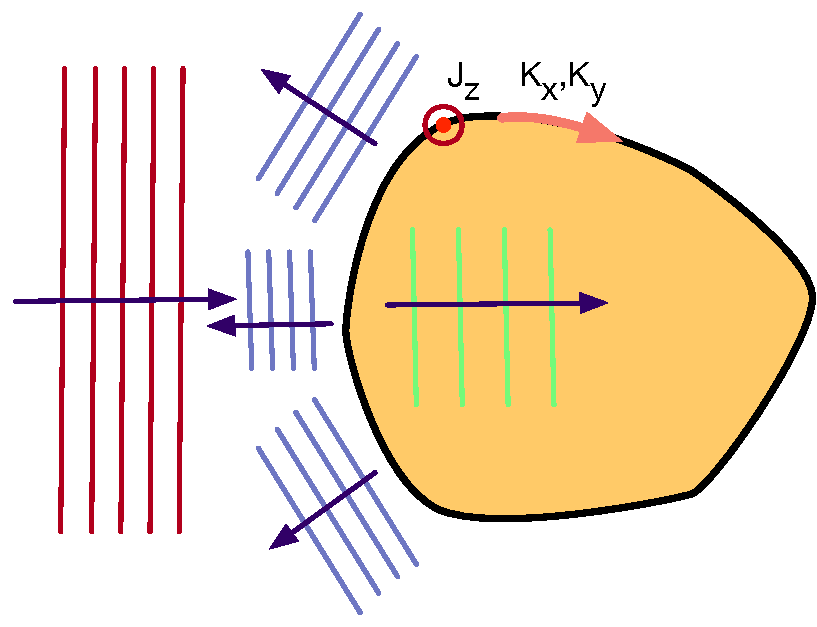
\includegraphics[width=1\columnwidth]{figures/Region}
\end{minipage}
\begin{minipage}{0.7\textwidth}
\begin{subequations}\label{Eq:IntegralEquations}
\begin{equation}
    E^s(r) = -i\omega\mu\iint_{S}G(r,r')[1+\frac{1}{k^2}\nabla'\nabla'\cdotp]J_s(r') \,dr' - \nabla \times \iint_{S}G(r,r')K_s(r') \,dr'
\end{equation}
\begin{equation}
    H^s(r) = -i\omega\epsilon\iint_{S}G(r,r')[1+\frac{1}{k^2}\nabla'\nabla'\cdotp]K_s(r') \,dr' + \nabla \times \iint_{S}G(r,r')J_s(r') \,dr'
\end{equation}
\end{subequations}
\end{minipage}

\begin{center}
The general 3D problem, showing an incident field on the volume $V_2$ producing a surface electric current density $J_s(r)$, which generates a scattered electric and magnetic field. For the 2D case (TEM) only $J_z$ and $K_x$, $K_y$ would be present. 
\end{center}

Because this is a scattering problem, the surface currents are not known. Therefore, the scattered fields have to be solved for in two steps:

\begin{enumerate}
\item $J_s$ and $K_s$ have to be solved using Eqs.\eqref{Eq:IntegralEquations} with the boundary conditions and the incident electromagnetic field
\item The scattered fields are evaluated by integrating the induced currents $J_s$ and $K_s$
\end{enumerate}

In most electromagnetic problems the only present surface current is the electric current $J_s$. This reduces the scattered field equations into:
\begin{align*}
    E^s(r) &= -i\omega\mu\iint_{S}G(r,r')[1+\frac{1}{k^2}\nabla'\nabla'\cdotp]J_s(r') \,dr'\\
    H^s(r) &= \nabla \times \iint_{S}G(r,r')J_s(r') \,dr'    
\end{align*}

These equations are commonly used by themselves to solve for the scattered electromagnetic fields, and are referred to as the Electric Field Integral Equation (EFIE) and the Magnetic Field Integral Equation (MFIE), respectively\cite{Method_Moments}.

\newpage
\section{Two Formulations for 2D and TEM solutions}

The above shows our initial formulation for the problem. In 2D we have:
\begin{enumerate}
    \item $n = [n_x,n_y,0]$
    \item $J = [0,0,J_z]$
    \item $K = [K_x,K_y,0]$
    \item $\frac{\partial}{\partial z} = 0$
\end{enumerate}
With Maxwell's equations being formulated as integral equations in the following way,

\begin{minipage}{0.45\textwidth}
\begin{align*}
\nabla \cdot E = 0 \quad \quad
& \nabla \cdot H = 0 \\
\nabla \times E = -\mu \frac{\partial H}{dt} + K\quad \quad 
& \nabla \times H = -\epsilon \frac{\partial E}{dt} + J
\end{align*}
\end{minipage}
$\longrightarrow$
\begin{minipage}{0.45\textwidth}
\begin{align*}
    E^s(\rho) &= -i\omega\mu(\mathcal{L}J_s)(\rho) - (\mathcal{R}K_s)(\rho)\\
    H^s(\rho) &= -i\omega\epsilon(\mathcal{L}K_s)(\rho) + (\mathcal{R}J_s)(\rho)
\end{align*}
\end{minipage}

\subsection{The Two Formulations}

There are, however two different formulations for the integral operators,

\begin{minipage}{0.45\textwidth}
\ \\
\begin{center} \bf Formulation as Implemented\end{center}
\begin{align*}
    (\mathcal{L}J)(\rho) &= \int_{\ell}G(\rho,\rho')[1+\frac{1}{k^2}\nabla'\nabla'\cdotp]J(\rho') \,d\rho'\\
    (\mathcal{R}J)(\rho) &= \int_{\ell} J(\rho') \times \nabla'  G(\rho,\rho')\,d\rho'\\
    (\mathcal{L}K)(\rho) &= \int_{\ell}G(\rho,\rho')[1+\frac{1}{k^2}\nabla'\nabla'\cdotp]K(\rho') \,d\rho'\\
    (\mathcal{R}K)(\rho) &= \int_{\ell} K(\rho') \times \nabla' G(\rho,\rho') \,d\rho'
\end{align*}
\end{minipage}
\begin{minipage}{0.45\textwidth}
\ \\
\begin{center} \bf  Alternative Formulation \end{center}
\begin{align*}
    (\mathcal{L}J)(\rho) &= \int_{\ell}[1+\frac{1}{k^2}\nabla\nabla\cdotp] [G(\rho,\rho')J(\rho')] \,d\rho'\\
    (\mathcal{R}J)(\rho) &= \int_{\ell}\nabla \times [G(\rho,\rho')J(\rho')] \,d\rho'\\
    (\mathcal{L}K)(\rho) &= \int_{\ell}[1+\frac{1}{k^2}\nabla\nabla\cdotp] [G(\rho,\rho')K(\rho')] \,d\rho'\\
    (\mathcal{R}K)(\rho) &= \int_{\ell}\nabla \times [G(\rho,\rho')K(\rho')] \,d\rho'
\end{align*}
\end{minipage}
\ \\

\subsection{The $\mathcal{R}X$ implementations are the same}

\begin{minipage}{0.45\textwidth}
\begin{align*}
    (\mathcal{R}X)(\rho) &= \int_{\ell} X(\rho') \times \nabla' G(\rho,\rho') \,d\rho'\\
    X \times \nabla' G = 
    &\begin{array}{|ccc|}
    \hat i & \hat j & \hat k\\
    X_x & X_y & X_z \\
    \frac{\partial G}{\partial x'} & \frac{\partial G}{\partial y'} & 0 \\
    \end{array}\\
    =  & - X_z \frac{\partial G}{\partial y'} \hat i + X_z \frac{\partial G}{\partial x'} \hat j + 
        \left(X_x \frac{\partial G}{\partial y'} - X_y \frac{\partial G}{\partial x'}\right) \hat k\\
    (\mathcal{R}X)(\rho) &=  
      \left[ \begin{array}{c} - X_z \frac{\partial G}{\partial y'}\\ X_z \frac{\partial G}{\partial x'} \\X_x \frac{\partial G}{\partial y'} - X_y \frac{\partial G}{\partial x'}   \end{array} \right]\\
        &= \left[ \begin{array}{ccc} 0 & 0 & - \frac{\partial G}{\partial y'}\\ 
                            0 & 0 &\frac{\partial G}{\partial x'}\\ 
                            \frac{\partial G}{\partial y'} &-\frac{\partial G}{\partial x'} &0 \end{array} \right]
        \left[ \begin{array}{c} 
        X_x \\ X_y \\ X_z \end{array} \right]
\end{align*}
\end{minipage}
\begin{minipage}{0.45\textwidth}
\begin{align*}
     (\mathcal{R}X)(\rho) &= \int_{\ell}\nabla \times [G(\rho,\rho')X(\rho')] \,d\rho'\\
      \nabla \times  (G X) &= 
    \begin{array}{|ccc|}
    \hat i & \hat j & \hat k\\
    \frac{\partial }{\partial x} & \frac{\partial }{\partial y} & 0 \\
    G X_x & G X_y & G X_z \\
    \end{array} \\ &\text{$X$ is not a function of $\rho = [x,y,z]$}
    \\
    &=  X_z \frac{\partial G}{\partial y} \hat i - X_z \frac{\partial G}{\partial x} \hat j + \left(X_y \frac{\partial G}{\partial x} - X_x \frac{\partial G}{\partial y}\right) \hat k\\
    (\mathcal{R}X)(\rho) &= 
      \left[ \begin{array}{c} X_z \frac{\partial G}{\partial y} \\ - X_z \frac{\partial G}{\partial x} \\X_y \frac{\partial G}{\partial x} - X_x \frac{\partial G}{\partial y}   \end{array} \right] \\
       &= \left[ \begin{array}{ccc} 0 & 0 & \frac{\partial G}{\partial y}\\ 
                            0 & 0 &-\frac{\partial G}{\partial x}\\ 
                            -\frac{\partial G}{\partial y} &\frac{\partial G}{\partial x} &0 \end{array} \right]
        \left[ \begin{array}{c} 
        X_x \\ X_y \\ X_z \end{array} \right]
\end{align*}
\end{minipage}\\

{\centering But $\nabla G = - \nabla' G$ so these are equivalent\ \\}

\subsection{The $\mathcal{L}X$ implementations have different implications}

\begin{minipage}{0.45\textwidth}
\ \\
\begin{center}  \bf Formulation as Implemented\end{center}
\begin{align*}
    (\mathcal{L}X)(\rho) &= \int_{\ell}G(\rho,\rho')[1+\frac{1}{k^2}\nabla'\nabla'\cdotp]X(\rho') \,d\rho'\\
\end{align*}
\end{minipage}
\begin{minipage}{0.45\textwidth}
\ \\
\begin{center}  \bf Alternative Formulation \end{center}
\begin{align*}
    (\mathcal{L}X)(\rho) &= \int_{\ell}[1+\frac{1}{k^2}\nabla\nabla\cdotp]G(\rho,\rho')]X(\rho') \,d\rho'\\
\end{align*}
\end{minipage}
\ \\
Let $\mathcal{L}X = \mathcal{L}_1 X + \mathcal{L}_2 X$ and both have in common:
\begin{align*}
    (\mathcal{L}_1 X)(\rho) &= \int_{\ell}G(\rho,\rho') X(\rho') \,d\rho' = 
    \left[ \begin{array}{c} G X_x\\ G X_y \\ G X_z  \end{array} \right] = \left[ \begin{array}{ccc} G & 0 & 0 \\ 
                            0 & G & 0\\ 
                            0 & 0 & G \end{array} \right]
        \left[ \begin{array}{c} 
        X_x \\ X_y \\ X_z \end{array} \right]
\end{align*}
which is easily evaluated (taking in account the singularity for $G$).
\ \\

\subsubsection{For $\mathcal{L}_2 X$ we have differentiated formulations}

\begin{minipage}{0.45\textwidth}
\ \\
\begin{center}  \bf Formulation as Implemented\end{center}
\begin{align*}
    (\mathcal{L}_2X)(\rho) &= \int_{\ell}G(\rho,\rho')\frac{1}{k^2}\nabla'\nabla'\cdotp X(\rho') \,d\rho'\\
    \nabla'\nabla'\cdotp X &= \nabla' (\frac{\partial X_x}{\partial x} + \frac{\partial X_y}{\partial y} + 0) 
    = \nabla' \left( \frac{\partial X_x}{\partial x} + \frac{\partial X_y}{\partial y} \right)\\
    &= \left( \frac{\partial^2 X_x}{\partial^2 x} + \frac{\partial^2 X_y}{\partial xy}\right) \hat i + 
    \left( \frac{\partial^2 X_x}{\partial yx} + \frac{\partial^2 X_y}{\partial^2 y}\right) \hat j + 
        0 \hat k\\
    (\mathcal{L}_2X)(\rho) &= \frac{1}{k^2}
    \left[ \begin{array}{c} G\left( \frac{\partial^2 X_x}{\partial^2 x} + \frac{\partial^2 X_y}{\partial xy}\right) \\ 
                            G\left( \frac{\partial^2 X_x}{\partial yx} + \frac{\partial^2 X_y}{\partial^2 y}\right)\\ 
                            0 
    \end{array} \right] \\ 
    &= \frac{G}{k^2} \left[ \begin{array}{ccc} \frac{\partial^2 }{\partial^2 x} & \frac{\partial^2 }{\partial xy}\ & 0 \\ 
                            \frac{\partial^2 }{\partial yx} & \frac{\partial^2 }{\partial^2 y} &0\\ 
                            0 & 0 &0 \end{array} \right]
        \left[ \begin{array}{c} 
        X_x \\ X_y \\ X_z \end{array} \right]
\end{align*}
\end{minipage}
\begin{minipage}{0.45\textwidth}
\ \\
\begin{center}  \bf Alternative Formulation \end{center}
\begin{align*}
    (\mathcal{L}_2 X)(\rho) &= \int_{\ell}\frac{1}{k^2}\nabla\nabla\cdotp [G(\rho,\rho')X(\rho')] \,d\rho'\\
       \nabla\nabla\cdotp &[G(\rho,\rho')X(\rho')] = \nabla \left(\frac{\partial (G X_x)}{\partial x} + \frac{\partial (G X_y)}{\partial y} + 0\right)\\
       &\text{$X$ is not a function of $\rho = [x,y,z]$}\\
    &= \left( X_x \frac{\partial^2 G}{\partial^2 x} + X_y \frac{\partial^2 G}{\partial xy}\right) \hat i + 
    \left( X_x \frac{\partial^2 G}{\partial yx} + X_y \frac{\partial^2 G}{\partial^2 y}\right) \hat j + 
        0 \hat k\\
    (\mathcal{L}_2X)(\rho) &= \frac{1}{k^2}
    \left[ \begin{array}{c} X_x \frac{\partial^2 G}{\partial^2 x} + X_y\frac{\partial^2 G}{\partial xy} \\ 
                            X_x \frac{\partial^2 G}{\partial yx} + X_y \frac{\partial^2 G}{\partial^2 y}\\ 
                            0 
    \end{array} \right] \\
    &= \frac{1}{k^2} \left[ \begin{array}{ccc} \frac{\partial^2 G }{\partial^2 x} & \frac{\partial^2 G }{\partial xy}\ & 0 \\ 
                            \frac{\partial^2 G}{\partial yx} & \frac{\partial^2 G}{\partial^2 y} &0\\ 
                            0 & 0 &0 \end{array} \right]
        \left[ \begin{array}{c} 
        X_x \\ X_y \\ X_z \end{array} \right]
\end{align*}
\end{minipage}
\ \\

In Gibson (2.4.3) it is shown that \cite{Method_Moments}:
\begin{align*}
    \nabla\nabla\cdotp [G(\rho,\rho')J(\rho')]  \equiv G(\rho,\rho')\nabla'\nabla'\cdotp J(\rho') 
\end{align*}
by the use of vector identities and some algebra.

The use of the ``Formulation as implemented'' seems to have issues; perhaps associated with the derivatives of $X$ which is a surface current. The other formulation simply requires the derivatives of the Green's function which would seem to be straightforward.

\newpage
\section{Green's Function and Derivatives}

We need a 2D Green's function and derivatives in order to evaluate the operators.

\subsection{Green's Function for 2D - Zero'th order 2nd Hankel function}
\begin{align*}
    G(x, y, x', y') = &-\frac{i}{4}H_0^{(2)}(k|\rho-\rho'|)\\
     &= -\frac{i}{4}H_0^{(2)}(k\sqrt{(x-x')^2+(y-y')^2})\\
     &= -\frac{i}{4}H_0^{(2)}(k r)\\
\end{align*}
\begin{align*}
     r &= ((x-x')^2+(y-y')^2)^{\frac{1}{2}} = |\rho-\rho'|\\
     \frac{\partial r}{\partial x} &= \frac{1}{2} ((x-x')^2+(y-y')^2)^{-\frac{1}{2}} 2 (x-x')\\ 
     & = \frac{(x-x')}{r} = \frac{(x-x')}{|\rho-\rho'|}\\
     \frac{\partial r}{\partial y}&=  \frac{(y-y')}{r} = \frac{(y-y')}{|\rho-\rho'|}\\
\end{align*}

\subsection{Derivatives of the Green's function}

\subsubsection{Derivatives of the Hankel function}

Derivative relationship,
\begin{align*}
    \left(\frac{1}{w}\frac{d}{dw}\right)^k (w^{-n} H_n^{(2)}(w)) &= (-1)^k w^{-n-k} H_{n+k}^{(2)}(w)\\
\end{align*}
Zero'th order for Green's function,
\begin{align*}
    \left(\frac{1}{w}\frac{d}{dw}\right)^k (w^{-0} H_0^{(2)}(w)) &= (-1)^k w^{-0-k} H_{0+k}^{(2)}(w)\\
    \left(\frac{1}{w}\frac{d}{dw}\right)^k H_0^{(2)}(w) &= (-1)^k w^{-k} H_{k}^{(2)}(w)
\end{align*}
First Derivative. $k = 1$:
\begin{align*}
    \left(\frac{1}{w}\frac{d}{dw}\right)^1 H_0^{(2)}(w) &= (-1)^1 w^{-1} H_{1}^{(2)}(w)\\
    \frac{1}{w}\frac{d}{dw} H_0^{(2)}(w) &= - \frac{1}{w} H_{1}^{(2)}(w)\\
    \frac{d}{dw} H_0^{(2)}(w) &= - H_{1}^{(2)}(w)
\end{align*}

We will also need derivative of $H_{1}^{(2)}$ so $k = 1$ $n = 1$
\begin{align*}
    \left(\frac{1}{w}\frac{d}{dw}\right)^k (w^{-n} H_n^{(2)}(w)) &= (-1)^k w^{-n-k} H_{n+k}^{(2)}(w)\\
    \left(\frac{1}{w}\frac{d}{dw}\right)^1 (w^{-1} H_1^{(2)}(w)) &= (-1)^1 w^{-1-1} H_{1+1}^{(2)}(w)\\
    \frac{1}{w}\frac{d}{dw} (\frac{1}{w} H_1^{(2)}(w)) &= - \frac{1}{w^{2}} H_{2}^{(2)}(w)\\
    \frac{d}{dw} (\frac{1}{w} H_1^{(2)}(w)) &= -\frac{1}{w} H_{2}^{(2)}(w)\\
    H_1^{(2)}(w) \frac{d}{dw} \left(\frac{1}{w}\right)  +  \frac{1}{w} \frac{d}{dw}  H_1^{(2)}(w) &= -\frac{1}{w} H_{2}^{(2)}(w)\\
    H_1^{(2)}(w) \left(\frac{-1}{w^2}\right)  +  \frac{1}{w} \frac{d}{dw}  H_1^{(2)}(w) &= -\frac{1}{w} H_{2}^{(2)}(w)\\
    \frac{1}{w} \frac{d}{dw}  H_1^{(2)}(w) &= -\frac{1}{w} H_{2}^{(2)}(w) -  \left(\frac{-H_1^{(2)}(w)}{w^2}\right)\\
    \frac{d}{dw}  H_1^{(2)}(w) &=  \frac{H_1^{(2)}(w)}{w} - H_{2}^{(2)}(w) \\
\end{align*}
However,
\begin{align*}
    \frac{n}{w} H_n^{(2)}(w) = \frac{H_{n-1}^{(2)}(w)}{2} + \frac{H_{n+1}^{(2)}(w)}{2}
    \longrightarrow \frac{H_1^{(2)}(w)}{w}  = \frac{H_{0}^{(2)}(w)}{2} + \frac{H_{2}^{(2)}(w)}{2} 
\end{align*}
So,
\begin{align*}
    \frac{d}{dw} H_0^{(2)}(w) = - H_{1}^{(2)}(w) \quad \text{and} \quad  
    \frac{d}{dw}  H_1^{(2)}(w) =   \frac{H_{0}^{(2)}(w)}{2} - \frac{H_{2}^{(2)}(w)}{2} \\
\end{align*}

\newpage
\subsection{Small argument versions of $H_0^2(|r|)$ function and derivatives}

We will need small argument forms of the $H_0^2(|r|)$ function and derivatives to the self-contribution of a surface element and nearby fields due to the presence of a singularity. 

\subsubsection{Small argument versions of $H_0^2(|r|)$}

Henkel function of interest is $H_0^2(|r|)$ for a small argument we have:
\begin{align*}
    H_0^{(2)}(w) = J_0(w) - i Y_0(w) 
\end{align*}
For small $w$,
\begin{align*}
    J_0(w) &= \frac{1}{\Gamma(1)} \left(\frac{w}{2}\right)^0 = 1\\
    Y_0(w) &= \frac{2}{\pi} \left(\ln \left( \frac{w}{2}\right) + \gamma\right) \quad \text{with} \quad \gamma = 0.5772\\
           &= \frac{2}{\pi} \left(\ln \left( \frac{w}{2}\right) + \ln e^\gamma_G \right) = \frac{2}{\pi} \left(\ln \left( e^\gamma_G \frac{w}{2}\right) \right) \\
           &= \frac{2}{\pi} \ln \left( \gamma_G \frac{w}{2} \right) \quad \gamma_G = 1.781 = e^\gamma\\
    H_0^{(2)}(w) &= 1 - i \frac{2}{\pi} \ln \left( \gamma_G \frac{w}{2} \right)
\end{align*}
and we have,
\begin{align*}
    H_0^2(|r|)_{sa} = 1 - i \frac{2}{\pi} \ln \left(\frac{\gamma_G}{2} |r| \right)
\end{align*}

\subsubsection{Small argument versions of $\frac{d}{dr}(H_0^2(|r|))$}

\begin{minipage}[t]{0.5\textwidth}
{\centering Direct Derivation\ \\}

\begin{align*}
    |r| &= \sqrt{r^2}\\
    x &= |r| \\
    \frac{dx}{dr} &= \frac{1}{2 \sqrt{r^2}} 2 r = \frac{r}{|r|}
\end{align*}
we also have,
\begin{align*}
    \frac{d}{dx}(H_0^2 (x)) = -H_1^2(x)
\end{align*}
and we have for the general derivative,
\begin{align*}
    \frac{dH_0^2}{dr} = \frac{d}{dx}(H_0^2 (x)) \frac{dx}{dr} = -H_1^2(|r|) \frac{r}{|r|}
\end{align*}

To get the small argument, 
\begin{align*}
    H_1^2(z) &= J_1(z) - i Y_1(z) \\
    \text{Small Argument:}& \\
    J_1(z) &= \frac{1}{\Gamma(2)} \frac{z}{2} = \frac{z}{2}\\
    Y_1(z) &= -\frac{2\Gamma(1)}{z\pi} + \frac{1}{\Gamma(2)} \frac{z}{2} \cot(\pi) \\
           &= -\frac{2}{\pi z} + \frac{z}{2} \cot(\pi)
\end{align*}
I think we drop the last term
\begin{align*}
     Y_1(z) &= -\frac{2}{\pi z}
\end{align*}
and we have,
\begin{align*}
     H_1^2(z)_{sa} &= \frac{z}{2} + i  \frac{2}{\pi z}
\end{align*}
and so,  
\begin{align*}
    \frac{d}{dr} \left( H_0^2(|r|) \right)_{sa} &= -\left(\frac{|r|}{2} + i \left(\frac{2}{\pi} \frac{1}{|r|} \right)\right) \frac{r}{|r|}\\
    &= -\left(\frac{r}{2} + i \frac{2}{\pi} \frac{1}{r} \right)
\end{align*}

\end{minipage}
\begin{minipage}[t]{0.5\textwidth}
{\centering Derivation From Small Argument $H_0^2(|r|)$\ \\}
\begin{align*}
    H_0^2(|r|)_{sa} &= 1 - i \frac{2}{\pi} \ln \left(\frac{\gamma}{2} |r| \right)\\
    w &= \frac{\gamma}{2} x \\
    \frac{dw}{dx} = \frac{\gamma}{2} \\
    x &= |r| \\
    \frac{dx}{dr} &= \frac{1}{2 \sqrt{r^2}} 2 r = \frac{r}{|r|}
    \frac{d}{dr} \ln(w) &= \frac{d}{dx}(\ln(x)) \frac{dx}{dr}  = \frac{1}{x} \frac{dx}{dr}\\
    x &= \frac{\gamma}{2} |r| \rightarrow \frac{dx}{dr} = \frac{\gamma}{2}\frac{r}{|r|}\\
\end{align*}
which gives,
\begin{align*}  
    \frac{d}{dr}\left(H_0^2 (|r|)_{sa}\right) & = - i \frac{2}{\pi} \frac{d}{dw} (\ln w) \frac{dw}{dx} \frac{dx}{dr} 
    = - i \frac{2}{\pi} \frac{1}{w} \frac{\gamma}{2} \frac{r}{|r|} \\
    &= - i \frac{2}{\pi} \frac{2}{\gamma_G |r|} \frac{\gamma}{2} \frac{r}{|r|} \\
    &= - i \frac{2}{\pi} \frac{1}{|r|}\frac{r}{|r|}  = - i \frac{2}{\pi} \frac{1}{r} \\
\end{align*}
\end{minipage}

\subsubsection{Small argument versions of $\frac{d^2}{dr^2}(H_0^2(|r|))$}

\begin{minipage}[t]{0.5\textwidth}
{\centering Direct Derivation\ \\}

We have for the general derivative,
\begin{align*}
    \frac{d}{dr} \left(H_0^2(|r|)\right) &= -H_1^2(|r|) \frac{r}{|r|}\\
    \frac{d^2}{dr^2} \left(H_0^2(|r|)\right) &= -\left(\frac{H_0^2(|r|) - H_2^2 (|r|)}{2} \right) \frac{r}{|r|} \frac{r}{|r|}\\
                               &=-\frac{1}{2}\left(H_0^2(|r|) - H_2^2(|r|) \right)
\end{align*}
To get the small argument, 
\begin{align*}
\text{Small Argument:}&\\
    H_0^2(|r|) & = 1 - i \frac{2}{\pi} \ln \left( \frac{\gamma_G |r|}{2} \right)\\
    H_2^2(z) &= J_2(z) - i Y_2(z) \\
    \text{Small Argument:}& \\
    J_2(z) &= \frac{1}{\Gamma(3)} (\frac{z}{2})^2 = \frac{z^2}{8}\\
    Y_2(z) &= -\frac{2\Gamma(2)}{\pi} \left(\frac{2}{z}\right)^2 + \frac{1}{\Gamma(3)} \left(\frac{z}{2}\right)^2 \cot(2\pi) \\
           &= -\frac{4}{\pi z^2} + \frac{z^2}{4} \cot(2\pi)
\end{align*}
Again I think we drop the last term,
\begin{align*}
    H_2^2(z)_{sa} &=  \frac{z^2}{8} + i \left( \frac{4}{\pi z^2} \right) 
\end{align*}
which gives,
\begin{align*}
    \frac{d^2}{dr^2} \left( H_0^2(|r|) \right)_{sa} &= -\frac{1}{2} \left( 1 - i \frac{2}{\pi} \ln \left( \frac{\gamma_G |r|}{2} \right) - \left( \frac{|r|^2}{8} + i \left( \frac{4}{\pi |r|^2} \right) \right) \right)
\end{align*}
\end{minipage}
\begin{minipage}[t]{0.5\textwidth}
{\centering Derivation From Small Argument $H_0^2(|r|)_{sa}$\ \\}

\begin{align*}
\frac{d}{dr}\left(H_0^2(|r|)_{sa}\right) & =  - i \frac{2}{\pi} \frac{1}{r} \\
\frac{d^2}{dr^2}\left(H_0^2 (|r|)_{sa}\right) & =  i \frac{2}{\pi} \frac{1}{r^2} \\
\end{align*}

\end{minipage}


\begin{minipage}{0.7\textwidth}
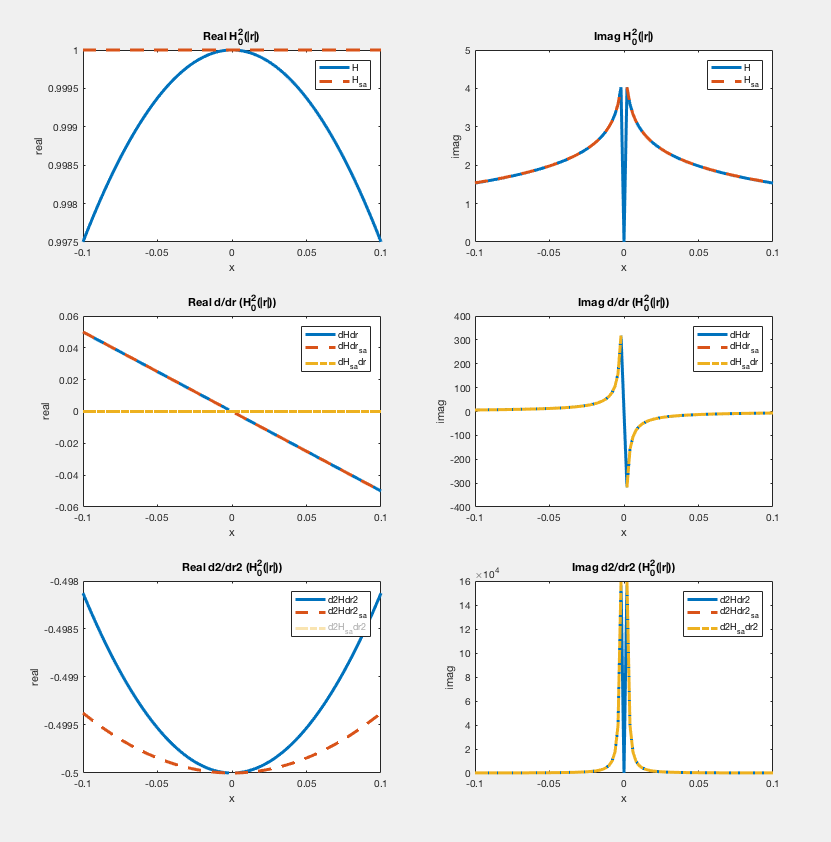
\includegraphics[width=1\columnwidth]{figures/OneDGreensFct}
\end{minipage}
\begin{minipage}{0.3\textwidth}
    {\centering Comparison of Small Argument values\ \\}
    \begin{enumerate}
        \item Real part of small argument $H_0^2(|r|)$ is constant not slightly varying. 
        \item Therefore derivatives for real part of $\frac{d}{dr}\left(H_0^2|_{sa} (|r|)\right)$ and $\frac{d^2}{dr^2}\left(H_0^2|_{sa} (|r|)\right)$ are zero.
        \item Slight error in real part for direct determination of $\frac{d^2}{dr^2}\left(H_0^2|_{sa} (|r|)\right)$.
    \end{enumerate}
\end{minipage}


\subsection{Derivatives of the Green's function}
For our case we have $w = kr$ we have,
\begin{align*}
    \frac{d}{dx} H_0^{(2)}(w) &=  \frac{d}{dw} H_0^{(2)}(w) \frac{dw}{dr} \frac{dr}{dx} = - H_{1}^{(2)}(w) k  \frac{(x-x')}{r} \\  
    \frac{d}{dy} H_0^{(2)}(w) &=  \frac{d}{dw} H_0^{(2)}(w) \frac{dw}{dr} \frac{dr}{dy} = - H_{1}^{(2)}(w) k  \frac{(y-y')}{r} \\  
    \frac{d}{dx}  H_1^{(2)}(w) &= \frac{d}{dw}  H_1^{(2)}(w) \frac{dw}{dr} \frac{dr}{dx}  = \left(\frac{H_{0}^{(2)}(w)}{2} - \frac{H_{2}^{(2)}(w)}{2} \right)  k  \frac{(x-x')}{r}\\
    \frac{d}{dy}  H_1^{(2)}(w) &= \frac{d}{dw}  H_1^{(2)}(w) \frac{dw}{dr} \frac{dr}{dy}  = \left(\frac{H_{0}^{(2)}(w)}{2} - \frac{H_{2}^{(2)}(w)}{2} \right)  k  \frac{(y-y')}{r}\\
\end{align*}


Now derivatives of Green's function,
\begin{align*}
    \frac{\partial G}{\partial x} &= \frac{\partial }{\partial x} \left[ -\frac{i}{4}H_0^{(2)}(w) \right] = -\frac{i}{4} \frac{\partial H_0^{(2)}(w)}{\partial x} \\
    &= \frac{ik}{4}  H_{1}^{(2)}(kr) \frac{(x-x')}{r}
\end{align*}
likewise, 
\begin{align*}
    \frac{\partial G}{\partial y} &= \frac{ik}{4}  H_{1}^{(2)}(kr) \frac{(y-y')}{r}
\end{align*}
Which comports with Scott's equations (sign change due to derivatives wrt to $x'$ or $y'$),
\begin{align*}
    \frac{\partial G}{\partial y'} = -\frac{i}{4}\frac{k(y-y')H_1^{(2)}(k|\rho-\rho'|)}{|\rho-\rho'|} \quad &,\quad
    \frac{\partial G}{\partial x'} = -\frac{i}{4}\frac{k(x-x')H_1^{(2)}(k|\rho-\rho'|)}{|\rho-\rho'|}
\end{align*}

For the 2nd formulation we also need higher order derivatives,
\begin{align*}
    \frac{\partial^2 G}{\partial^2 x} &= \frac{ik}{4} \frac{\partial }{\partial x} \left[H_{1}^{(2)}(kr) \frac{(x-x')}{r} \right]\\
    &= \frac{ik}{4} \left[ \frac{(x-x')}{r} \frac{\partial }{\partial x} H_{1}^{(2)}(kr)  + 
                        H_{1}^{(2)}(kr) \frac{\partial }{\partial x}  \frac{(x-x')}{r} \right] \\
    &= \frac{ik}{4} \left[ \frac{(x-x')}{r} \left( \frac{H_{0}^{(2)}(kr)}{2} - \frac{H_{2}^{(2)}(kr)}{2} \right) k \frac{(x-x')}{r}  + 
                        H_{1}^{(2)}(kr) \left( \frac{1}{r} - (x-x')\frac{1}{r^2} \frac{\partial r} {\partial x} \right) \right] \\
    &= \frac{ik}{4} \left[ k \frac{(x-x')^2}{r^2} \left( \frac{H_{0}^{(2)}(kr)}{2} - \frac{H_{2}^{(2)}(kr)}{2} \right)  + H_{1}^{(2)}(kr) \left( \frac{1}{r} - \frac{1}{r^2} \frac{(x-x')^2}{r} \right) \right] \\
    &= \frac{ik}{4} \left[ \frac{k(x-x')^2}{r^2} \left( \frac{H_{0}^{(2)}(kr)}{2} - \frac{H_{2}^{(2)}(kr)}{2} \right) + 
        H_{1}^{(2)}(kr)\left(\frac{1}{r} - \frac{(x-x')^2}{r^3} \right)  \right] \\
\end{align*}

\begin{align*}
    \frac{\partial^2 G}{\partial yx} &= \frac{ik}{4} \frac{\partial }{\partial y} \left[H_{1}^{(2)}(kr) \frac{(x-x')}{r} \right]\\
    &= \frac{ik}{4} \left[ \frac{(x-x')}{r} \frac{\partial }{\partial y} H_{1}^{(2)}(kr)  + 
                        H_{1}^{(2)}(kr) \frac{\partial }{\partial y}  \frac{(x-x')}{r} \right] \\
    &= \frac{ik}{4} \left[ \frac{(x-x')}{r} \left( \frac{H_{0}^{(2)}(kr)}{2} - \frac{H_{2}^{(2)}(kr)}{2} \right) k \frac{(y-y')}{r}  + 
                        H_{1}^{(2)}(kr) \left( \frac{0}{r} - (x-x')\frac{1}{r^2} \frac{\partial r} {\partial y} \right) \right] \\
    &= \frac{ik}{4} \left[ k \frac{(x-x')(y-y')}{r^2} \left( \frac{H_{0}^{(2)}(kr)}{2} - \frac{H_{2}^{(2)}(kr)}{2} \right)  - H_{1}^{(2)}(kr) \frac{1}{r^2} \frac{(x-x')(y-y')}{r}  \right] \\
    &= \frac{ik}{4} \left[ \frac{k(x-x')(y-y')}{r^2} \left( \frac{H_{0}^{(2)}(kr)}{2} - \frac{H_{2}^{(2)}(kr)}{2} \right) -
        H_{1}^{(2)}(kr)\frac{(x-x')(y-y')}{r^3}  \right] \\
\end{align*}

\begin{align*}
    \frac{\partial^2 G}{\partial^2 y} &= \frac{ik}{4} \frac{\partial }{\partial y} \left[H_{1}^{(2)}(kr) \frac{(y-y')}{r} \right]\\
    &= \frac{ik}{4} \left[ \frac{(y-y')}{r} \frac{\partial }{\partial y} H_{1}^{(2)}(kr)  + 
                        H_{1}^{(2)}(kr) \frac{\partial }{\partial y}  \frac{(y-y')}{r} \right] \\
    &= \frac{ik}{4} \left[ \frac{(y-y')}{r} \left( \frac{H_{0}^{(2)}(kr)}{2} - \frac{H_{2}^{(2)}(kr)}{2} \right) k \frac{(y-y')}{r}  + 
                        H_{1}^{(2)}(kr) \left( \frac{1}{r} - (y-y')\frac{1}{r^2} \frac{\partial r} {\partial y} \right) \right] \\
    &= \frac{ik}{4} \left[ k \frac{(y-y')^2}{r^2} \left( \frac{H_{0}^{(2)}(kr)}{2} - \frac{H_{2}^{(2)}(kr)}{2} \right)  + H_{1}^{(2)}(kr) \left( \frac{1}{r} - \frac{1}{r^2} \frac{(y-y')^2}{r} \right) \right] \\
    &= \frac{ik}{4} \left[ \frac{k(y-y')^2}{r^2} \left( \frac{H_{0}^{(2)}(kr)}{2} - \frac{H_{2}^{(2)}(kr)}{2} \right) + 
        H_{1}^{(2)}(kr)\left(\frac{1}{r} - \frac{(y-y')^2}{r^3} \right)  \right] \\
\end{align*}

\begin{align*}
    \frac{\partial^2 G}{\partial xy} &= \frac{ik}{4} \frac{\partial }{\partial x} \left[H_{1}^{(2)}(kr) \frac{(y-y')}{r} \right]\\
    &= \frac{ik}{4} \left[ \frac{(y-y')}{r} \frac{\partial }{\partial x} H_{1}^{(2)}(kr)  + 
                        H_{1}^{(2)}(kr) \frac{\partial }{\partial x}  \frac{(y-y')}{r} \right] \\
    &= \frac{ik}{4} \left[ \frac{(y-y')}{r} \left( \frac{H_{0}^{(2)}(kr)}{2} - \frac{H_{2}^{(2)}(kr)}{2} \right) k \frac{(x-x')}{r}  + 
                        H_{1}^{(2)}(kr) \left( \frac{0}{r} - (y-y')\frac{1}{r^2} \frac{\partial r} {\partial x} \right) \right] \\
    &= \frac{ik}{4} \left[ k \frac{(y-y')(x-x')}{r^2} \left( \frac{H_{0}^{(2)}(kr)}{2} - \frac{H_{2}^{(2)}(kr)}{2} \right)  - H_{1}^{(2)}(kr) \frac{1}{r^2} \frac{(y-y')(x-x')}{r}  \right] \\
    &= \frac{ik}{4} \left[ \frac{k(x-x')(y-y')}{r^2} \left( \frac{H_{0}^{(2)}(kr)}{2} - \frac{H_{2}^{(2)}(kr)}{2} \right) -
        H_{1}^{(2)}(kr)\frac{(x-x')(y-y')}{r^3}  \right] \\
\end{align*}

\begin{minipage}{0.75\textwidth}
{\centering

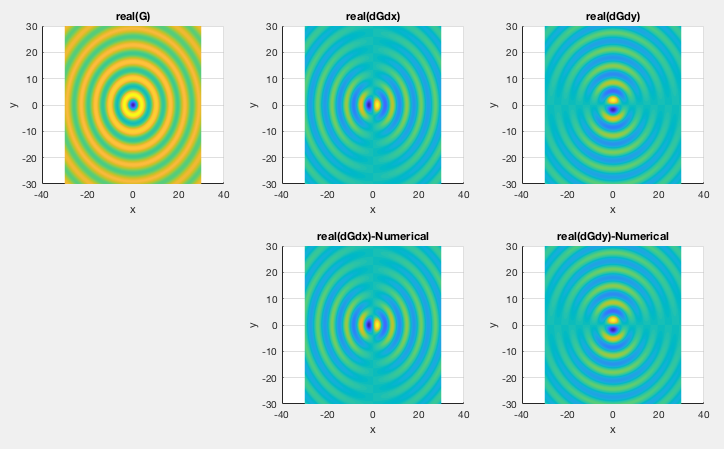
\includegraphics[width=0.75\columnwidth]{figures/GFirstDs}

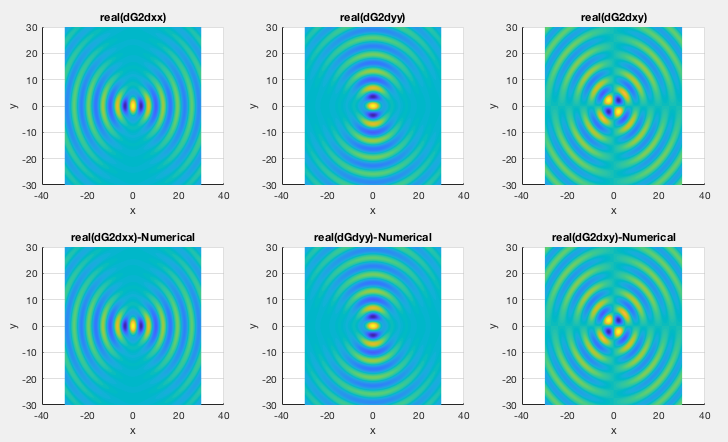
\includegraphics[width=0.75\columnwidth]{figures/G2ndDs}

}
\end{minipage}
\begin{minipage}{0.25\textwidth}
\begin{enumerate}
    \item $G$ is symmetrical in both $x$ and $y$.
    \item $\partial G/ \partial x$ is anti-symmetrical in  $x$ and symmetrical in $y$.
    \item $\partial G/ \partial y$ is symmetrical in $x$ and anti-symmetrical in $y$.
    \item $\partial^2 G/ \partial x^2$ and $\partial^2 G/ \partial x^2$ is symmetrical in both
    \item $\partial^2 G/ \partial xy$ and $\partial^2 G/ \partial yx$ is anti-symmetrical in both
\end{enumerate}
\end{minipage}

\newpage
\subsection{Singularities of the Green's Function and its derivatives}

When forming the scattered field equation to solve for $J_s$ and $K_s$ by evaluating the contour integral equations one of the segments will lie on $\rho' = \rho$, which represents a singularity of the Green's function and the derivatives.  
\ \\

Because the line segment ($\delta \ell$) is very small, we can assume that the field $X(\rho')$ is constant along the length. This simplifies the equation to an integration of the operator over the segment. Because the integral is being evaluated very close to the Green's function singularity we need to use the small-argument approximation of the Green's function \cite{Method_Moments}. The small-argument approximation of the Henkel function is:
\begin{align*}
    H_0^{(2)}(|\rho-\rho'|)_{sa} &= 1 - i \frac{2}{\pi} \ln \left( \gamma_G \frac{|\rho-\rho'|}{2} \right)
\end{align*}
and we have,
\begin{align*}
\label{Eq:SegmentIntegration}
    G(\rho, \rho') &= -\frac{i}{4}H_0^{(2)}(k|\rho-\rho'|) \\
    G(\rho, \rho')_{sa} &= -\frac{i}{4} \left( 1 - \frac{2i}{\pi} \ln \left( \gamma_G \frac{kr}{2}\right) \right)\\
\end{align*}
with $r = \sqrt{(x-x')^2+(y-y')^2}$. Using this small argument approximation we need to evaluate:
\begin{align*}
    \int_{\delta\ell} G(\rho,\rho')\, d\rho', \quad
    \int_{\delta\ell}\frac{\partial}{\partial x}G(\rho,\rho')\, d\rho', \quad
    \int_{\delta\ell}\frac{\partial}{\partial y}G(\rho,\rho')\, d\rho', \quad
    \int_{\delta\ell}\frac{\partial^2}{\partial x^2}G(\rho,\rho')\, d\rho', \quad
    \int_{\delta\ell}\frac{\partial^2}{\partial y^2}G(\rho,\rho')\, d\rho', \quad
    \int_{\delta\ell}\frac{\partial^2}{\partial y^2}G(\rho,\rho')\, d\rho'
\end{align*}

\subsubsection{Solving the Singularity of $G(\rho, \rho')$}
\begin{align*}
    \int_{-\delta\ell/2}^{\delta\ell/2} G(\rho,\rho')\, d\rho' &= -\frac{i}{4} \int_{-\delta\ell/2}^{\delta\ell/2}  \left( 1 - \frac{2i}{\pi} \ln \left( \gamma_G \frac{kr}{2}\right) \right) d\rho' \\
        &= -\frac{i}{4} \left( \int_{-\delta\ell/2}^{\delta\ell/2}  d\rho' - \int_{-\delta\ell/2}^{\delta\ell/2} \frac{2i}{\pi} \ln \left( \gamma_G \frac{k |\rho - \rho'|}{2}\right)d\rho' \right)  \\
     % \rho \rightarrow 0 \\
     \int_{-\delta\ell/2}^{\delta\ell/2} G(\rho,\rho')\, d\rho' &= -\frac{i}{4} \left( \delta \ell - \frac{2i}{\pi} \int_{-\delta\ell/2}^{\delta\ell/2} \ln \left( \gamma_G \frac{k |\rho - \rho'|}{2}\right)d\rho' \right)  \\
     &= -\frac{i}{4} \left( \delta \ell - \frac{2i}{\pi} \int_{-\delta\ell/2}^{\delta\ell/2} \ln \left|\gamma_G \frac{k (\rho - \rho')}{2}\right |d\rho' \right) 
\end{align*}
Let, 
\begin{align*}
    w = \frac{\gamma_G k}{2}(\rho-\rho')&, \quad dw  = -\frac{\gamma_G k}{2} d\rho'\\ 
    \rho'|_l = - \delta \ell/2 \rightarrow w_l = \frac{\gamma_G k (2\rho+\delta \ell)}{4}&, \quad \rho'|_u =  \delta \ell/2 \rightarrow w_u = \frac{\gamma_G k (2\rho-\delta \ell)}{4}
\end{align*}
gives 
\begin{align*}
     \int_{-\delta\ell/2}^{\delta\ell/2} G(\rho,\rho')\, d\rho' &= -\frac{i}{4} \left( \delta \ell + 
     \frac{2i}{\pi} \int_{w_l}^{w_u} \ln | w | \frac{-2}{\gamma_G k} dw \right)\\
     &= -\frac{i}{4} \left( \delta \ell - \frac{2i}{\pi} \frac{2}{\gamma_G k} \int_{w_l}^{w_u} \ln | w |  dw  \right)
\end{align*}

This has a weak singularity and needs to be solved in a Cauchy Principle Value sense, 
\begin{align*}
     \int_{-\delta\ell/2}^{\delta\ell/2} G(\rho,\rho')\, d\rho' 
     &= -\frac{i}{4} \left( \delta \ell -  \frac{2i}{\pi} \frac{2}{\gamma_G k} \lim_{\epsilon \to 0} \left[ \int_{w_l}^{\epsilon} \ln | w |  dw +  \int_{\epsilon}^{w_u} \ln | w |  dw\right] \ \right)\\
     &= -\frac{i}{4} \left( \delta \ell - \lim_{\epsilon \to 0} \left[\frac{2i}{\pi} \frac{2}{\gamma_G k} \int_{w_l}^{\epsilon} \ln | w |  dw + \frac{2i}{\pi} \frac{2}{\gamma_G k} \int_{\epsilon}^{w_u} \ln | w |  dw\right] \ \right)\\
\end{align*}

Integral of $\int \ln |w| dw  = w \ln |w| - w + C$
\begin{align*}
     \int_{-\delta\ell/2}^{\delta\ell/2} G(\rho,\rho')\, d\rho' 
     &= -\frac{i}{4} \left( \delta \ell - \frac{2i}{\pi} \frac{2}{\gamma_G k} \lim_{\epsilon \to 0} \left[ \left[w \ln | w | - w + C \right]_{w_l}^{\epsilon} + \left[ w \ln | w | - w + C \right]_{\epsilon}^{w_u} \right] \right)\\
      &= -\frac{i}{4} \left( \delta \ell - \frac{2i}{\pi} \frac{2}{\gamma_G k} \lim_{\epsilon \to 0} \left[ \epsilon \ln | \epsilon | - \epsilon + C - (w_l \ln | w_l | - w_l + C)  + (w_u \ln | w_u | - w_u + C  - ( \epsilon \ln | \epsilon | - \epsilon + C)  \right] \right)\\
    &= -\frac{i}{4} \left( \delta \ell - \frac{2i}{\pi} \frac{2}{\gamma_G k} \left[ w_u \ln | w_u |  - w_l \ln | w_l | - w_u + w_l) \right] \right) \\
\end{align*}
For the self-element singularity we have $\rho = \rho' = 0$, $w_l = \frac{\gamma_G k \delta \ell}{4}$ and $w_u = -\frac{\gamma_G k (\delta \ell)}{4}$
\begin{align*}
     \int_{-\delta\ell/2}^{\delta\ell/2} G(\rho,\rho')\, d\rho' 
    &= -\frac{i}{4} \left( \delta \ell - \frac{2i}{\pi} \frac{2}{\gamma_G k} \left[ \frac{\gamma_G k \delta \ell}{4} \ln | \frac{\gamma_G k \delta \ell}{4} |  - \frac{-\gamma_G k \delta \ell}{4} \ln | \frac{-\gamma_G k \delta \ell}{4} | - \frac{\gamma_G k \delta \ell}{4} + \frac{-\gamma_G k \delta \ell}{4}) \right] \right)\\
    &= -\frac{i}{4} \left( \delta \ell - i \frac{\delta \ell}{\pi} \left[  2 \ln | \frac{\gamma_G k \delta \ell}{4} |  - 2  \right] \right)\\
    &= -\frac{i}{4} \left(1 - i \frac{2 }{\pi} \ln | \frac{\gamma_G k \delta \ell}{4} |  + i \frac{2}{\pi} \right) \delta \ell
\end{align*}
Which is what Scott used,
\begin{align*}
    \int_{\delta\ell} G(\rho,\rho')\, d\rho' = -\frac{i}{4} \left( 1 + i \frac{2}{\pi} -  i \frac{2}{\pi} \ln \left(\frac{\gamma_G k \delta \ell}{4}\right) \right) \delta \ell;
\end{align*}
except for using $\gamma$ not $\gamma_G$.

Gibson appears to give this as (Eq. 5.15) as,
\begin{align*}
    \int_0^{\delta\ell} G(\rho,\rho')\, d\rho' &=  - \frac{i}{4} \delta \ell \left[1 - i \frac{2}{\pi} \ln \left(\frac{\gamma_G k \delta \ell}{4e} \right) \right] \\
    &=  -\frac{i}{4} \left[1 - i \frac{2}{\pi} \ln \left(\frac{\gamma_G k \delta \ell}{4e} \right) \right] \delta \ell\\ 
    &=  -\frac{i}{4} \left[1 - i \frac{2}{\pi} \left( \ln \left(\frac{\gamma_G k \delta \ell}{4}\right) - \ln(e) \right) \right] \delta \ell\\ 
    &=  -\frac{i}{4} \left[1 - i \frac{2}{\pi} \ln \left(\frac{\gamma_G k \delta \ell}{4}\right) + i \frac{2}{\pi} \right] \delta \ell\\ 
\end{align*}
which is integrated over different limits $ 0 \rightarrow \delta \ell$ but gives the same result.

\begin{minipage}{0.5\textwidth}
{\centering
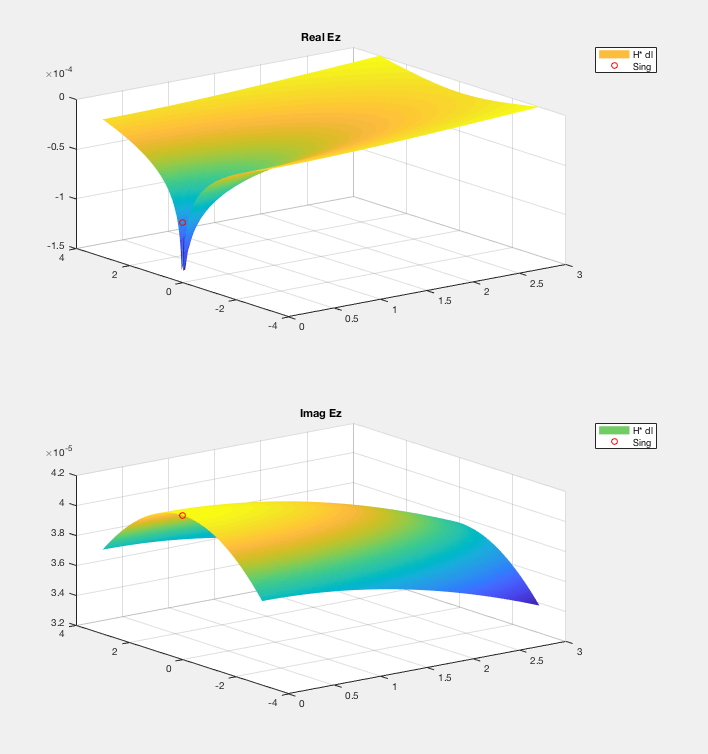
\includegraphics[width=0.95\columnwidth]{figures/GSingSurf2.png}
}
\end{minipage}
\begin{minipage}{0.5\textwidth}
\begin{enumerate}
    \item Surface is $\int_{\delta \ell} G d\rho' \approx G \delta \ell$ which is $-\infty$ at $\rho = \rho'$.
    \item Marker is singular value. 
    \item axis are in units of dl
    \item Symmetrical in x and y
\end{enumerate}
\end{minipage}

\begin{minipage}{0.5\textwidth}
{\centering
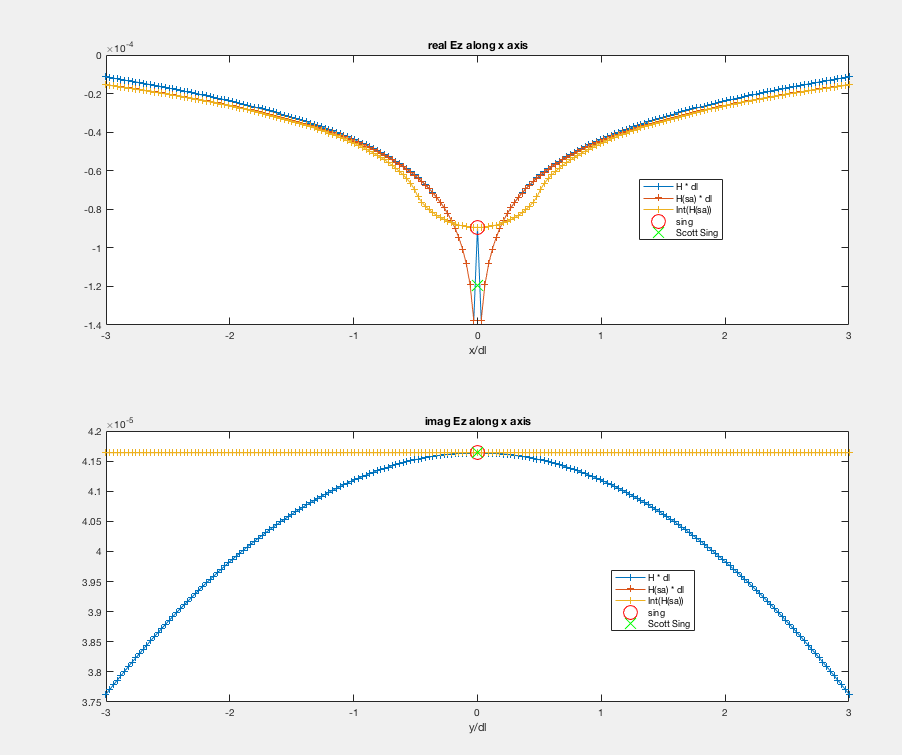
\includegraphics[width=0.95\columnwidth]{figures/GSing}
}
\end{minipage}
\begin{minipage}{0.5\textwidth}
\begin{enumerate}
    \item Plot $\int_{\delta \ell} G d\rho'$ along $x$ axis.
    \item Blue is $\int_{\delta \ell} G d\rho' = G \delta \ell$ except at singularity
    \item Red is smal arg approx $\int_{\delta \ell} G d\rho' = G \delta \ell$
    \item Yellow is $\int_{\delta \ell} G d\rho'$ for explicit integration of small arg G. 
    \item Red marker is singularity
    \item Green marker is Scott's value for singularity.
\end{enumerate}
\end{minipage}
\ \\
{\bf Conclusions:}
\begin{enumerate}
    \item Should use $\gamma_G$
    \item $\delta \ell$ should be small enough that small argument approx is good. For our case $|kr| < 1 \rightarrow |r| < 1/k = \lambda_0/2\pi$ 
    \item Need to use explicit integration for points that include the singularity i.e. $|\rho-\rho'| \le \delta \ell$. This explains some plotting artifacts.
\end{enumerate}

\begin{minipage}{0.5\textwidth}
{\centering
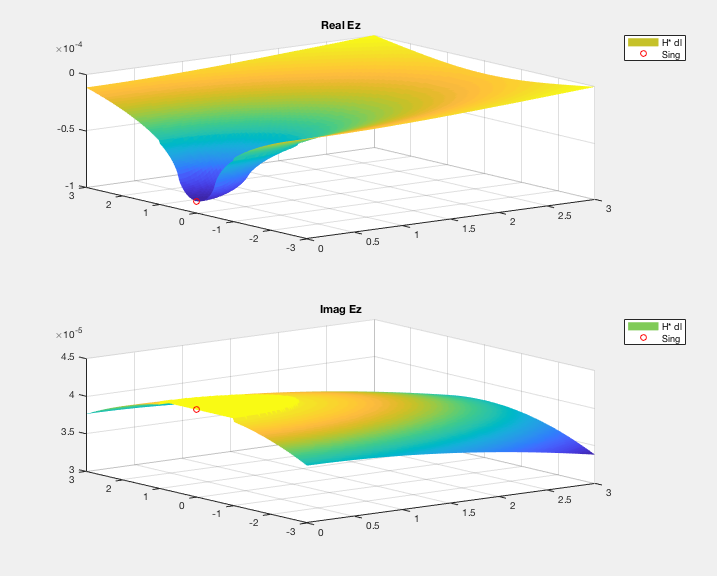
\includegraphics[width=0.95\columnwidth]{figures/GSingMod}\\
$\int_{\delta \ell} G dl$ using $G \delta \ell$ or explicit integration near singularity
}
\end{minipage}
\begin{minipage}{0.5\textwidth}
Code for using small argument integration near singularity,

\begin{minted}{matlab}

function [IG] = IGf(R,dl,k)
global c_gamma
IG = -1i/4*besselh(0,2,k*R)*dl;
IG(isnan(IG)) = -1i/4*(1 + 1i*2/pi - ...
    1i*2/pi*log(c_gamma*k*dl/4))*dl;
end

function [IG] = IGfSAI(R,dl,k)
global c_gamma
% w = c_gamma*k/2*(R-0);
wl = c_gamma*k/4*(2*R-dl);
wu = c_gamma*k/4*(2*R+dl);
IG = -1i/4.*(dl - 2i/pi.*2/c_gamma/k.*(wu.*log(abs(wu)) ...
     - wl.*log(abs(wl)) - wu + wl));
end

function [IG] = IGfm(R,dl,k)
sz = size(R);
S = reshape(R,sz(1)*sz(2),1);
IG(S > dl) = IGf(S(S > dl),dl,k);
IG(S <= dl) = IGfSAI(S(S<= dl),dl,k);
IG = reshape(IG,sz);
% end
\end{minted}

\end{minipage}

\subsubsection{Solving the Singularities of $\frac{\partial}{\partial x} G(\rho, \rho')$ and $\frac{\partial}{\partial y} G(\rho, \rho')$}

{\ \\ \centering \bf Change of variables\ \\ \ \\}

For dealing with these cases it will be useful to define a new coordinate systems $[u,v]$ and $[u',v']$ using the following,\\ \

\begin{minipage}{0.3\textwidth}
\begin{center}
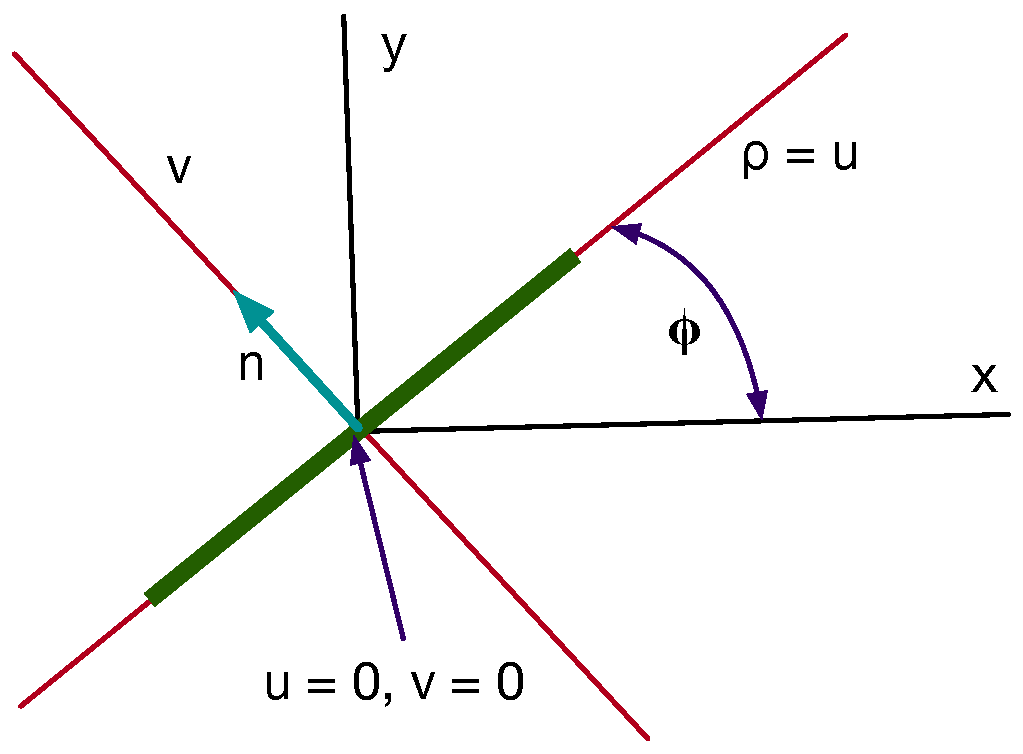
\includegraphics[width=1\columnwidth]{figures/Seg}\ \\
Rotation of the coordinate system for integration
\end{center}
\end{minipage}
\begin{minipage}{0.7\textwidth}
Because the variable $\rho'$ is not along a singular variable a change of variables is performed. The goal is to make it so that the integrand is a simple function of the variable that is being integrated over. The current variables are changed:
\begin{align*}
    \rho &= u \quad  \rho' = u'\\
    x &= u\cos(\theta) - v\sin(\theta)\\
    y &= u\sin(\theta) + v\cos(\theta)\\
    x' &= u'\cos(\theta) - v'\sin(\theta)\\
    y' &= u'\sin(\theta) + v'\cos(\theta)\\
    \sin(\theta) &= - n \cdot \hat x \quad \cos(\theta) = n \cdot y
\end{align*}
\noindent where $u$ and $v$ is the new coordinate system such that the line segment lies on the $v = 0$ line and $\hat{n}$ is in the direction of $\hat{v}$. Our point $\rho$ will be chosen so that it is an infinitesimal amount above the surface at $\rho = (u,v)$. 
\end{minipage}

\  \\
\pagebreak
{\ \\ \centering \bf Starting from the small argument form $H_0^2(|r|)_{sa}$\ \\\ \\}

\noindent{\bf First $\partial G/\partial x$:}
Differentiating the small argument Green's function with respect to $x$ yields us:
\begin{align*}
    \frac{\partial}{\partial x} G(\rho, \rho')_{sa} &= \frac{\partial}{\partial x} \left[ -\frac{i}{4} - \frac{1}{2\pi}\ln\left(\frac{\gamma_G k}{2} r \right) \right]\\
    &= - \frac{1}{2\pi}\frac{\partial}{\partial x} \left[\ln\left(\frac{\gamma_G k}{2} r \right) \right] = - \frac{1}{2\pi}\frac{1}{\frac{\gamma_G k}{2} r} \frac{\gamma_G k}{2} \frac{\partial r}{\partial x} = - \frac{1}{2\pi}\frac{1}{r}  \frac{(x-x')}{r} \\
    &=-\frac{1}{2\pi} \frac{(x-x')}{(x-x')^2+(y-y')^2}
\end{align*}
Integrating from $-\delta \ell/2$ to $\delta \ell/2$ yields us the following integral:
\begin{equation}\label{Eq:PreChangeOfVariablesIntegralX}
    \int_{\delta\ell}\frac{\partial}{\partial x}G(\rho,\rho')\, d\rho' = - \int_{-\frac{\delta \ell}{2}}^{\frac{\Delta l}{2}} \frac{1}{2\pi} \frac{(x-x')}{(x-x')^2+(y-y')^2}\, d\rho'
\end{equation}
\ \\

Applying this change of variables to Eq.~\eqref{Eq:PreChangeOfVariablesIntegral} yields:
\begin{align*}
    \int_{\delta\ell}\frac{\partial}{\partial x}G(\rho,\rho')\, d\rho' &= -\frac{1}{2\pi}\int_{-\frac{\delta \ell}{2}}^{\frac{\delta \ell}{2}}\frac{\cos{\theta}[u-u'] - \sin{\theta}[v-v']}
    {(\cos{\theta}[u-u'] - \sin{\theta}[v-v'])^2 + (\sin{\theta}[u-u'] + \cos{\theta}[v-v'])^2}\,du' \\
    &= -\frac{1}{2\pi}\int_{-\frac{\delta \ell}{2}}^{\frac{\delta \ell}{2}}\frac{\cos{\theta}[u-u'] - \sin{\theta}[v-v']}{(u-u')^2 + (v-v')^2}\,du'
\end{align*}

\noindent We know that $v'=0$ since we are integrating over the surface and will use, 
\begin{align*}
    w = u - u', \quad dw = - du', w_l = u + \delta \ell/2, \quad  w_u = u - \delta \ell/2
\end{align*}
\begin{align*}
    \int_{\delta\ell}\frac{\partial}{\partial x}G(\rho,\rho')\, d\rho' 
    &= -\frac{1}{2\pi}\int_{w_l}^{w_u}\frac{\cos{\theta}w - \sin{\theta} v}{w^2 + v^2}\,(-dw)\\
    &= \frac{1}{2\pi}\left( \cos{\theta} \int_{w_l}^{w_u}\frac{w}{w^2 + v^2}\,dw - \sin{\theta} v\int_{w_l}^{w_u}\frac{1}{w^2 + v^2}\,dw \right)\\
    &= \frac{1}{2\pi}\left( \frac{\cos{\theta}}{2} \left[ \ln |v^2 + w_u^2| - \ln |v^2 + w_l^2|\right] - \frac{\sin{\theta} v}{v} \left[ \tan^{-1} \left( \frac{w_u}{v} \right) -  \tan^{-1} \left( \frac{w_l}{v} \right)\right] \right)\\\textbf{}
    &= \frac{1}{2\pi}\left( \frac{\cos{\theta}}{2} \left[ \ln |v^2 + w_u^2| - \ln |v^2 + w_l^2|\right] - \sin{\theta} \left[ \tan^{-1} \left( \frac{w_u}{v} \right) -  \tan^{-1} \left( \frac{w_l}{v} \right)\right] \right)
\end{align*}
This is appropriate for any point close to but not on ($v \to 0$) the segment.

If $v=0$ then we are integrating over a singularity ($v \to 0$ and $w = 0$) and we need to more careful,
\begin{align*}
    \int_{\delta\ell}\frac{\partial}{\partial x}G(\rho,\rho')\, d\rho' 
    &= \frac{1}{2\pi}\lim_{v \to 0+} \left( \cos{\theta} \int_{w_l}^{w_u}\frac{w}{w^2 + v^2}\,dw - \sin{\theta} v\int_{w_l}^{w_u}\frac{1}{w^2 + v^2}\,dw \right)\\
    &= \frac{1}{2\pi}\left( \cos{\theta} \int_{w_l}^{w_u}\frac{1}{w}\,dw -  
    \sin{\theta} \lim_{v \to 0+}   \left[ \tan^{-1} \left( \frac{w_u}{v} \right) -  \tan^{-1} \left( \frac{w_l}{v} \right) \right] \right)\\
    &= \frac{1}{2\pi}\left( \cos{\theta} \lim_{\epsilon \to 0}\left[\int_{w_l}^{\epsilon}\frac{1}{w}\,dw + \int_{\epsilon}^{w_u}\frac{1}{w}\,dw \right] -  
    \sin{\theta} \lim_{v \to 0+}   \left[ \tan^{-1} \left( \frac{w_u}{v} \right) -  \tan^{-1} \left( \frac{w_l}{v} \right) \right] \right)\\
    &= \frac{1}{2\pi}\left( \cos{\theta} \lim_{\epsilon \to 0} \left[\ln{|\epsilon|} - \ln{|w_l|} + \ln{|w_u|} - \ln{|\epsilon|} \right] -  
    \sin{\theta} \lim_{v \to 0+}   \left[ \tan^{-1} \left( \frac{w_u}{v} \right) -  \tan^{-1} \left( \frac{w_l}{v} \right) \right] \right)\\
    &= \frac{1}{2\pi}\left( \cos{\theta}  \left(\ln{|w_u|} - \ln{|w_l|}  \right) -  
    \sin{\theta} \lim_{v \to 0+}   \left[ \tan^{-1} \left( \frac{w_u}{v} \right) -  \tan^{-1} \left( \frac{w_l}{v} \right) \right] \right)\\
\end{align*}
As we know that $w_u < 0$, $w_l > 0$, $\lim_{v\to 0^+}tan^{-1}\left(1/v\right) = \frac{\pi}{2}$, and $\lim_{v\to 0^+}tan^{-1}\left(-1/v\right) = \frac{-\pi}{2}$, we have,
\begin{align*}
    \int_{\delta\ell}\frac{\partial}{\partial x}G(\rho,\rho')\, d\rho' &= \frac{1}{2\pi}\left( \cos{\theta}  \left(\ln{|w_u|} - \ln{|w_l|}  \right) +  
    \pi \sin{\theta} \right)\\
    &= \frac{1}{2\pi}\cos{\theta}  \left(\ln{|w_u|} - \ln{|w_l|}  \right) +  
    \frac{1}{2}\sin{\theta}\\
\end{align*}
and as $\sin(\theta) = -\hat{n}_2 \cdot \hat{x}$ and $\cos(\theta) = -\hat{n}_2 \cdot \hat{y}$,
\begin{align*}
    \int_{\delta\ell}\frac{\partial}{\partial x}G(\rho,\rho')\, d\rho' &= -\frac{1}{2\pi}\hat{n}_2 \cdot \hat{y}  \left(\ln{|w_u|} - \ln{|w_l|}  \right)  -\frac{1}{2}\hat{n}_2 \cdot \hat{x}\\
\end{align*}
Which is valid for any point on the line $\delta \ell$. For the case of the self-element singularity $u = 0$ and $w_l = \delta \ell/2 $ and $w_u = - \delta \ell/2$,
\begin{align*}
        \int_{\delta\ell}\frac{\partial}{\partial x}G(\rho,\rho')\, d\rho' = -\frac{1}{2}\hat{n}_2 \cdot \hat{x}
\end{align*}

\tjs{The above follows Scott's derivation except for using $\frac{\partial}{\partial x}$ rather then $\frac{\partial}{\partial x'}$ which introduces a negative sign.}
\ \\

\noindent{\bf Second $\partial G/\partial y$:}
Likewise, differentiating the small argument Green's function with respect to $y$ yields us:
\begin{align*}
    \frac{\partial}{\partial y} G(\rho, \rho') &= \frac{\partial}{\partial y} \left[ -\frac{i}{4} - \frac{1}{2\pi}\ln\left(\frac{\gamma_G k}{2} r \right) \right]\\
    &= - \frac{1}{2\pi}\frac{\partial}{\partial y} \left[\ln\left(\frac{\gamma_G k}{2} r \right) \right] = - \frac{1}{2\pi}\frac{1}{\frac{\gamma_G k}{2} r} \frac{\gamma_G k}{2} \frac{\partial r}{\partial y} = - \frac{1}{2\pi}\frac{1}{r}  \frac{(y-y')}{r} \\
    &=-\frac{1}{2\pi} \frac{(y-y')}{(x-x')^2+(y-y')^2}
\end{align*}
Integrating from $-\Delta l/2$ to $\Delta l/2$ yields us the following integral:
\begin{equation}\label{Eq:PreChangeOfVariablesIntegralY}
    \int_{\delta\ell}\frac{\partial}{\partial y}G(\rho,\rho')\, d\rho' = - \int_{-\frac{\delta \ell}{2}}^{\frac{\delta \ell}{2}} \frac{1}{2\pi} \frac{(y-y')}{(x-x')^2+(y-y')^2}\, d\rho'
\end{equation}

Applying this change of variables to Eq.~\eqref{Eq:PreChangeOfVariablesIntegral} yields:
\begin{align*}
    \int_{\delta\ell}\frac{\partial}{\partial y}G(\rho,\rho')\, d\rho' &= -\frac{1}{2\pi}\int_{-\frac{\delta \ell}{2}}^{\frac{\delta \ell}{2}}\frac{\sin{\theta}[u-u'] + \cos{\theta}[v-v']}
    {(\cos{\theta}[u-u'] - \sin{\theta}[v-v'])^2 + (\sin{\theta}[u-u'] + \cos{\theta}[v-v'])^2}\,du' \\
    &= -\frac{1}{2\pi}\int_{-\frac{\delta \ell}{2}}^{\frac{\delta \ell}{2}}\frac{\sin{\theta}[u-u'] + \cos{\theta}[v-v']}{(u-u')^2 + (v-v')^2}\,du'
\end{align*}

\noindent We know that $v'=0$ since we are integrating over the surface and will use, 
\begin{align*}
    w = u - u', \quad dw = - du', w_l = u + \delta \ell/2, \quad  w_u = u - \delta \ell/2
\end{align*}
\begin{align*}
    \int_{\delta\ell}\frac{\partial}{\partial x}G(\rho,\rho')\, d\rho' 
    &= -\frac{1}{2\pi}\int_{w_l}^{w_u}\frac{\sin{\theta}w + \cos{\theta} v}{w^2 + v^2}\,(-dw)\\
    &= \frac{1}{2\pi}\left( \sin{\theta} \int_{w_l}^{w_u}\frac{w}{w^2 + v^2}\,dw + \cos{\theta} v\int_{w_l}^{w_u}\frac{1}{w^2 + v^2}\,dw \right)\\
    &= \frac{1}{2\pi}\left( \frac{\sin{\theta}}{2} \left[ \ln |v^2 + w_u^2| - \ln |v^2 + w_l^2|\right] + \frac{\cos{\theta} v}{v} \left[ \tan^{-1} \left( \frac{w_u}{v} \right) -  \tan^{-1} \left( \frac{w_l}{v} \right)\right] \right)\\\textbf{}
    &= \frac{1}{2\pi}\left( \frac{\sin{\theta}}{2} \left[ \ln |v^2 + w_u^2| - \ln |v^2 + w_l^2|\right] + \cos{\theta} \left[ \tan^{-1} \left( \frac{w_u}{v} \right) -  \tan^{-1} \left( \frac{w_l}{v} \right)\right] \right)
\end{align*}
This is appropriate for any point close to but not on ($v \to 0$) the segment.

If $v=0$ then we are integrating over a singularity ($v \to 0$ and $w = 0$) and we need to more careful,
\begin{align*}
    \int_{\delta\ell}\frac{\partial}{\partial x}G(\rho,\rho')\, d\rho' 
    &= \frac{1}{2\pi}\lim_{v \to 0+} \left( \sin{\theta} \int_{w_l}^{w_u}\frac{w}{w^2 + v^2}\,dw + \cos{\theta} v\int_{w_l}^{w_u}\frac{1}{w^2 + v^2}\,dw \right)\\
    &= \frac{1}{2\pi}\left( \sin{\theta} \int_{w_l}^{w_u}\frac{1}{w}\,dw +
    \cos{\theta} \lim_{v \to 0+}   \left[ \tan^{-1} \left( \frac{w_u}{v} \right) -  \tan^{-1} \left( \frac{w_l}{v} \right) \right] \right)\\
    &= \frac{1}{2\pi}\left( \sin{\theta} \lim_{\epsilon \to 0}\left[\int_{w_l}^{\epsilon}\frac{1}{w}\,dw + \int_{\epsilon}^{w_u}\frac{1}{w}\,dw \right] +
    \cos{\theta} \lim_{v \to 0+}   \left[ \tan^{-1} \left( \frac{w_u}{v} \right) -  \tan^{-1} \left( \frac{w_l}{v} \right) \right] \right)\\
    &= \frac{1}{2\pi}\left( \sin{\theta} \lim_{\epsilon \to 0} \left[\ln{|\epsilon|} - \ln{|w_l|} + \ln{|w_u|} - \ln{|\epsilon|} \right] +  
    \cos{\theta} \lim_{v \to 0+}   \left[ \tan^{-1} \left( \frac{w_u}{v} \right) -  \tan^{-1} \left( \frac{w_l}{v} \right) \right] \right)\\
    &= \frac{1}{2\pi}\left( \sin{\theta}  \left(\ln{|w_u|} - \ln{|w_l|}  \right) +  
    \cos{\theta} \lim_{v \to 0+}   \left[ \tan^{-1} \left( \frac{w_u}{v} \right) -  \tan^{-1} \left( \frac{w_l}{v} \right) \right] \right)\\
\end{align*}
As we know that $w_u < 0$, $w_l > 0$, $\lim_{v\to 0^+}tan^{-1}\left(1/v\right) = \frac{\pi}{2}$, and $\lim_{v\to 0^+}tan^{-1}\left(-1/v\right) = \frac{-\pi}{2}$, we have,
\begin{align*}
    \int_{\delta\ell}\frac{\partial}{\partial x}G(\rho,\rho')\, d\rho' &= \frac{1}{2\pi}\left( \sin{\theta}  \left(\ln{|w_u|} - \ln{|w_l|}  \right) -  
    \pi \cos{\theta} \right)\\
    &= \frac{1}{2\pi}\sin{\theta}  \left(\ln{|w_u|} - \ln{|w_l|}  \right) -
    \frac{1}{2}\cos{\theta}\\
\end{align*}
and as $\sin(\theta) = -\hat{n}_2 \cdot \hat{x}$ and $\cos(\theta) = -\hat{n}_2 \cdot \hat{y}$,
\begin{align*}
    \int_{\delta\ell}\frac{\partial}{\partial x}G(\rho,\rho')\, d\rho' &= -\frac{1}{2\pi}\hat{n}_2 \cdot \hat{x}  \left(\ln{|w_u|} - \ln{|w_l|}  \right)  + \frac{1}{2}\hat{n}_2 \cdot \hat{y}\\
\end{align*}
Which is valid for any point on the line $\delta \ell$. For the case of the self-element singularity $u = 0$ and $w_l = \delta \ell/2 $ and $w_u = - \delta \ell/2$,
\begin{align*}
        \int_{\delta\ell}\frac{\partial}{\partial x}G(\rho,\rho')\, d\rho' = \frac{1}{2}\hat{n}_2 \cdot \hat{y}
\end{align*}\textbf{}
Which is what Scott got by  symmetry.

{\ \\ \centering \bf Starting from the small argument form $H_1^2(|r|)_{sa}$\ \\\ \\}\textbf{}

\noindent{\bf First $\partial G/\partial x$:} We have,
\begin{align*}
    \frac{\partial G}{\partial x} &= \frac{ik}{4}  H_{1}^{(2)}(kr) \frac{(x-x')}{r}
\end{align*}
and
\begin{align*}
        H_1^2(kr)_{sa} = \frac{kr}{2} + i  \frac{2}{\pi kr}
\end{align*}
giving, 
\begin{align*}
    \frac{\partial G}{\partial x} &= \frac{ik}{4} \left( \frac{kr}{2} + i  \frac{2}{\pi kr} \right) \frac{(x-x')}{r}\\
    &=   - \frac{1}{2 \pi } \frac{(x-x')}{r^2} + i\frac{k^2}{8}(x-x')\\
\end{align*}

We need to solve,
\begin{align*}
    \int_{-\frac{\delta \ell}{2}}^{\frac{\Delta l}{2}} G(\rho,\rho')\, d\rho' &= 
    \int_{-\frac{\delta \ell}{2}}^{\frac{\Delta l}{2}} \left[ -\frac{1}{2 \pi } \frac{(x-x')}{r^2} + \frac{ik^2}{8}(x-x') \right] d\rho'\\
    &=   -\int_{-\frac{\delta \ell}{2}}^{\frac{\Delta l}{2}} \frac{1}{2 \pi } \frac{(x-x')}{(x-x')^2+(y-y')^2} d\rho' + \int_{-\frac{\delta \ell}{2}}^{\frac{\Delta l}{2}} \frac{ik^2}{8}(x-x')  d\rho'\\
\end{align*}
The first integral is calculated in the previous section (Eq. \eqref{Eq:PreChangeOfVariablesIntegralX}), leaving us to add to the original contribution the term,
\begin{align*}
    \int_{-\frac{\delta \ell}{2}}^{\frac{\Delta l}{2}} \frac{ik^2}{8}(x-x')  d\rho' 
    &= -\frac{ik^2}{8} \int_{-\frac{\delta \ell}{2}}^{\frac{\Delta l}{2}} \left( u\cos(\theta) - v\sin(\theta) 
                                  - u'\cos(\theta) + v'\sin(\theta) \right) \; du'\\
    &= -\frac{ik^2}{8} \int_{-\frac{\delta \ell}{2}}^{\frac{\Delta l}{2}} \left( \cos(\theta)(u-u') - \sin(\theta)(v-v') \right) \; du'\\    
    &= -\frac{ik^2}{8} \cos(\theta)\int_{w_l}^{w_u}  w dw + \frac{ik^2}{8} \sin(\theta)v \int_{w_l}^{w_u} dw \quad \text{as} \quad v' = 0 \\
    &= -\frac{ik^2}{16} \cos(\theta) \left( w_u^2 - w^2_l \right) + \frac{ik^2}{8} \sin(\theta)v (w_u-w_l)
\end{align*}
for $v \rightarrow 0$ and therefore on the segment $\delta \ell$,
\begin{align*}
    \int_{-\frac{\delta \ell}{2}}^{\frac{\Delta l}{2}} \frac{ik^2}{8}(x-x')  d\rho'  &= -\frac{ik^2}{16} \sin(\theta) \left( w_u^2 - w^2_l \right)
\end{align*}
at the singularity $w^2_u = w^2_l = \delta \ell^2/4$,
\begin{align*}
    \int_{-\frac{\delta \ell}{2}}^{\frac{\Delta l}{2}} \frac{ik^2}{8}(x-x')  d\rho' = 0
\end{align*}

We therefore have for points near but not on the surface $\delta \ell$,
\begin{align*}
    \int_{\delta\ell}\frac{\partial}{\partial x}G(\rho,\rho')\, d\rho' 
    &= \frac{1}{2\pi}\left( \frac{\cos{\theta}}{2} \left[ \ln |v^2 + w_u^2| - \ln |v^2 + w_l^2|\right] - \sin{\theta} \left[ \tan^{-1} \left( \frac{w_u}{v} \right) -  \tan^{-1} \left( \frac{w_l}{v} \right)\right] \right) \\ 
    &-\frac{ik^2}{16} \cos(\theta) \left( w_u^2 - w^2_l \right) + \frac{ik^2}{8} \sin(\theta)v (w_u-w_l)
\end{align*}
for point on the on the surface $\delta \ell$ ($v \rightarrow 0$),
\begin{align*}
    \int_{\delta\ell}\frac{\partial}{\partial x}G(\rho,\rho')\, d\rho' & = 
    \frac{1}{2\pi}\left( \cos{\theta}  \left(\ln{|w_u|} - \ln{|w_l|}  \right) -  
    \sin{\theta} \lim_{v \to 0+}   \left[ \tan^{-1} \left( \frac{w_u}{v} \right) -  \tan^{-1} \left( \frac{w_l}{v} \right) \right] \right) - \frac{ik^2}{16} \cos(\theta) \left( w_u^2 - w^2_l \right)
\end{align*}
and for the self-element value $v \rightarrow 0$ and  $w = 0$ we have the same contribution as before as the last term is zero,
\begin{align*}
      \int_{\delta\ell}\frac{\partial}{\partial x}G(\rho,\rho')\, d\rho' = -\frac{1}{2}\hat{n}_2 \cdot \hat{x}
\end{align*}

\noindent{\bf Second $\partial G/\partial y$:} We have,
\begin{align*}
    \frac{\partial G}{\partial x} &= \frac{ik}{4}  H_{1}^{(2)}(kr) \frac{(y-y')}{r}
\end{align*}
and
\begin{align*}
        H_1^2(kr)_{sa} = \frac{kr}{2} + i  \frac{2}{\pi kr}
\end{align*}
giving, 
\begin{align*}
    \frac{\partial G}{\partial x} &= \frac{ik}{4} \left( \frac{kr}{2} + i  \frac{2}{\pi kr} \right) \frac{(y-y')}{r}\\
    &=   - \frac{1}{2 \pi } \frac{(x-x')}{r^2} + i\frac{k^2}{8}(y-y')\\
\end{align*}\textbf{}

We need to solve,
\begin{align*}
    \int_{-\frac{\delta \ell}{2}}^{\frac{\Delta l}{2}} G(\rho,\rho')\, d\rho' &= 
    \int_{-\frac{\delta \ell}{2}}^{\frac{\Delta l}{2}} \left[ -\frac{1}{2 \pi } \frac{(y-y')}{r^2} + \frac{ik^2}{8}(y-y') \right] d\rho'\\
    &=   -\int_{-\frac{\delta \ell}{2}}^{\frac{\Delta l}{2}} \frac{1}{2 \pi } \frac{(y-y')}{(x-x')^2+(y-y')^2} d\rho' + \int_{-\frac{\delta \ell}{2}}^{\frac{\Delta l}{2}} \frac{ik^2}{8}(y-y')  d\rho'\\
\end{align*}
The first integral is calculated in the previous section (Eq. \eqref{Eq:PreChangeOfVariablesIntegralX}), leaving us to add to the original contribution the term,
\begin{align*}
    \int_{-\frac{\delta \ell}{2}}^{\frac{\Delta l}{2}} \frac{ik^2}{8}(y-y')  d\rho' 
    &= -\frac{ik^2}{8} \int_{-\frac{\delta \ell}{2}}^{\frac{\Delta l}{2}} \left( u\sin(\theta) + v\cos(\theta) 
                                  - u'\sin(\theta) - v'\cos(\theta) \right) \; du'\\
    &= -\frac{ik^2}{8} \int_{-\frac{\delta \ell}{2}}^{\frac{\Delta l}{2}} \left( \sin(\theta)(u-u') + \cos(\theta)(v-v') \right) \; du'\\    
    &= -\frac{ik^2}{8} \sin(\theta)\int_{w_l}^{w_u}  w dw - \frac{ik^2}{8} \cos(\theta)v \int_{w_l}^{w_u} dw \quad \text{as} \quad v' = 0 \\\textbf{}
    &= -\frac{ik^2}{16} \sin(\theta) \left( w_u^2 - w^2_l \right) - \frac{ik^2}{8} \cos(\theta)v (w_u-w_l)
\end{align*}
for $v \rightarrow 0$ and therefore on the segment $\delta \ell$,
\begin{align*}
    \int_{-\frac{\delta \ell}{2}}^{\frac{\Delta l}{2}} \frac{ik^2}{8}(y-y')  d\rho'  &= -\frac{ik^2}{16} \sin(\theta) \left( w_u^2 - w^2_l \right)
\end{align*}
at the singularity $w^2_u = w^2_l = \delta \ell^2/4$,
\begin{align*}
    \int_{-\frac{\delta \ell}{2}}^{\frac{\Delta l}{2}} \frac{ik^2}{8}(y-y')  d\rho' = 0
\end{align*}

We therefore have for points near but not on the surface $\delta \ell$,
\begin{align*}
    \int_{\delta\ell}\frac{\partial}{\partial x}G(\rho,\rho')\, d\rho' 
    &= \frac{1}{2\pi}\left( \frac{\sin{\theta}}{2} \left[ \ln |v^2 + w_u^2| - \ln |v^2 + w_l^2|\right] + \cos{\theta} \left[ \tan^{-1} \left( \frac{w_u}{v} \right) -  \tan^{-1} \left( \frac{w_l}{v} \right)\right] \right) \\ 
    &-\frac{ik^2}{16} \sin(\theta) \left( w_u^2 - w^2_l \right) - \frac{ik^2}{8} \cos(\theta)v (w_u-w_l)
\end{align*}
for point on the on the surface $\delta \ell$ ($v \rightarrow 0$),
\begin{align*}
    \int_{\delta\ell}\frac{\partial}{\partial x}G(\rho,\rho')\, d\rho' & = 
    \frac{1}{2\pi}\left( \sin{\theta}  \left(\ln{|w_u|} - \ln{|w_l|}  \right) -  
    \cos{\theta} \lim_{v \to 0+}   \left[ \tan^{-1} \left( \frac{w_u}{v} \right) -  \tan^{-1} \left( \frac{w_l}{v} \right) \right] \right) - \frac{ik^2}{16} \sin(\theta) \left( w_u^2 - w^2_l \right)
\end{align*}
and for the self-element value $v \rightarrow 0$ and  $w = 0$,
\begin{align*}
      \int_{\delta\ell}\frac{\partial}{\partial x}G(\rho,\rho')\, d\rho' = \frac{1}{2}\hat{n}_2 \cdot \hat{y}
\end{align*}

\subsubsection{Solving the singularity for  $\frac{\partial^2}{\partial x^2}G(\rho,\rho')$}

{\ \\ \centering \bf Starting from the small argument form $H_0^2(|r|)_{sa}$\ \\\ \\}

We begin with the second derivative of the Greens' function with respect to $x$. Because the integral is being evaluated very close to the Green's function singularity we once again need to use the small-argument approximation of the Green's function. 

\begin{align*}
     \frac{\partial}{\partial x} G(\rho, \rho')_{sa} &=-\frac{1}{2\pi} \frac{(x-x')}{(x-x')^2+(y-y')^2}
\end{align*}

While it is technically possible to first directly evaluate the second derivative of the Green's function and then substitute the appropriate small-order approximations, the math becomes a lot more complex and unintuitive.

\begin{align*}
    \frac{\partial^2}{\partial x^2}\left(\frac{\partial}{\partial x} G(\rho, \rho')_{sa}\right) &= \frac{\partial}{\partial x}\left(\frac{-(x-x')}{2\pi((x-x')^2+(y-y')^2)}\right)\\
        &=\frac{-1}{2\pi}\left(\frac{1}{(x-x')^2+(y-y')^2} - \frac{2(x-x')^2}{((x-x')^2+(y-y')^2)^2}\right)\\
    &=\frac{-1}{2\pi}\left(\frac{1}{(u-u')^2+(v-v')^2} - \frac{2((u-u')\cos{\theta} - (v-v')\sin{\theta})^2}{((u-u')^2+(v-v')^2)^2}\right)\\
    &=\frac{-1}{2\pi}\left(\frac{1}{(u-u')^2+(v-v')^2} - \frac{2((u-u')^2\cos^2{\theta} - 2(u-u')(v-v')\sin{\theta}\cos{\theta}+(v-v')^2\sin^2{\theta})}{((u-u')^2+(v-v')^2)^2}\right)
\end{align*}

\begin{align*}
    \int_{\delta\ell}\frac{\partial^2}{\partial x^2}G(\rho,\rho')\, d\rho' &= \int_{-\Delta l/2}^{\Delta l/2}\frac{-1}{2\pi} \left(\frac{1}{(u-u')^2+(v-v')^2} - \frac{2((u-u')^2\cos^2{\theta} - 2(u-u')(v-v')\sin{\theta}\cos{\theta}+(v-v')^2\sin^2{\theta})}{((u-u')^2+(v-v')^2)^2}\right)du'\\
    =&\frac{-1}{2\pi}(\left(\frac{-\tan^{-1}(\frac{u-u'}{v-v'})}{(v-v')}\right) - \cos^2{\theta}\left(\frac{(u-u')}{(u-u')^2 + (v-v')^2} - \frac{\tan^{-1}(\frac{u-u'}{v-v'})}{(v-v')}\right) + (odd)\\
        &-\sin^2{\theta}\left(-\frac{(u-u')}{(u-u')^2 + (v-v')^2} - \frac{\tan^{-1}(\frac{u-u'}{v-v'})}{(v-v')}\right))|_{-\Delta l/2}^{\Delta l/2}\\
    =&\frac{1}{2\pi}\left(\cos^2{\theta}\left(\frac{(u-u')}{(u-u')^2 + (v-v')^2}\right) -\sin^2{\theta}\left(\frac{(u-u')}{(u-u')^2 + (v-v')^2}\right)\right)|_{-\Delta l/2}^{\Delta l/2}
\end{align*}

Thankfully, a lot of the like-terms combine together and cancel each other out, especially since the value of $\tan^{-1}(1/v)/v$ does not converge. Similar to the previous singularities, we need to apply $u=0, v=v'=0$.

\begin{align*}
    \int_{-\Delta l/2}^{\Delta l/2}\frac{\partial^2}{\partial x^2}G(\rho, \rho')d\rho' &= \left(\cos^2\theta - \sin^2\theta\right)\frac{1}{2\pi}\left(\frac{(u-u')}{(u-u')^2 + (v-v')^2}\right)|_{-\Delta l/2}^{\Delta l/2}\\
    &=\left(\cos^2\theta - \sin^2\theta\right)\frac{1}{2\pi}\left(\frac{-1}{(u')}\right)|_{-\Delta l/2}^{\Delta l/2}\\
    &=\left(\cos^2\theta - \sin^2\theta\right)\frac{1}{2\pi}\left(\frac{-2}{\Delta l} - \frac{2}{\Delta l}\right)\\
    &=\left(\sin^2\theta - \cos^2\theta\right)\frac{2}{\pi\Delta l}\\
    &=\left(2\sin^2\theta - 1\right)\frac{2}{\pi\Delta l}\\
%   &=\frac{-2}{\pi\Delta l}
\end{align*}

We know that $\sin\theta = -\hat{n}_2 \cdot \hat{x}$ and $\cos\theta = \hat{n}_2 \cdot \hat{y}$ we can substitute the values into the above equation to get:

\begin{equation}
    \int_{-\Delta l/2}^{\Delta l/2}\frac{\partial^2}{\partial x^2}G(\rho, \rho')d\rho' = \frac{2}{\pi\Delta l}\left(2(\hat{n}_2 \cdot \hat{x})^2 - 1\right)
\end{equation}
\ \\

{\ \\ \centering \bf Starting from the small argument form $H_0^2(|r|)_{sa}$\ \\\ \\}

\begin{align*}
    \frac{\partial^2 G}{\partial^2 x} 
    &= \frac{ik}{4} \left[ \frac{k(x-x')^2}{r^2} \left( \frac{H_{0}^{(2)}(kr)}{2} - \frac{H_{2}^{(2)}(kr)}{2} \right) + 
        H_{1}^{(2)}(kr)\left(\frac{1}{r} - \frac{(x-x')^2}{r^3} \right)  \right] \\
\end{align*}
We have,
\begin{align*}
    H_0^2(|r|)_{sa} &= 1 - i \frac{2}{\pi} \ln \left(\frac{\gamma_G}{2} |r| \right), \quad
    H_2^2(z)_{sa} =  \frac{z^2}{8} + i \left( \frac{4}{\pi z^2} \right), \quad
    H_1^2(z)_{sa} = \frac{z}{2} + i  \frac{2}{\pi z} 
\end{align*}

\subsection{Solving $\frac{\partial^2}{\partial y^2}G(\rho,\rho')$}
We do the exact same thing for the second derivative of the Greens' function with respect to $y$.

\begin{align*}
    \frac{\partial^2}{\partial y^2}\left(-\frac{i}{4}H_0^{(2)}(k|\rho-\rho'|)\right) &= \frac{\partial}{\partial y}\left(\frac{-(y-y')}{2\pi((x-x')^2+(y-y')^2)}\right)\\
        &=\frac{-1}{2\pi}\left(\frac{1}{(x-x')^2+(y-y')^2} - \frac{2(y-y')^2}{((x-x')^2+(y-y')^2)^2}\right)
\end{align*}


\begin{align*}
    &=\frac{-1}{2\pi}\left(\frac{1}{(u-u')^2+(v-v')^2} - \frac{2((u-u')\sin{\theta} + (v-v')\cos{\theta})^2}{((u-u')^2+(v-v')^2)^2}\right)\\
    &=\frac{-1}{2\pi}\left(\frac{1}{(u-u')^2+(v-v')^2} - \frac{2((u-u')^2\sin^2{\theta} + 2(u-u')(v-v')\sin{\theta}\cos{\theta}+(v-v')^2\cos^2{\theta})}{((u-u')^2+(v-v')^2)^2}\right)
\end{align*}


\begin{align*}
    \int_{-\Delta l/2}^{\Delta l/2}\frac{-1}{2\pi}&\left(\frac{1}{(u-u')^2+(v-v')^2} - \frac{2((u-u')^2\sin^2{\theta} + 2(u-u')(v-v')\sin{\theta}\cos{\theta}+(v-v')^2\cos^2{\theta})}{((u-u')^2+(v-v')^2)^2}\right)du'\\
    =&\frac{-1}{2\pi}(\left(\frac{-\tan^{-1}(\frac{u-u'}{v-v'})}{(v-v')}\right) - \sin^2{\theta}\left(\frac{(u-u')}{(u-u')^2 + (v-v')^2} - \frac{\tan^{-1}(\frac{u-u'}{v-v'})}{(v-v')}\right) + (odd)\\
        &-\cos^2{\theta}\left(-\frac{(u-u')}{(u-u')^2 + (v-v')^2} - \frac{\tan^{-1}(\frac{u-u'}{v-v'})}{(v-v')}\right))|_{-\Delta l/2}^{\Delta l/2}\\
    =&\frac{1}{2\pi}\left(\sin^2{\theta}\left(\frac{(u-u')}{(u-u')^2 + (v-v')^2}\right) -\cos^2{\theta}\left(\frac{(u-u')}{(u-u')^2 + (v-v')^2}\right)\right)|_{-\Delta l/2}^{\Delta l/2}
\end{align*}

\begin{align*}
    \int_{-\Delta l/2}^{\Delta l/2}\frac{\partial^2}{\partial y^2}G(\rho, \rho')d\rho' &= \left(\sin^2\theta - \cos^2\theta\right)\frac{1}{2\pi}\left(\frac{(u-u')}{(u-u')^2 + (v-v')^2}\right)|_{-\Delta l/2}^{\Delta l/2}\\
    &=\left(\sin^2\theta - \cos^2\theta\right)\frac{1}{2\pi}\left(\frac{-1}{(u')}\right)|_{-\Delta l/2}^{\Delta l/2}\\
    &=\left(\sin^2\theta - \cos^2\theta\right)\frac{1}{2\pi}\left(\frac{-2}{\Delta l} - \frac{2}{\Delta l}\right)\\
    &=\left(\cos^2\theta - \sin^2\theta\right)\frac{2}{\pi\Delta l}
%   &=\frac{-2}{\pi\Delta l}
\end{align*}

\begin{equation}
    \int_{-\Delta l/2}^{\Delta l/2}\frac{\partial^2}{\partial y^2}G(\rho, \rho')d\rho' = \frac{2}{\pi\Delta l}\left(2(\hat{n}_2 \cdot \hat{y})^2 - 1\right)
\end{equation}



\subsubsection{Solving $\frac{\partial^2}{\partial x\partial y}G(\rho,\rho')$}

\begin{align*}
    \frac{\partial^2}{\partial x\partial y}\left(-\frac{i}{4}H_0^{(2)}(k|\rho-\rho'|)\right) &= \frac{\partial}{\partial x}\left(\frac{-(y-y')}{2\pi((x-x')^2+(y-y')^2)}\right)\\
        &= \frac{(x-x')(y-y')}{\pi((x-x')^2 + (y-y')^2)^2}\\
        &= \frac{((u-u')\cos\theta - (v-v')\sin\theta)((u-u')\sin\theta + (v-v')\cos\theta)}{\pi((u-u')^2 + (v-v')^2)^2}
\end{align*}


\begin{align*}
    \int_{-\Delta l/2}^{\Delta l/2}\frac{\partial^2}{\partial y^2}G(\rho, \rho')d\rho' =& \int_{-\Delta l/2}^{\Delta l/2}\frac{(u-u')^2\sin(2\theta) + 2(u-u')(v-v')\cos(2\theta)-(v-v')^2\sin(2\theta)}{\pi((u-u')^2 + (v-v')^2)^2}du'\\
    =& \frac{1}{2\pi}(\frac{\sin(2\theta)}{2}\left(\frac{(u-u')}{(u-u')^2+(v-v')^2} - \frac{\tan^{-1}(\frac{u-u'}{v-v'})}{v-v'}\right) + (odd)\\
    &+ \frac{\sin(2\theta)}{2}\left(\frac{(u-u')}{(u-u')^2+(v-v')^2} + \frac{\tan^{-1}(\frac{u-u'}{v-v'})}{v-v'}\right))|_{-\Delta l/2}^{\Delta l/2}\\
    =& \frac{\sin(2\theta)}{2\pi}\left(\frac{(u-u')}{(u-u')^2+(v-v')^2}\right)|_{-\Delta l/2}^{\Delta l/2}\\
    =& \frac{-2}{\pi\Delta l}\sin(2\theta)\\
    =& \frac{-4}{\pi\Delta l}\sin\theta\cos\theta\\
    \int_{-\Delta l/2}^{\Delta l/2}\frac{\partial^2}{\partial y^2}G(\rho, \rho')d\rho'=& \frac{4}{\pi\Delta l}(\hat{n}_2\cdot\hat{x})(\hat{n}_2\cdot\hat{y})
\end{align*}



%%
\newpage
\section{Simple Current Dipoles - Alternative Formulation}

Equations for fields,

\begin{align*}
    E^s(\rho) &= -i\omega\mu(\mathcal{L}J_s)(\rho) - (\mathcal{R}K_s)(\rho)\\
    H^s(\rho) &= -i\omega\epsilon(\mathcal{L}K_s)(\rho) + (\mathcal{R}J_s)(\rho)
\end{align*}

\begin{align*}
    (\mathcal{L}J)(\rho) &= \int_{\ell}[1+\frac{1}{k^2}\nabla\nabla\cdotp] [G(\rho,\rho')J(\rho')] \,d\rho'\\
    (\mathcal{R}J)(\rho) &= \int_{\ell}\nabla \times [G(\rho,\rho')J(\rho')] \,d\rho'\\
    (\mathcal{L}K)(\rho) &= \int_{\ell}[1+\frac{1}{k^2}\nabla\nabla\cdotp] [G(\rho,\rho')K(\rho')] \,d\rho'\\
    (\mathcal{R}K)(\rho) &= \int_{\ell}\nabla \times [G(\rho,\rho')K(\rho')] \,d\rho'
\end{align*}
\begin{align*}
    (\mathcal{R}X)(\rho)
       &= \left[ \begin{array}{ccc} 0 & 0 & \frac{\partial G}{\partial y}\\ 
                            0 & 0 &-\frac{\partial G}{\partial x}\\ 
                            -\frac{\partial G}{\partial y} &\frac{\partial G}{\partial x} &0 \end{array} \right]
        \left[ \begin{array}{c} 
        X_x \\ X_y \\ X_z \end{array} \right]
\end{align*}

Let $\mathcal{L}X = \mathcal{L}_1 X + \mathcal{L}_2 X$ and,
\begin{align*}
    (\mathcal{L}_1 X)(\rho) &= 
    \left[ \begin{array}{ccc} G & 0 & 0 \\ 
                            0 & G & 0\\ 
                            0 & 0 & G \end{array} \right]
        \left[ \begin{array}{c} 
        X_x \\ X_y \\ X_z \end{array} \right]\\
    (\mathcal{L}_2X)(\rho)
    &= \frac{1}{k^2} \left[ \begin{array}{ccc} \frac{\partial^2 G }{\partial^2 x} & \frac{\partial^2 G }{\partial xy}\ & 0 \\ 
                            \frac{\partial^2 G}{\partial yx} & \frac{\partial^2 G}{\partial^2 y} &0\\ 
                            0 & 0 &0 \end{array} \right]
        \left[ \begin{array}{c} 
        X_x \\ X_y \\ X_z \end{array} \right]
\end{align*}

\newpage
\subsection{Electric Current Dipole: $J = [0,0,J_z]$ and $K = [0,0,0]$}

Assume a single current element of length $\delta \ell$. 

\begin{minipage}{0.5\textwidth}
\begin{align*}
    \mathcal{L}_1 J &= 
    \left[ \begin{array}{ccc} G & 0 & 0 \\ 
                            0 & G & 0\\ 
                            0 & 0 & G \end{array} \right]
        \left[ \begin{array}{c} 
        0 \\ 0 \\ J_z \end{array} \right]\\
    \mathcal{L}_2 J &= \frac{1}{k^2} \left[ \begin{array}{ccc} \frac{\partial^2 G }{\partial^2 x} & \frac{\partial^2 G }{\partial xy}\ & 0 \\ 
                            \frac{\partial^2 G}{\partial yx} & \frac{\partial^2 G}{\partial^2 y} &0\\ 
                            0 & 0 &0 \end{array} \right]
                                    \left[ \begin{array}{c} 
                            0 \\ 0 \\ J_z \end{array} \right] = 0\\
    \ \\
    E^s &= -i\omega\mu \mathcal{L} J_s(\rho) = -i\omega\mu \left[ \begin{array}{ccc} G & 0 & 0 \\ 
                            0 & G & 0\\ 
                            0 & 0 & G \end{array} \right]
        \left[ \begin{array}{c} 
        0 \\ 0 \\ J_z \end{array} \right] \delta \ell\\
         H^s &= \mathcal{R} J = \left[ \begin{array}{ccc} 0 & 0 & \frac{\partial G}{\partial y}\\ 
                            0 & 0 &-\frac{\partial G}{\partial x}\\ 
                            -\frac{\partial G}{\partial y} &\frac{\partial G}{\partial x} &0 \end{array} \right]
        \left[ \begin{array}{c} 
        0 \\ 0 \\ J_z \end{array} \right]\delta \ell\\
        \ \\
        &\text{For $x \neq 0$ and $y \neq 0$}\\
        E_z &= -i\omega\mu G J_z \delta \ell, \quad  H_x = \frac{dG}{dy} J_z \delta \ell, \quad H_y = -\frac{dG}{dx} J_z\delta \ell\\
        &\text{For the singularity $x = 0$ and $y = 0$}\\
        E_z &= i\omega\mu \frac{i}{4} \left[ 1 + i \frac{2}{\pi} -  i \frac{2}{\pi} \ln \left(\frac{\gamma_G k \delta \ell}{4}\right) \right] \delta \ell J_z 
        \\H_x &= -\frac{1}{2}(\hat{n}_2 \cdot \hat{y}) J_z , \quad H_y = \frac{1}{2}(\hat{n}_2 \cdot \hat{x}) J_z
\end{align*}
\end{minipage}
\begin{minipage}{0.5\textwidth}
{\centering
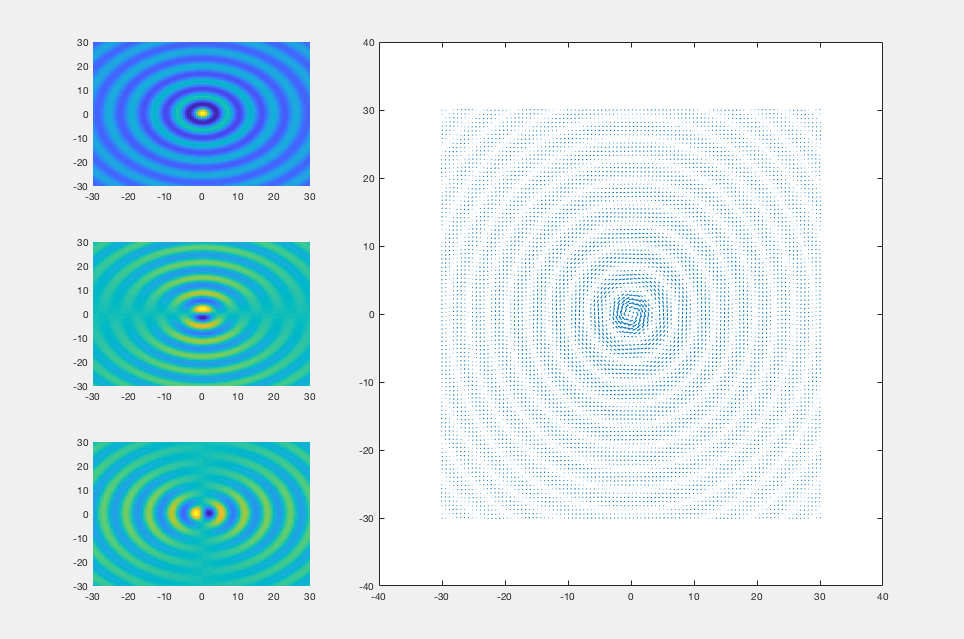
\includegraphics[width=1\columnwidth]{figures/JDipole}
}
\end{minipage}

\subsection{Magnetic Current Dipole: $J = [0,0,0]$ and $K = [0,K_y,0]$}
\begin{minipage}{0.5\textwidth}
\begin{align*}
    \mathcal{L}_1 K &= 
    \left[ \begin{array}{ccc} G & 0 & 0 \\ 
                            0 & G & 0\\ 
                            0 & 0 & G \end{array} \right]
        \left[ \begin{array}{c} 
        0 \\ K_y \\ 0 \end{array} \right]\\
    \mathcal{L}_2 K &= \frac{1}{k^2} \left[ \begin{array}{ccc} \frac{\partial^2 G }{\partial^2 x} & \frac{\partial^2 G }{\partial xy}\ & 0 \\ 
                            \frac{\partial^2 G}{\partial yx} & \frac{\partial^2 G}{\partial^2 y} &0\\ 
                            0 & 0 &0 \end{array} \right]
                                    \left[ \begin{array}{c} 
                            0 \\ K_y \\ 0 \end{array} \right]\\
    \ \\
    H^s &= -i\omega\epsilon \mathcal{L} K (\rho) \\ &= -i\omega\epsilon 
    \left( \left[ \begin{array}{ccc} G & 0 & 0 \\ 
                            0 & G & 0\\ 
                            0 & 0 & G \end{array} \right] + \frac{1}{k^2} \left[ \begin{array}{ccc} \frac{\partial^2 G }{\partial^2 x} & \frac{\partial^2 G }{\partial xy}\ & 0 \\ 
                            \frac{\partial^2 G}{\partial yx} & \frac{\partial^2 G}{\partial^2 y} &0\\ 
                            0 & 0 &0 \end{array} \right] \right)
        \left[ \begin{array}{c} 
        0 \\ K_y \\ 0 \end{array} \right]\\
         E^s &= \mathcal{R} K = \left[ \begin{array}{ccc} 0 & 0 & \frac{\partial G}{\partial y}\\ 
                            0 & 0 &-\frac{\partial G}{\partial x}\\ 
                            -\frac{\partial G}{\partial y} &\frac{\partial G}{\partial x} &0 \end{array} \right]
        \left[ \begin{array}{c} 
        0 \\ K_y \\ 0 \end{array} \right]\\
        \ \\
        H_y &= -i\omega\epsilon \left( G + \frac{1}{k^2}\frac{\partial^2 G}{\partial^2 y} \right) K_y, \quad  H_x = -i\omega\epsilon \frac{1}{k^2}\frac{\partial^2 G}{\partial xy} K_y, \quad E_z = \frac{dG}{dx} K_y
\end{align*}
\end{minipage}
\begin{minipage}{0.5\textwidth}
{\centering
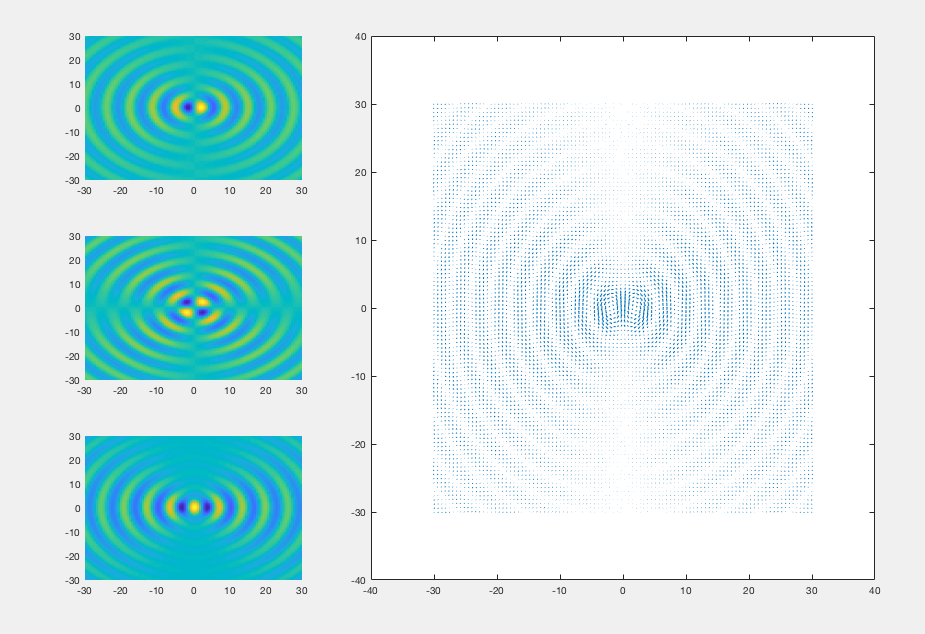
\includegraphics[width=1\columnwidth]{figures/KyDipole}
}
\end{minipage}

\subsection{Magnetic Current Dipole: $J = [0,0,0]$ and $K = [K_x,K_y,0]$}
\begin{minipage}{0.5\textwidth}
\begin{align*}
    \mathcal{L}_1 K &= 
    \left[ \begin{array}{ccc} G & 0 & 0 \\ 
                            0 & G & 0\\ 
                            0 & 0 & G \end{array} \right]
        \left[ \begin{array}{c} 
        K_x \\ K_y \\ 0 \end{array} \right]\\
    \mathcal{L}_2 K &= \frac{1}{k^2} \left[ \begin{array}{ccc} \frac{\partial^2 G }{\partial^2 x} & \frac{\partial^2 G }{\partial xy}\ & 0 \\ 
                            \frac{\partial^2 G}{\partial yx} & \frac{\partial^2 G}{\partial^2 y} &0\\ 
                            0 & 0 &0 \end{array} \right]
                                    \left[ \begin{array}{c} 
                            K_x \\ K_y \\ 0 \end{array} \right]\\
    \ \\
    H^s &= -i\omega\epsilon \mathcal{L} K (\rho) \\ &=-i\omega\epsilon 
    \left( \left[ \begin{array}{ccc} G & 0 & 0 \\ 
                            0 & G & 0\\ 
                            0 & 0 & G \end{array} \right] + \frac{1}{k^2} \left[ \begin{array}{ccc} \frac{\partial^2 G }{\partial^2 x} & \frac{\partial^2 G }{\partial xy}\ & 0 \\ 
                            \frac{\partial^2 G}{\partial yx} & \frac{\partial^2 G}{\partial^2 y} &0\\ 
                            0 & 0 &0 \end{array} \right] \right)
        \left[ \begin{array}{c} 
        K_x \\ K_y \\ 0 \end{array} \right]\\
         E^s &= \mathcal{R} K = \left[ \begin{array}{ccc} 0 & 0 & \frac{\partial G}{\partial y}\\ 
                            0 & 0 &-\frac{\partial G}{\partial x}\\ 
                            -\frac{\partial G}{\partial y} &\frac{\partial G}{\partial x} &0 \end{array} \right]
        \left[ \begin{array}{c} 
        K_x \\ K_y \\ 0 \end{array} \right]\\
        \ \\
        H_x &= -i\omega\epsilon \left[ \left( G + \frac{1}{k^2}\frac{\partial^2 G}{\partial^2 x} \right) K_x +
        \frac{1}{k^2}\frac{\partial^2 G}{\partial xy} K_y \right]\\
        H_y &= -i\omega\epsilon \left[ \frac{1}{k^2}\frac{\partial^2 G}{\partial yx} K_x +
        \left( G + \frac{1}{k^2}\frac{\partial^2 G}{\partial y^2} \right) K_y \right]\\
        E_z &= -\frac{dG}{dy} K_x + \frac{dG}{dx} K_y
\end{align*}
\end{minipage}
\begin{minipage}{0.5\textwidth}
{\centering
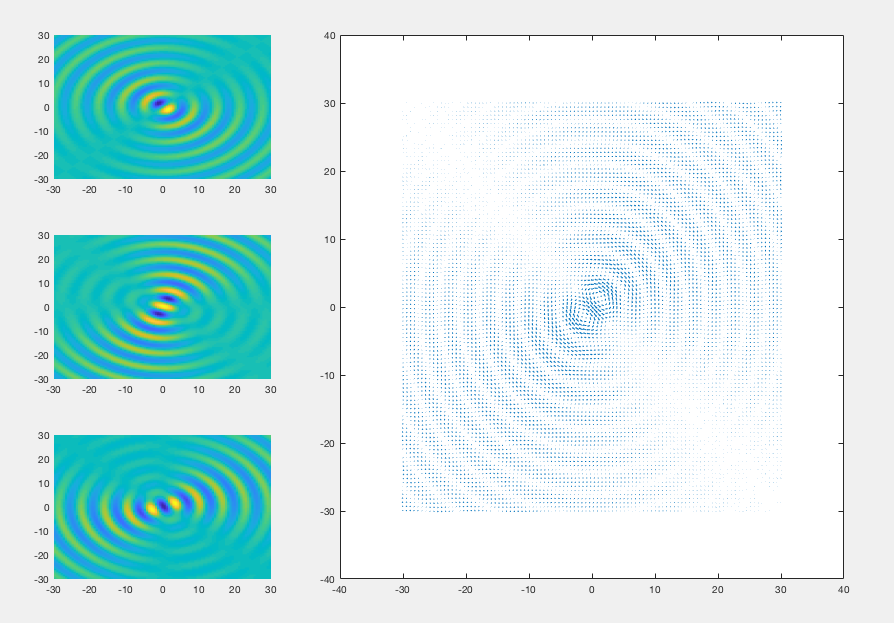
\includegraphics[width=1\columnwidth]{figures/KxyDipole}
}
\end{minipage}

\section{BEM Formulation for boundary: Metasurface and Dielectric}

\subsection{Original tjs/scott formulation}

For the BEM simulation we have $N_s$ double sided surfaces contained within $N_l$ loops. Over all the surfaces we have a total of $N_e$ surface elements. Each element has the unknowns:
\begin{align*}
    \begin{array}{ll}
    \J = [J_{x},J_{y},J_{z}] & \K = [K_{x},K_{y},K_{z}] \\
    \E_{1} = [E_{1x},E_{1y},E_{1z}] & \E_{2} = [E_{2x},E_{2y},E_{2z}] \\
    \H_{1} = [H_{1x},H_{1y},H_{1z}] & \H_{2} = [H_{2x},H_{2y},H_{2z}]
    \end{array}
\end{align*}
Therefore we have 6 sets of 3 vectors as unknowns over all of the surface elements. This gives a total of 18 unknowns per element.  

Now lets write down all the equations.

From the BEM loop formulation we will get 2 equations for all fields,
\begin{align} \label{Eq:BEMOper0}
\left.
\begin{array}{cc}
    \left[\begin{array}{c}\Ev_1\\\Ev_2\end{array}\right]
    = -j\omega\mu \SLm \Jv - \SRm \Kv & \quad
    \left[\begin{array}{c}\Hv_1\\\Hv_2\end{array}\right]
     = -j\omega\epsilon \SLm \Kv + \SRm \Jv
    \end{array}
    \right\}\quad\quad\text{2 $\times$ 6 = 12 equations}
\end{align}
Currents only on the surface so,
\begin{align} \label{Eq:CurrNormalDot}
\left.
    \begin{array}{cc}1
    \Jv \cdot \N = 0 & 
    \Kv \cdot \N = 0 \\
    \end{array}
 \right\}\quad\quad\text{2 $\times$ 1 =  2 equations}  
 \end{align}
 At each interface we expect constraints on the tangential fields. For a simple dielectric surface we will have,
\begin{align}\label{Eq:TangCont}
\left.
    \begin{array}{cc}
    \Ev^t_{1} = \Ev^t_{2} &
    \Hv^t_{1} = \Hv^t_{2} 
    \end{array}
 \right\}\quad\quad\text{2 $\times$ 3 =  6 equations}  
\end{align}
For an interfaces the normal component of the displacement fields ($\D$ and $\B$) are continuous, 
\begin{align}\label{Eq:NormalCont}
\left.
    \begin{array}{cc}
    \Ieps_1 \Ev^n_1  = \Ieps_2 \Ev^n_2 &
    \Imu_1 \Hv^n_1  = \Imu_2 \Hv^n_2
    \end{array}
    \right\}\quad\quad\text{2 $\times$ 3 =  6 equations}  
\end{align}
\subsubsection*{Vertical surface:}
For example with a vertical surface $\n = [1,0,0]$ and  
\begin{align*}
&\left.
    \begin{array}{c}
    \left[\begin{array}{c}\Ev_1\\\Ev_2\end{array}\right]
    = -j\omega\mu \SLm \Jv - \SRm \Kv\\\\
    \left[\begin{array}{c}\Hv_1\\\Hv_2\end{array}\right]
     = -j\omega\epsilon \SLm \Kv + \SRm \Jv
    \end{array}\right\} \quad \text{12 equations}\\
     &\left.
    \begin{array}{c}
    \Jv_x  = 0 \\
    \Kv_x = 0 
    \end{array}\quad \quad \quad \quad \quad \quad \right\} \quad \text{2 equations}\\
    &\left.
    \begin{array}{c}
    \left[\begin{array}{c}0\\\Ev_{y1}\\\Ev_{z1}\end{array}\right] = 
    \left[\begin{array}{c}0\\\Ev_{y2}\\\Ev_{z2}\end{array}\right] \\\\
    \left[\begin{array}{c}0\\\Hv_{y1}\\\Hv_{z1}\end{array}\right] = 
    \left[\begin{array}{c}0\\\Hv_{y2}\\\Hv_{z2}\end{array}\right] \\
    \end{array}\right\} \quad \text{4 equations}\\
    &\left.
    \begin{array}{c}
    \left[\begin{array}{c}\Ieps_1\Ev_{x1}\\0\\0\end{array}\right] = 
    \left[\begin{array}{c}\Ieps_2\Ev_{x2}\\0\\0\end{array}\right] \\\\
    \left[\begin{array}{c}\Imu_1\Hv_{x1}\\0\\0\end{array}\right] = 
    \left[\begin{array}{c}\Imu_2\Hv_{x2}\\0\\0\end{array}\right] \\
    \end{array}\right\} \quad \text{2 redundant equations}\\
\end{align*}
we have 20 equations and 18 unknowns. Choosing the surface current equations seems to work. Using the last set which matches the normal components does not work as the set of equations is not full rank. I assume the BEM operator equations include this set. 

\subsubsection*{General 2D Surface}
Surface is given by $\n = [n_x,n_y,0]$,
\begin{align*}
    \Phi \times n = 
    \begin{array}{|ccc|}
    \hat i & \hat j & \hat k\\
    \phi_x & \phi_y & \phi_z \\
        n_x & n_y & 0     
    \end{array}
    = 
    \left[
    \begin{array}{c}
        - \phi_z n_y\\
        \phi_z n_x \\
        \phi_x n_y - \phi_y n_x
    \end{array}
    \right]
\end{align*}
 and tangential components are,
\begin{align*}
    \Phi_t = \n \times (\Phi \times \n) = &\;\begin{array}{|ccc|}
    \hat i & \hat j & \hat k\\
    n_x & n_y & n_z     \\
    (\phi_y n_z - \phi_z n_y) & (\phi_z n_x - \phi_x n_z) & (\phi_x n_y - \phi_y n_x)
    \end{array}\\
    &= \left[
    \begin{array}{c}
     n_y (\phi_x n_y - \phi_y n_x) - n_z (\phi_z n_x - \phi_x n_z) \\
       n_z (\phi_y n_z - \phi_z n_y) - n_x (\phi_x n_y - \phi_y n_x)\\
       n_x (\phi_z n_x - \phi_x n_z) - n_y (\phi_y n_z - \phi_z n_y)
       \end{array} \right]
\end{align*}
but we want to specify,
\begin{align*}
    \begin{array}{c}
    \Ev^t_{1} = \Ev^t_{2} \\
    \Hv^t_{1} = \Hv^t_{2} 
    \end{array}  \rightarrow
    \begin{array}{c}
    \n \times (\Ev_1 \times \n) = \n \times (\Ev_2 \times \n)\\ 
    \n \times (\Hv_1 \times \n) = \n \times (\Hv_2 \times \n)
    \end{array} 
\end{align*}
and we can ignore the outer $\n \times$ operator,
\begin{align*}
    \begin{array}{c}
    \Ev^t_{1} = \Ev^t_{2} \\
    \Hv^t_{1} = \Hv^t_{2} 
    \end{array}  \rightarrow
    \begin{array}{c}
    \Ev_1 \times \n = \Ev_2 \times \n\\ 
    \Hv_1 \times \n = \Hv_2 \times \n
    \end{array} 
\end{align*}
This gives for example,
\begin{align*}
    \left[
    \begin{array}{c}
        - E_{1z} n_y\\
        E_{1z} n_x \\
        E_{1x} n_y - E_{1y} n_x
    \end{array}
    \right] = 
       \left[
    \begin{array}{c}
        - E_{2z} n_y\\
        E_{2z} n_x \\
        E_{1x} n_y - E_{1y} n_x
    \end{array} 
    \right]
\end{align*}
The first two equations are equivalent and simple specify the continuity of $E_z$ a tangential component by definition. We need to replace one of them with the surface current constraint. I propose we use,
\begin{align*}
    \left[
    \begin{array}{c}
        E_{1z}\\
        E_{1x} n_y - E_{1y} n_x
    \end{array}
    \right] = 
       \left[
    \begin{array}{c}
        E_{2z} \\
        E_{1x} n_y - E_{1y} n_x
    \end{array} 
    \right]
\end{align*}
which should be well behaved.

Therefore we have as our equations,
\begin{align*}
&\left.
    \begin{array}{c}
    \left[\begin{array}{c}\Ev_1\\\Ev_2\end{array}\right]
    = -j\omega\mu \SLm \Jv - \SRm \Kv\\\\
    \left[\begin{array}{c}\Hv_1\\\Hv_2\end{array}\right]
     = -j\omega\epsilon \SLm \Kv + \SRm \Jv
    \end{array}\right\} \quad \text{12 equations}\\
     &\left.
    \begin{array}{c}
    \Jv_x \N_x + \Jv_y \N_y  = 0 \\
    \Kv_x \N_x + \Kv_y \N_y = 0 
    \end{array}\quad \quad \quad \quad \quad \quad \right\} \quad \text{2 equations}\\
    & \left.
     \begin{array}{c}
    \left[
    \begin{array}{c}
        \Ev_{1z} \\
        \Ev_{1x} \N_y - \Ev_{1y} \N_x
    \end{array}
    \right] = 
       \left[
    \begin{array}{c}
        \Ev_{2z} \\
        \Ev_{1x} \N_y - \Ev_{1y} \N_x
    \end{array} \right] \\\\
    \left[
    \begin{array}{c}
        \Hv_{1z} \\
        \Hv_{1x} \N_y - \Hv_{1y} \N_x
    \end{array}
    \right] = 
       \left[
    \begin{array}{c}
        \Hv_{2z} \\
        \Hv_{1x} \N_y - \Hv_{1y} \N_x
    \end{array} \right] 
    \end{array}
    \quad \quad \quad \quad \quad \quad \right\} \quad \text{4 equations}\\
\end{align*}
which is 18 equations.

% \subsection{Independent component formulation}
% For the BEM simulation we have $N_s$ double sided surfaces contained within $N_l$ loops. Over all the surfaces we have a total of $N_e$ surface elements. Each element has the unknowns:
% \begin{align*}
%   \begin{array}{lll}
%   \J = [J_{x},J_{y},J_{z}] & \K = [K_{x},K_{y},K_{z}] &\\
%   \E_{1} = [E_{1x},E_{1y},E_{1z}] & \E^t_{1} = [E^t_{1x},E^t_{1y},E^t_{1z}] & \E^n_{1} =  [E^n_{1x},E^n_{1y},E^n_{1z}]\\
%   \E_{2} = [E_{2x},E_{2y},E_{2z}] & \E^t_{2} = [E^t_{2x},E^t_{2y},E^t_{2z}] & \E^n_{2}  =  [E^n_{2x},E^n_{2y},E^n_{2z}]\\
%   \H_{1} = [H_{1x},H_{1y},H_{1z}] & \H^t_{1} = [H^t_{1x},H^t_{1y},H^t_{1z}] &  \H^n_{1} =  [H^n_{1x},H^n_{1y},H^n_{1z}]\\ 
%   \H_{2} = [H_{2x},H_{2y},H_{2z}] & \H^t_{2} = [H^t_{2x},H^t_{2y},H^t_{2z}] & \H^n_{2} =  [H^n_{2x},H^n_{2y},H^n_{2z}]
%   \end{array}
% \end{align*}
% where we have decomposed each field at the surface to have independent normal ($\Phi^n$) and tangential ($\Phi^t$) components. Therefore we have 14 sets of 3 vectors as unknowns over all of the surface elements. This gives a total of 42 unknowns per element.  

% Now lets write down all the equations. The field decomposition for all elements can be expressed as 4 vector equations each of 3 components,
% \begin{align}\label{Eq:FieldDecomp}
%   \left.
%   \begin{array}{cc}
%   \Ev_{1} = \Ev^t_{1} + \Ev^n_{1}&
%   \Ev_{2} = \Ev^t_{2} + \Ev^n_{2}\\
%   \Hv_{1} = \Hv^t_{1} + \Hv^n_{1}&
%   \Hv_{2} = \Hv^t_{2} + \Hv^n_{2}
%   \end{array}
%   \right\}\quad\quad\text{4 $\times$ 3 = 12 equations}
% \end{align}
% From the BEM loop formulation we will get 2 equations for all fields,
% \begin{align} \label{Eq:BEMOper}
% \left.
% \begin{array}{cc}
%   \left[\begin{array}{c}\Ev_1\\\Ev_2\end{array}\right]
%   = -j\omega\mu \SLm \Jv - \SRm \Kv & \quad
%   \left[\begin{array}{c}\Hv_1\\\Hv_2\end{array}\right]
%    = -j\omega\epsilon \SLm \Kv + \SRm \Jv
%   \end{array}
%   \right\}\quad\quad\text{2 $\times$ 6 = 12 equations}
% \end{align}
% Tangential fields are only on the surface so we have 4 more equations,
% \begin{align} \label{Eq:FieldNormalDot}
% \left.
%   \begin{array}{cc}
%   \Ev^t_1 \cdot \N = 0 &
%   \Ev^t_2 \cdot \N = 0\\
%   \Hv^t_1 \cdot \N = 0 &
%   \Hv^t_2 \cdot \N = 0
%   \end{array}
% \right\}\quad\quad\text{4 $\times$ 1 =  4 equations}
% \end{align}
% and normal component must be normal so 4 vector equations,
% \begin{align} \label{Eq:FieldNormalCross}
% \left.
%   \begin{array}{cc}
%   \Ev^n_1 \times \N = \0 &
%   \Ev^n_2 \times \N = \0 \\
%   \Hv^n_1 \times \N = \0 &
%   \Hv^n_2 \times \N = \0
%     \end{array}
%  \right\}\quad\quad\text{4 $\times$ 3 =  12 equations}  
%  \end{align}
% At each interface we expect constraints on the tangential fields. For a simple dielectric surface we will have,
% \begin{align}\label{Eq:TangCont}
% \left.
%   \begin{array}{cc}
%   \Ev^t_{1} = \Ev^t_{2} &
%   \Hv^t_{1} = \Hv^t_{2} 
%   \end{array}
%  \right\}\quad\quad\text{2 $\times$ 3 =  6 equations}  
% \end{align}
% % where as for a metasurface:
% % \begin{align*}
% %   \DE_{t}  &= j \omega \chi_e  \Hb_t \times \n \\
% %   \DH_{t}  &= j \omega \chi_m  \Eb_t \times \n 
% % \end{align*}
% Currents only on the surface so,
% \begin{align} \label{Eq:CurrNormalDot}
% \left.
%   \begin{array}{cc}
%   \Jv \cdot \N = 0 & 
%   \Kv \cdot \N = 0 \\
%   \end{array}
%  \right\}\quad\quad\text{2 $\times$ 1 =  2 equations}  
% \end{align}
% For both both interfaces the normal component of the displacement fields ($\D$ and $\B$) are continuous, 
% \begin{align}\label{Eq:NormalCont}
% \left.
%   \begin{array}{cc}
%   \Ieps_1 \Ev^n_1  = \Ieps_2 \Ev^n_2 &
%   \Imu_1 \Hv^n_1  = \Imu_2 \Hv^n_2
%   \end{array}
%   \right\}\quad\quad\text{2 $\times$ 3 =  6 equations}  
% \end{align}
% This gives $12+12+4+12+6+2+6 = 52$ equations for 42 unknowns. 


% However, I think that \refeq{Eq:CurrNormalDot} (current constraint equation) is redundant as 
% % , but I think that \eqref{Eq:NormalCross} is redundant as \eqref{Eq:NormalDot} specifies that the tangential component is actually tangential and the ``remainder'' must be normal. This would give 24 equations and 24 unknowns for each segment.


% \subsubsection*{Vertical surface:}
% For example with a vertical surface $\n = [1,0,0]$ and  
% \begin{align*}
% \Phi \cdot \n &= \phi_x \\
% \Phi \times \n &= (\phi_y n_z - \phi_z n_y) \hat i + (\phi_z n_x - \phi_x n_z) \hat j + (\phi_x n_y - \phi_y n_x) \hat k\\
%              & = 0 \hat i + \phi_z  \hat j - \phi_y \hat k\\
% \end{align*}
% we have
% \begin{align*}
%   &\left.
%   \begin{array}{c}
%   \Ev_{1} = \Ev^t_{1} + \Ev^n_{1}\\
%   \Ev_{2} = \Ev^t_{2} + \Ev^n_{2}\\
%   \Hv_{1} = \Hv^t_{1} + \Hv^n_{1}\\
%   \Hv_{2} = \Hv^t_{2} + \Hv^n_{2}
%   \end{array} \quad 
%   \begin{array}{c}
%   \left[\begin{array}{c}\Ev_1\\\Ev_2\end{array}\right]
%   = -j\omega\mu \SLm \Jv - \SRm \Kv\\\\
%   \left[\begin{array}{c}\Hv_1\\\Hv_2\end{array}\right]
%    = -j\omega\epsilon \SLm \Kv + \SRm \Jv
%   \end{array}\right\} \quad \text{24 equations}\\
%   &\left.
%   \begin{array}{c}
%   \Ev^t_{x1}  = 0 \\
%   \Ev^t_{x2}  = 0 \\
%   \Hv^t_{x1}  = 0 \\
%   \Hv^t_{x2}  = 0 
%   \end{array}\right\} \quad \text{4 equations}\\
%   \begin{array}{c}
%   \Ev^n_1 \times \N = \0\\
%   \Ev^n_2 \times \N = \0\\
%   \Hv^n_1 \times \N = \0\\
%   \Hv^n_2 \times \N = \0
%     \end{array} \longrightarrow&  \left.
%     \left[\begin{array}{c}0\\\Ev^n_{1z}\\\Ev^n_{1y}\end{array}\right]
%     = \left[\begin{array}{c}0\\0\\0\end{array}\right]\quad
%       \left[\begin{array}{c}0\\\Ev^n_{2z}\\\Ev^n_{2y}\end{array}\right]
%     = \left[\begin{array}{c}0\\0\\0\end{array}\right]\quad
%       \left[\begin{array}{c}0\\\Hv^n_{1z}\\\Hv^n_{1y}\end{array}\right]
%     = \left[\begin{array}{c}0\\0\\0\end{array}\right]\quad
%       \left[\begin{array}{c}0\\\Hv^n_{2z}\\\Hv^n_{2y}\end{array}\right]
%     = \left[\begin{array}{c}0\\0\\0\end{array}\right]\quad\right\} \quad \text{8 equations}\\
%     &\left.
%     \begin{array}{c}
%   \Ev^t_{1} = \Ev^t_{2}\\
%   \Hv^t_{1} = \Hv^t_{2}
%   \end{array}\right\} \quad \text{6 equations}\\
%     &\left.
%     \begin{array}{c}
%   \Jv_x  = 0 \\
%   \Kv_x = 0 
%   \end{array}\right\} \quad \text{2 redundant equations}\\
%     &\left.
%     \begin{array}{c}
%   \Ieps_1 \Ev^n_1  = \Ieps_2 \Ev^n_2\\
%   \Imu_1 \Hv^n_1  = \Imu_2 \Hv^n_2 
%   \end{array}\right\} \quad \text{6 redundant equations}\\
% \end{align*}
% This gives us $24+4+8+6 = 42$ equations for 42 unknowns.

% We can arrange these into a solution over all surface elements as:
% \begin{align*}
% \left[
%     \begin{array}{cccccccccc}
%     j\omega\mu\SLm &\SRm  & \0 & \0 & \0 & \0 & \I & \0 \\
%     -\SRm & j\omega\epsilon\SLm  & \0 & \0 & \0 & \0 & \0 & \I \\
%     \0 & \0 & \0 & \0 & \N & \Chibb_\text{m} & -\N & \Chibb_\text{m} & \0 & \0 \\
%     \0 & \0 & \0 & \0 & -\Chibb_\text{e} & \N & -\Chibb_\text{e} & -\N & \0 & \0 \\
%     \0 & \0 & \0 & \0 & \0 & \0 & \0 & \0 & \I & \0 \\
%     \0 & \0 & \0 & \0 & \0 & \0 & \0 & \0 & \0 & \I \\
%     \end{array}
% \right]
% \left[
%     \begin{array}{c}
%     \Jv\\ \Kv \\ \Ev^t_1\\ \Ev^n_1\\\Hv^t_1\\\Hv^n_1\\\Ev^t_2\\ \Ev^n_2\\\Hv^t_2\\\Hv^n_2\\
%     \end{array}
% \right] 
% = 
% \left[
%     \begin{array}{c}
%     \0\\ \0\\ \0 \\ \0 \\ \0 \\ \0 \\ \0 \\ \0  \\ \Ev_0 \\ \Hv_0
%     \end{array}
% \right] \nonumber
% \end{align*}

% \begin{equation}
% \Sm \Ym = \Bm \label{Eq:TwoRegScat}
% \end{equation}

\section{Surface Equations}

\begin{figure}[htbp]
\begin{center}
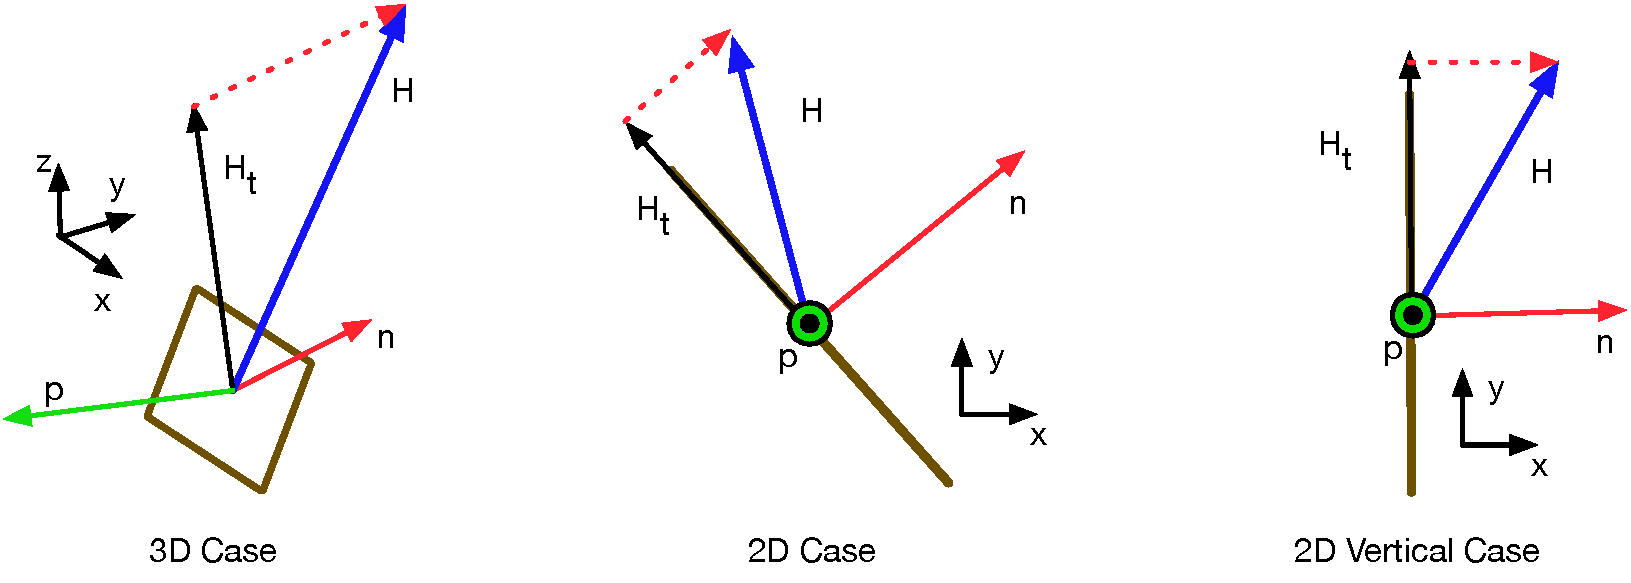
\includegraphics[width=1\columnwidth]{figures/SurfGeo}
\caption{$\Hb = [H_x,H_y,H_z]$ is the average field present at surface. $\n = [nx,ny,nz]$ is direction vector normal to surface element. $\Ht$ is field component tangential to surface. $p$ is orthogonal to both $n$ and $t$ and lies in the plane of the surface element.}\label{Fig:Surface Geo}
\end{center}
\end{figure}


For a metasurface at the point (x,y,z) on the surface with a normal $\n(x,y,z$ we have 4 fields:
\begin{align*}
\begin{array}{cc}
    \E_1 & \text{-- E field in region 1 adjacent to the surface}\\
    \E_2 & \text{-- E field in region 2 adjacent to the surface}\\
    \H_1 & \text{-- H field in region 1 adjacent to the surface}\\
    \H_2 & \text{-- H field in region 2 adjacent to the surface}
\end{array}
\end{align*}
we can decompose each field ($\Phi$) into a tangential component ($\Phi_t$) in the surface plane and one normal to it ($\Phi_n$),
\begin{align*}
\Phi_t &= \n \times (\Phi \times \n) \\
\Phi_n &= \n \cdot \Phi
\end{align*}
and for example $\E_1 = \E_{1t} + \E_{1n}$.

The GSTC's express a relationship between the tangential components of the $\E$ and $\H$ fields,
\begin{align*}
    \E_{1t} - \E_{2t}  &= j \omega \chi \frac{\H_{1t} + \H_{2t}}{2} \times \n\\
    \DE_{t}  &= j \omega \chi  \Hb_t \times \n\\
\end{align*}
where as we know that $\Hb_t$ is orthogonal to $\n$ by construction. Therefore $\DE_{t}$ will be orthogonal to both $\Hb_1$ and $\n$ and in the plane of the surface. 

We also know that the $\DE$ in the direction of $\H_{t}$ will be equal to zero as that is perpendicular to the tangential field created by the metasurface,
\begin{align*}
\DE \cdot \frac{\Hb_t}{|\Hb_t|} = 0
\end{align*}

\newpage
and $\Hb = [H_x H_y H_z]$,
\begin{align*}
    \Hb \times n = 
    \begin{array}{|ccc|}
    \hat i & \hat j & \hat k\\
    H_x & H_y & H_z \\
        n_x & n_y & n_z     
    \end{array}
    = (H_y n_z - H_z n_y) \hat i + (H_z n_x - H_x n_z) \hat j + (H_x n_y - H_y n_x) \hat k
\end{align*}

\begin{align*}
    \Hb_t = \n \times (\Hb \times \n) = &\;\begin{array}{|ccc|}
    \hat i & \hat j & \hat k\\
    n_x & n_y & n_z     \\
    (H_y n_z - H_z n_y) & (H_z n_x - H_x n_z) & (H_x n_y - H_y n_x)
    \end{array}\\
     = &\left[n_y (H_x n_y - H_y n_x) - n_z (H_z n_x - H_x n_z) \right] \hat i \;\; + \\
       &\left[n_z (H_y n_z - H_z n_y) - n_x (H_x n_y - H_y n_x)\right] \hat j \;\; + \\
       &\left[n_x (H_z n_x - H_x n_z) - n_y (H_y n_z - H_z n_y) \right] \hat k
\end{align*}

If 2D then: $n = n_{xy} = [nx,ny,0]$,
\begin{align*}
    \n \times (\Hb \times \n) 
     = &\left[n_y (H_x n_y - H_y n_x) \right] \hat i \;\; + \\
       &\left[ - n_x (H_x n_y - H_y n_x)\right] \hat j \;\; + \\
       &\left[n_x H_z n_x + n_y  H_z n_y \right] \hat k
\end{align*}
If $H_z = 0$ TEM, 
\begin{align*}
    \n \times (\Hb \times \n) 
     = &\left[n_y (H_x n_y - H_y n_x) \right] \hat i \;\; + \\
       &\left[ - n_x (H_x n_y - H_y n_x)\right] \hat j \;\; + \\
       &\left[0 \right] \hat k
\end{align*}
If vertical $n_y = 0$ and $n_x = 1$
\begin{align*}
    \n \times (\Hb \times \n) 
     = &\left[0 \right] \hat i + 
       \left[ + n_x^2 H_y \right] \hat j \;\; + 
       \left[0 \right] \hat k\\
       == &\left[0 \right] \hat i + 
       \left[ +  H_y \right] \hat j \;\; + 
       \left[0 \right] \hat k\\    
\end{align*}

\begin{align*}
     \Hb_t \times \n &= \left[
     \begin{array}{c}
     n_y (H_x n_y - H_y n_x) - n_z (H_z n_x - H_x n_z)\\
     n_z (H_y n_z - H_z n_y) - n_x (H_x n_y - H_y n_x)\\
     n_x (H_z n_x - H_x n_z) - n_y (H_y n_z - H_z n_y) 
     \end{array}
     \right] \times \n\\\\
     & =     
     \begin{array}{|ccc|}
        \hat i & \hat j & \hat k\\      
     n_y (H_x n_y - H_y n_x) - n_z (H_z n_x - H_x n_z) &
     n_z (H_y n_z - H_z n_y) - n_x (H_x n_y - H_y n_x) &
     n_x (H_z n_x - H_x n_z) - n_y (H_y n_z - H_z n_y) \\
        n_x & n_y & n_z \\
    \end{array}\\\\
    &=  \left[
    \begin{array}{c}
    [n_z (H_y n_z - H_z n_y) - n_x (H_x n_y - H_y n_x)] n_z - [n_x (H_z n_x - H_x n_z) - n_y (H_y n_z - H_z n_y)] n_y\\
    -[n_y (H_x n_y - H_y n_x) - n_z (H_z n_x - H_x n_z)] n_z + [n_x (H_z n_x - H_x n_z) - n_y (H_y n_z - H_z n_y)]n_x\\
    +[n_y (H_x n_y - H_y n_x) - n_z (H_z n_x - H_x n_z)] n_y - [n_z (H_y n_z - H_z n_y) - n_x (H_x n_y - H_y n_x)]n_x
    \end{array} \right]
\end{align*}

2D ($n_z = 0$) and $Hz = 0$ 
\begin{align*}
    \Hb_t \times \n &=  \left[
    \begin{array}{c}
    [0 (H_y n_z - 0 n_y) - n_x (H_x n_y - H_y n_x)] 0 - [n_x (0 n_x - H_x 0) - n_y (H_y 0 - 0 n_y)] n_y\\
    -[n_y (H_x n_y - H_y n_x) - 0 (0 n_x - H_x 0)] 0 + [n_x (0 n_x - H_x 0) - n_y (H_y 0 - 0 n_y)]n_x\\
    +[n_y (H_x n_y - H_y n_x) - 0 (0 n_x - H_x 0)] n_y - [0 (H_y n_z - 0 n_y) - n_x (H_x n_y - H_y n_x)]n_x
    \end{array} \right]\\\\
    &=  \left[
    \begin{array}{c}
     - [ - n_y ( - 0 n_y)] n_y\\
     + [0] n_x\\
    +[n_y (H_x n_y - H_y n_x)] n_y - [ - n_x (H_x n_y - H_y n_x)]n_x
    \end{array} \right]\\    
    &=  \left[
    \begin{array}{c}
     - 0\\
     + 0\\
    +[(H_x n_y - H_y n_x)] n^2_y + [(H_x n_y - H_y n_x)]n^2_x
    \end{array} \right] = \left[
    \begin{array}{c}
     - 0\\
     + 0\\
    +(H_x n_y - H_y n_x)(n^2_y+ n^2_x)
    \end{array} \right]\\
    &=  \left[
    \begin{array}{c}
     0\\
     0\\
    +(H_x n_y - H_y n_x)
    \end{array} \right]
\end{align*}
and vertical surface ($n_y = 0$, $n_x = 1$)
\begin{align*}
    \Hb_t \times \n &=  \left[
    \begin{array}{c}
     0\\
     0\\
    - H_y
    \end{array} \right]
\end{align*}

\newpage
For the metasurface,
\begin{align*}
    \Delta \E_p &= j \omega \chi\; \Ht \times \n\\
\end{align*}
2D ($n_z = 0$) and $Hz = 0$:
\begin{align*}
    \left[
    \begin{array}{c}
     \dE_x\\
     \dE_y\\
     \dE_z 
     \end{array} \right]
  &= j \omega \chi \left[
    \begin{array}{c}
     0\\
     0\\
    H_x n_y - H_y n_x
    \end{array} \right]
\end{align*}
and vertical surface,
\begin{align*}
    \left[
    \begin{array}{c}
     \dE_x\\
     \dE_y\\
     \dE_z
     \end{array} \right]
  &= j \omega \chi \left[
    \begin{array}{c}
     0\\
     0\\
    - H_y
    \end{array} \right]
\end{align*}
other metasurface equations will give likewise,
\begin{align*}
    \left[
    \begin{array}{c}
     \dH_x\\
     \dH_y\\
     \dH_z
     \end{array} \right]
  &= j \omega \chi \left[
    \begin{array}{c}
     0\\
     0\\
    E_x n_y - E_y n_x
    \end{array} \right]
\end{align*}
and vertical surface,
\begin{align*}
    \left[
    \begin{array}{c}
     \dH_x\\
     \dH_y\\
     \dH_z
     \end{array} \right]
  &= j \omega \chi \left[
    \begin{array}{c}
     0\\
     0\\
    - E_y
    \end{array} \right]
\end{align*}


Previous formulation:
\begin{align*}
    \n \times \Delta \H = -j \omega \chi\Eb
\end{align*}
gives,
\begin{align*}
    \n \times \DE = &\;\begin{array}{|ccc|}
    \hat i & \hat j & \hat k\\
    n_x & n_y & n_z     \\
     \dH_x& \dH_y & \dH_z
    \end{array}\\
     = &\left[n_y \dH_z - n_z \dH_y \right] \hat i \;\; + 
       \left[-n_x \dH_z + n_z \dH_x\right] \hat j \;\; + 
       \left[n_x \dH_y - n_y \dH_x\right] \hat k
\end{align*}

\begin{align*}
    \left[
    \begin{array}{c}
    n_y \dH_z - n_z \dH_y\\ 
    -n_x \dH_z + n_z \dH_x\\
    n_x \dH_y - n_y \dH_x
    \end{array} \right] = 
    -j \omega \chi 
    \left[
    \begin{array}{c}
     E_x\\
     E_y\\
     E_z
     \end{array} \right]
     \xrightarrow{2D/TEM/vert}
    \left[
    \begin{array}{c}
    0\\ 
    -\dH_z\\
    \dH_y
    \end{array} \right] = 
    -j \omega \chi 
    \left[
    \begin{array}{c}
     E_x\\
     E_y\\
     E_z
     \end{array} \right]
\end{align*}

\begin{align*}
    \n \times \Delta \E = -j \omega \chi\Hb
\end{align*}
gives,
\begin{align*}
    \n \times \DE = &\;\begin{array}{|ccc|}
    \hat i & \hat j & \hat k\\
    n_x & n_y & n_z     \\
     \dE_x& \dE_y & \dE_z
    \end{array}\\
     = &\left[n_y \dE_z - n_z \dE_y \right] \hat i \;\; + 
       \left[-n_x \dE_z + n_z \dE_x\right] \hat j \;\; + 
       \left[n_x \dE_y - n_y \dE_x\right] \hat k
\end{align*}

\begin{align*}
    \left[
    \begin{array}{c}
    n_y \dE_z - n_z \dE_y\\ 
    -n_x \dE_z + n_z \dE_x\\
    n_x \dE_y - n_y \dE_x
    \end{array} \right] = 
    -j \omega \chi 
    \left[
    \begin{array}{c}
     H_x\\
     H_y\\
     H_z
     \end{array} \right]
     \xrightarrow{2D/TEM/vert}
    \left[
    \begin{array}{c}
    0\\ 
    -\dE_z\\
    \dE_y
    \end{array} \right] = 
    -j \omega \chi 
    \left[
    \begin{array}{c}
     H_x\\
     H_y\\
     H_z
     \end{array} \right]
\end{align*}


\subsection{Field Configurations for Constant $J_z$ and $K_y$}
\begin{minipage}{0.55\textwidth}
\begin{center}
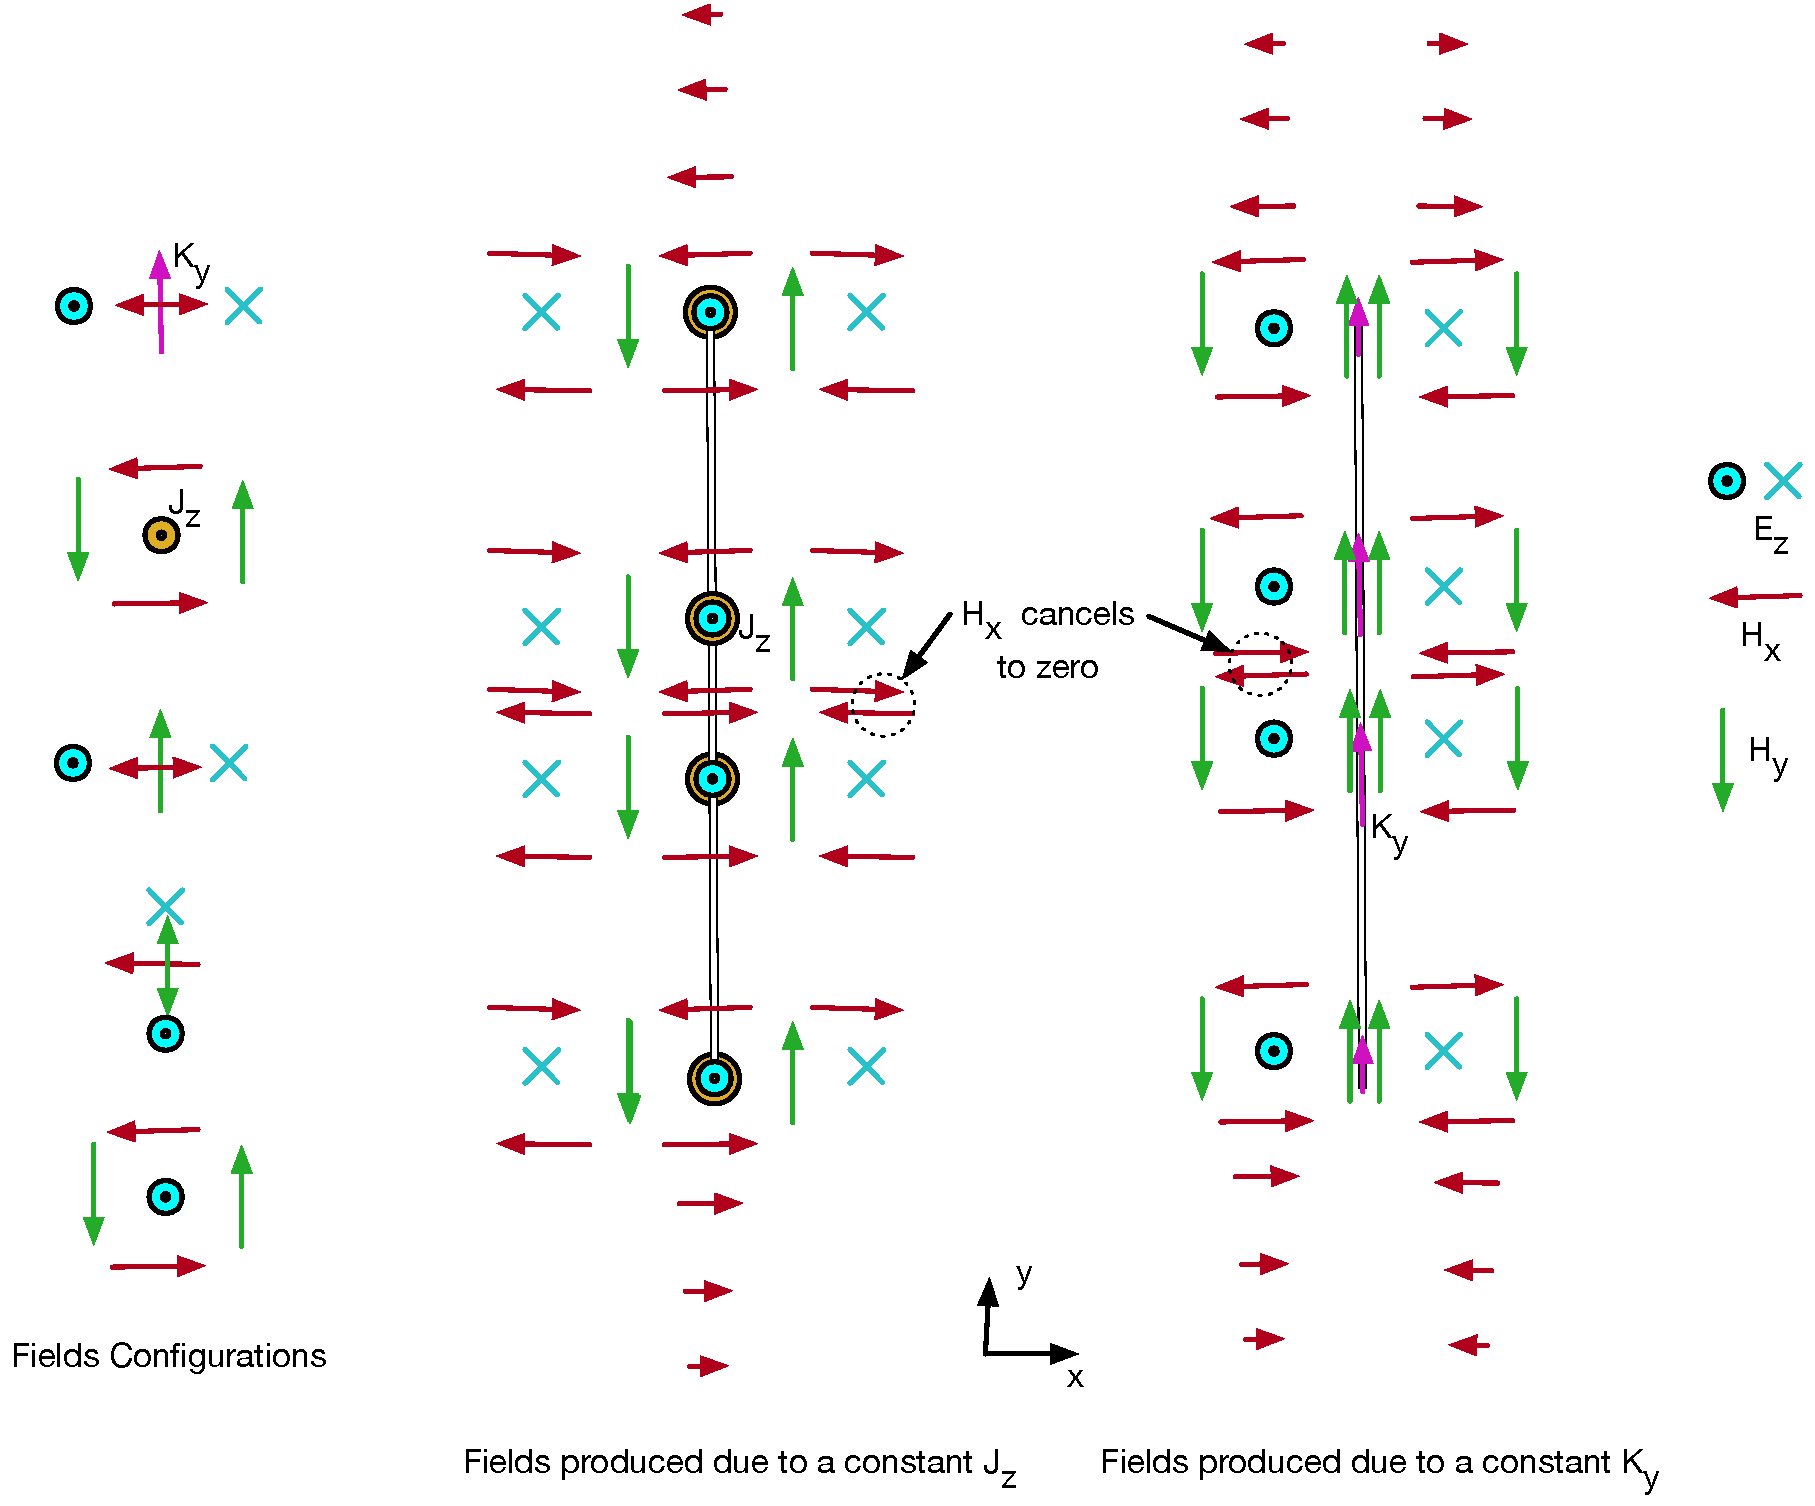
\includegraphics[width=1\columnwidth]{figures/FieldsSeg}
\end{center}
\end{minipage}
\begin{minipage}{0.45\textwidth}
\begin{align*}
\nabla \cdot E = 0 \quad \quad
& \nabla \cdot H = 0 \\
\nabla \times E = -\mu \frac{\partial H}{dt} + K\quad \quad 
& \nabla \times H = -\epsilon \frac{\partial E}{dt} + J
\end{align*}
Due to the infinite projection in z the fields generated ``above'' or below the current are ``canceled'' by complementary sources in along z. 
    \begin{enumerate}
        \item $H_x$ from a $K_y$ are not present.
        \item $H_x$ from a $H_y$ are not present.
        \item $H_y$ from a $H_x$ are not present.
    \end{enumerate}
\begin{align*}
    E^s(\rho) &= -i\omega\mu(\mathcal{L}J_s)(\rho) - (\mathcal{R}K_s)(\rho)\\
    H^s(\rho) &= -i\omega\epsilon(\mathcal{L}K_s)(\rho) + (\mathcal{R}J_s)(\rho)
\end{align*}
\begin{align*}
    (\mathcal{L}J)(\rho) &= \int_{\ell}G(\rho,\rho')[1+\frac{1}{k^2}\nabla'\nabla'\cdotp]J(\rho') \,d\rho'\\
    (\mathcal{R}J)(\rho) &= \nabla \times \int_{\ell}G(\rho,\rho')J(\rho') \,d\rho'\\
    (\mathcal{L}K)(\rho) &= \int_{\ell}G(\rho,\rho')[1+\frac{1}{k^2}\nabla'\nabla'\cdotp]K(\rho') \,d\rho'\\
    (\mathcal{R}K)(\rho) &= \nabla \times \int_{\ell}G(\rho,\rho')K(\rho') \,d\rho'
\end{align*}
\end{minipage}
\begin{minipage}{0.55\textwidth}
\begin{center}
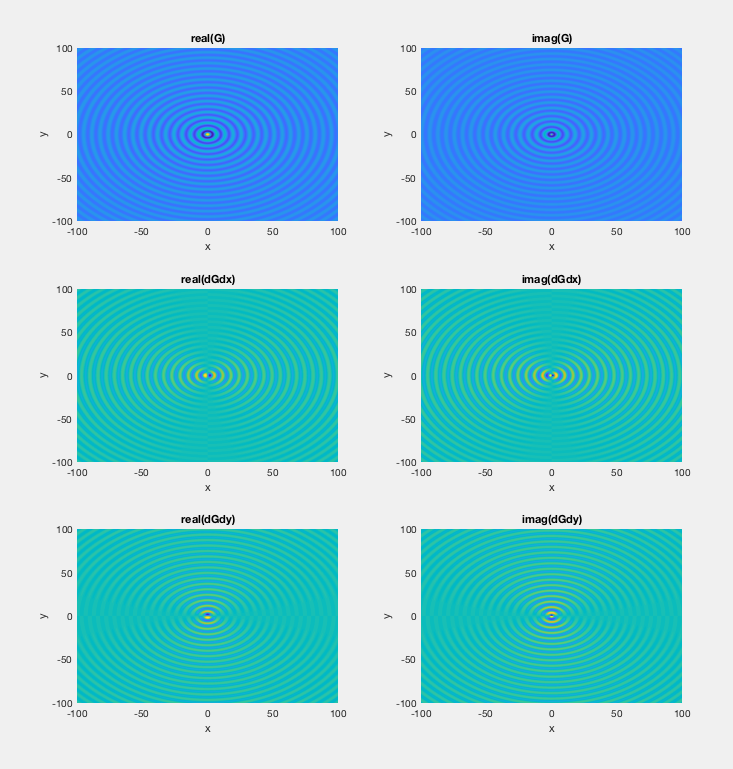
\includegraphics[width=0.75\columnwidth]{figures/GFct}
\end{center}
\end{minipage}
\begin{minipage}{0.45\textwidth}
\begin{align*}
    G(x, y, x', y') &= -\frac{i}{4}H_0^{(2)}(k\sqrt{(x-x')^2+(y-y')^2})\\
    \frac{\partial G}{\partial y'} &= -\frac{i}{4}\frac{k(y-y')H_1^{(2)}(k|\rho-\rho'|)}{|\rho-\rho'|}\\
    \frac{\partial G}{\partial x'} &= -\frac{i}{4}\frac{k(x-x')H_1^{(2)}(k|\rho-\rho'|)}{|\rho-\rho'|}
\end{align*}
\begin{enumerate}
    \item $G$ is symmetrical in both $x$ and $y$.
    \item $\partial G/ \partial x$ is anti-symmetrical in  $x$ and symmetrical in $y$.
    \item $\partial G/ \partial y$ is symmetrical in $x$ and anti-symmetrical in $y$.
\end{enumerate}
\end{minipage}
\newpage

\subsubsection*{Expected fields from Maxwell's equations:}

\noindent {\bf Only a constant $J_z$ in surface:}

\begin{minipage}{0.45\textwidth}
\begin{center}
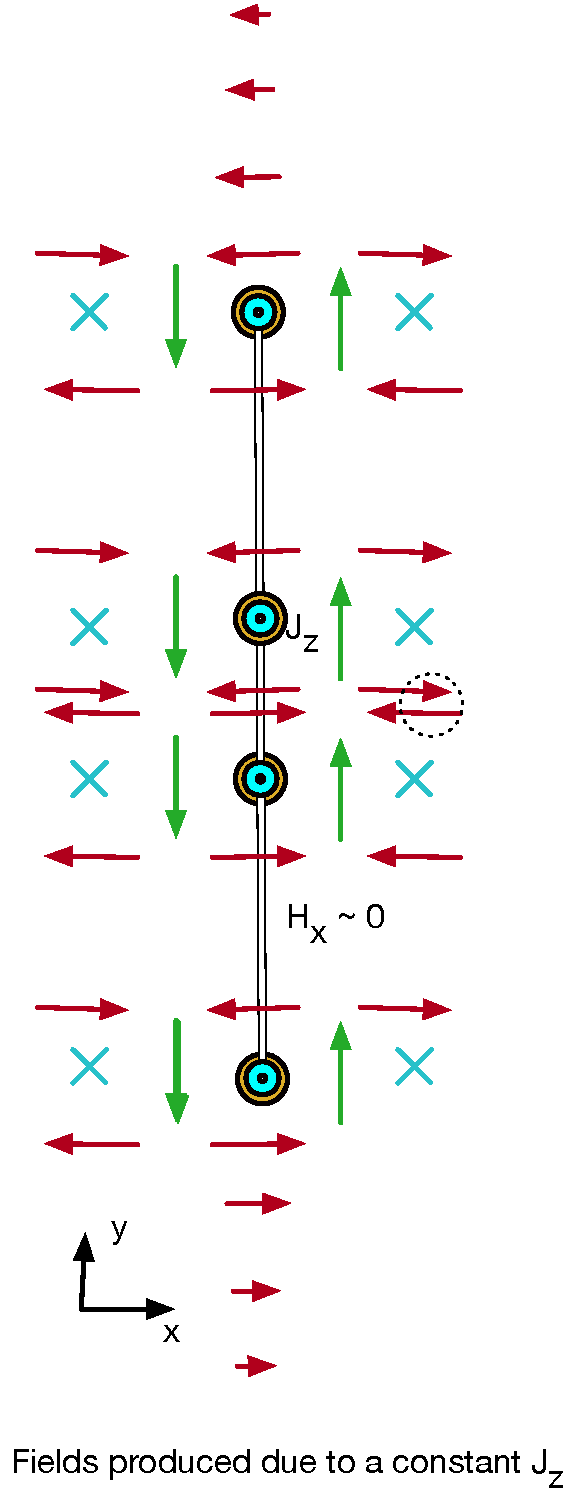
\includegraphics[width=0.24\columnwidth]{figures/OnlyJs}
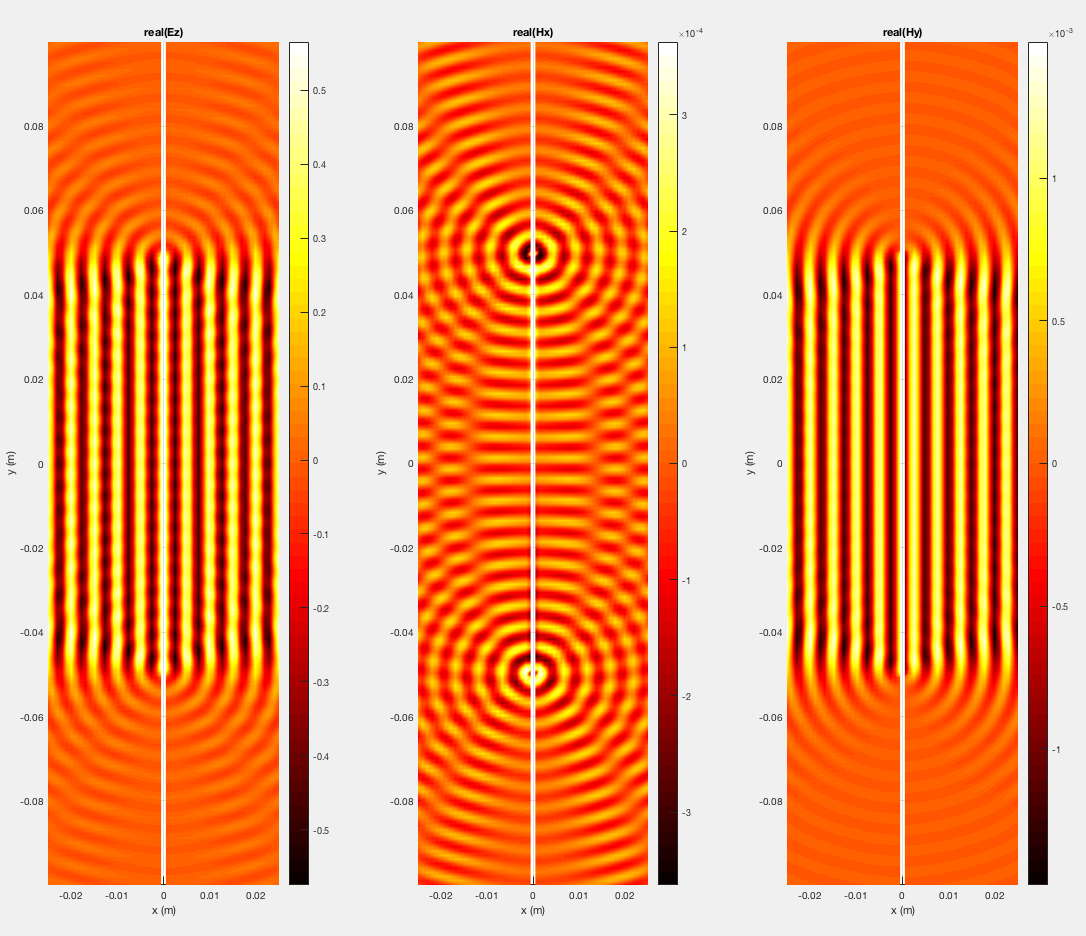
\includegraphics[width=0.74\columnwidth]{figures/OnlyJsZeroDerv.png}
\end{center}
\end{minipage}
\begin{minipage}{0.45\textwidth}
Near middle of segment we have plane-wave ($E_x, H_y$) like fields. 
\begin{enumerate}
    \item Isolated harmonic $J_z$ creates both $H_x$ and $H_y$ fields.
    \item In the center of the surface the $H_x$ field is mainly ``canceled'' due to anti-symmetrical contributions from complimentary elements above and below the point. For an infinite surface this cancellation would be complete.
    \item Harmonic (time varying) $H_y$ generates $E_z$ and $H_x$ fields
    \item Produces plane wave like propagation in both directions away from the surface in the center. But they are {\bf anti-symmetric}.
    \item $H_x$ is produced by the finite length of the surface.
    \begin{enumerate}
        \item $H_x$ is symmetric along the x axis (left/right).
        \item $H_x$ is anti-symmetric along y axis (top/bottom)
    \end{enumerate}
\end{enumerate}
\end{minipage}

\begin{minipage}{0.45\textwidth}
\begin{align*}
    E^s(\rho) &= -i\omega\mu(\mathcal{L}J_s)(\rho)\\
    H^s(\rho) &= (\mathcal{R}J_s)(\rho) \\ \\
    (\mathcal{L}J)(\rho) &= \int_{\ell}G(\rho,\rho')[1+\frac{1}{k^2}\nabla'\nabla'\cdotp]J(\rho') \,d\rho'\\
    \nabla'\nabla'\cdotp J &= \nabla' (\frac{\partial J_x}{\partial x} + \frac{\partial J_y}{\partial y} + \frac{\partial J_z}{\partial z}) = 0\\
    (\mathcal{L}J)(\rho) &= \int_{\ell}G(\rho,\rho') J\,d\rho'\\
    &\rightarrow 
    \left[ \begin{array}{c} E_x \\ E_y \\ E_z \end{array} \right] = 
    \left[ \begin{array}{c} 0 \\ 0 \\ G_v J_z \end{array} \right]\\ \\
    (\mathcal{R}J)(\rho) &= \nabla \times \int_{\ell}G(\rho,\rho')J(\rho') \,d\rho'\\
         &= \int_{\ell} - J \times \nabla' G(\rho,\rho') \,d\rho'\\
    & J \times \nabla' G = 
    \begin{array}{|ccc|}
    \hat i & \hat j & \hat k\\
    0 & 0 & J_z \\
    \frac{\partial G}{\partial x'} & \frac{\partial G}{\partial y'} & \frac{\partial G}{\partial z'} \\
    \end{array}\\
    &=  - J_z \frac{\partial G}{\partial y'} \hat i + J_z \frac{\partial G}{\partial x'} \hat j\\
    & \rightarrow (\mathcal{R}J)(\rho) = \left[ \begin{array}{c} H_x \\ H_y \\ H_z \end{array} \right]  = 
      \left[ \begin{array}{c}  -J_z \frac{\partial G}{\partial y'}\\ J_z \frac{\partial G}{\partial x'} \\ 0 \end{array} \right]
\end{align*}
\end{minipage}
\begin{minipage}{0.45\textwidth}
\begin{enumerate}
    \item $E_z$ is generated by the $\mathcal{L}J$ operation, but the $\nabla'\nabla'\cdotp J$ term does not contribute as it is zero. Value is set by $G(\rho,\rho')$. 
    \item $E_z$ is therefore in phase with $J_z$ and symmetrical in $x$ and $y$ as $G(\rho,\rho')$ is.
    \item $H$ is generated by the $\mathcal{R}J$ operation and involves the gradient of the $G$ function. 
    \item $H_y$ is anti-symmetric in $x$ as $\partial G/\partial x$ is anti-symmetric in $x$, but symmetric in $y$.
    \item $H_x$ is symmetric in $x$ as $\partial G/\partial x$ is symmetric in $x$, but anti-symmetric in $y$.
    \item This matches the figure and the hand-waving drawing. 
\end{enumerate}
\end{minipage}

\newpage
 \ \\ \noindent {\bf Only a constant $K_y$ in surface:}

\begin{minipage}{0.45\textwidth}
\begin{center}
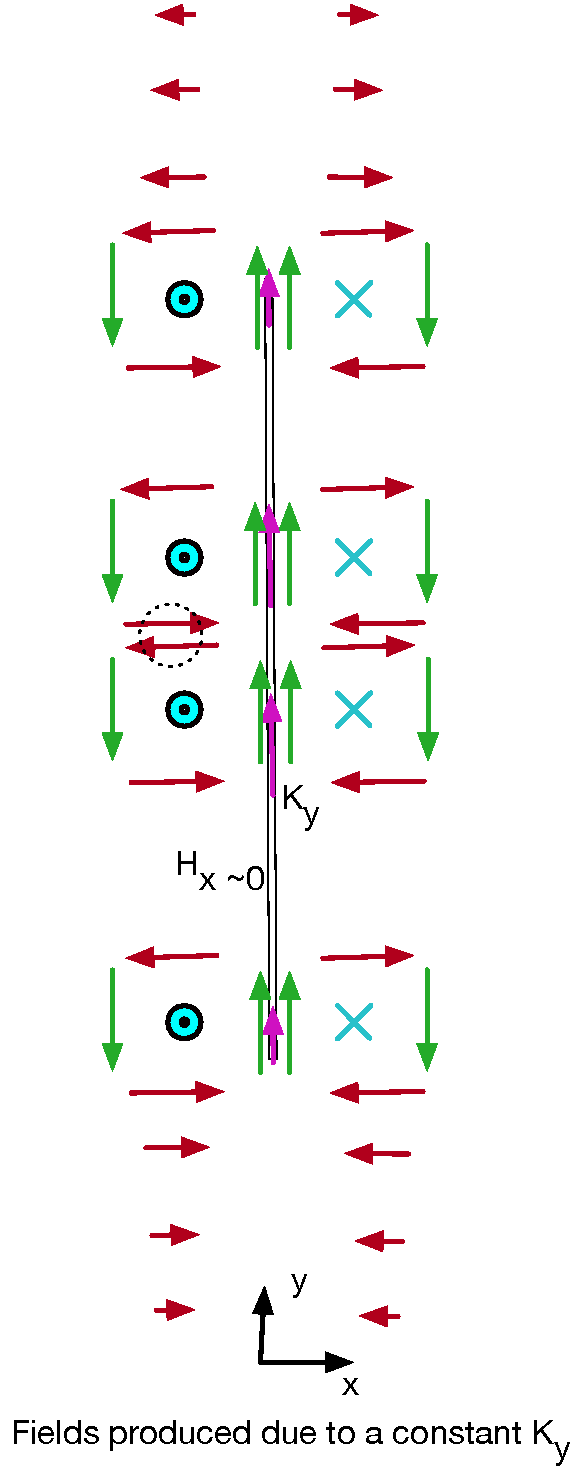
\includegraphics[width=0.24\columnwidth]{figures/OnlyKs}
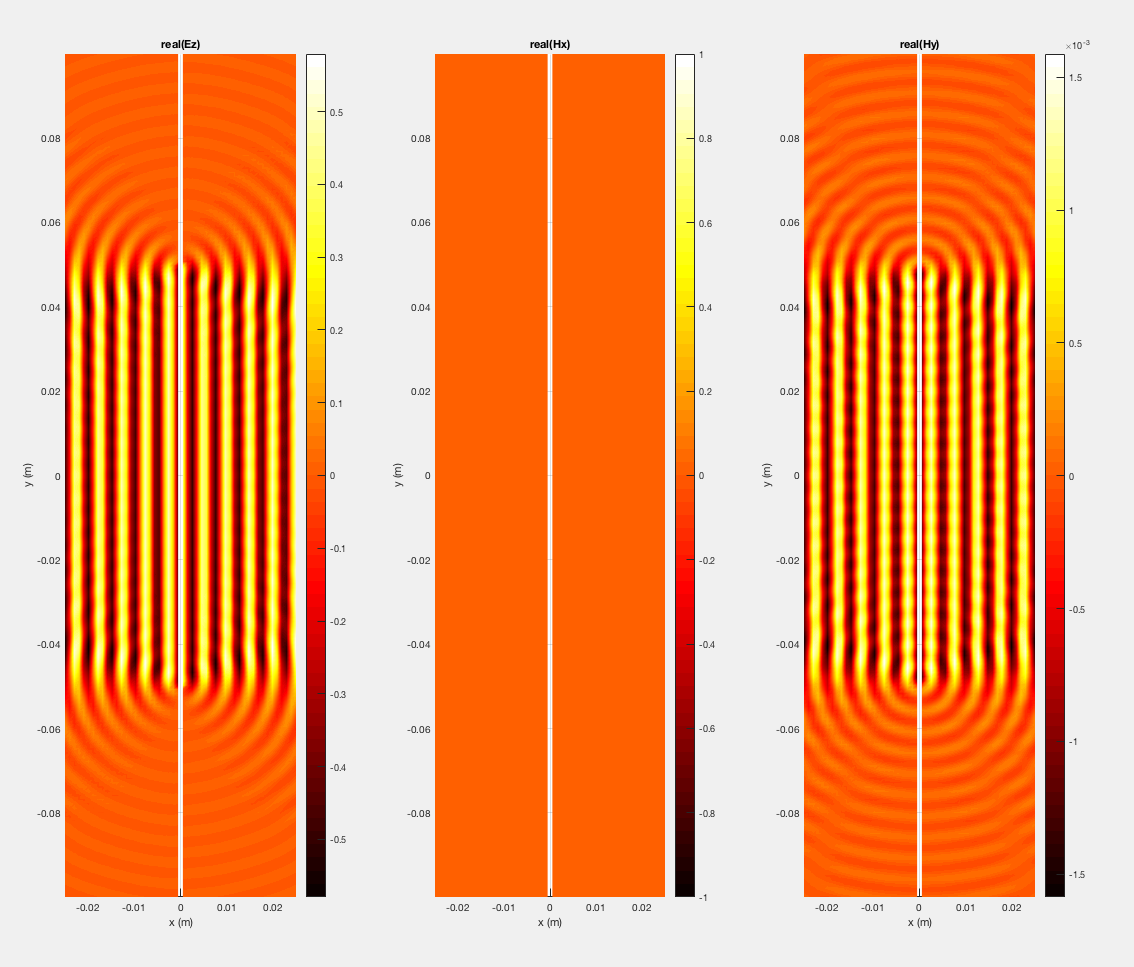
\includegraphics[width=0.74\columnwidth]{figures/OnlyKsZeroDerv.png}
\end{center}
\end{minipage}
\begin{minipage}{0.45\textwidth}
Near middle of segment we have plane-wave ($E_x, H_y$) like fields. 
\begin{enumerate}
    \item Isolated harmonic $K_y$ creates an $E_z$ field.
    \item Harmonic (time varying) $E_z$ generates $H_x$ and $H_y$ fields
    \item Near the surface the $H_x$ field is mainly ``canceled'' due to anti-symmetrical contributions from complimentary elements above and below the point. For an infinite surface this cancellation would be complete.
    \item Produces plane wave like propagation in both directions away from the surface in the center. And they are {\bf symmetric}.
    \item $H_x$ is produced by the finite length of the surface.
    \begin{enumerate}
        \item $H_x$ is anti-symmetric along the x axis (left/right).
        \item $H_x$ is anti-symmetric along y axis (top/bottom)
        \item {\bf Plot is not correct! $H_x$ is zero!}
    \end{enumerate}
\end{enumerate}
\end{minipage}

\begin{minipage}{0.45\textwidth}
\begin{align*}
    E^s(\rho) &= - (\mathcal{R}K_s)(\rho)\\
    H^s(\rho) &= -i\omega\epsilon(\mathcal{L}K_s)(\rho)\\ \\
    (\mathcal{R}K)(\rho) &= \nabla \times \int_{\ell}G(\rho,\rho')K(\rho') \,d\rho'
         = \int_{\ell} - K \times \nabla' G(\rho,\rho') \,d\rho'\\
    & K \times \nabla' G = 
    \begin{array}{|ccc|}
    \hat i & \hat j & \hat k\\
    0 & K_y & 0 \\
    \frac{\partial G}{\partial x'} & \frac{\partial G}{\partial y'} & \frac{\partial G}{\partial z'} \\
    \end{array}
       =  K_y \frac{\partial G}{\partial z'} \hat i - K_y \frac{\partial G}{\partial x'} \hat k\\
    & \rightarrow (\mathcal{R}J)(\rho) = \left[ \begin{array}{c} E_x \\ E_y \\ E_z \end{array} \right]  = 
      \left[ \begin{array}{c}  K_y \frac{\partial G}{\partial z'}\\ 0 \\-K_y \frac{\partial G}{\partial x'}  \end{array} \right] = 
      \left[ \begin{array}{c} 0\\ 0 \\-K_y \frac{\partial G}{\partial x'}  \end{array} \right]\\ \\
    (\mathcal{L}K)(\rho) &= \int_{\ell}G(\rho,\rho')[1+\frac{1}{k^2}\nabla'\nabla'\cdotp]K(\rho') \,d\rho' = \mathcal{L}_1 K + \mathcal{L}_2 K\\
    {L}_1 K &= \int_{\ell}G(\rho,\rho') K(\rho') \,d\rho' \rightarrow 
    \left[ \begin{array}{c} H_x \\ H_y \\ H_z \end{array} \right]_1 = \left[ \begin{array}{c} 0 \\ G_v K_y \\ 0 \end{array} \right]\\
    \mathcal{L}_2 K &= \int_{\ell}G(\rho,\rho')\frac{1}{k^2}\nabla'\nabla'\cdotp K(\rho') \,d\rho'\\
    \nabla'\nabla'\cdotp K &= \nabla' (\frac{\partial K_x}{\partial x} + \frac{\partial K_y}{\partial y} + \frac{\partial K_z}{\partial z}) = \nabla' \frac{\partial K_y}{\partial y} \\
    &= \frac{\partial^2 K_y}{\partial xy} \hat i + 
    \frac{\partial^2 K_y}{\partial y^2} \hat j + \frac{\partial^2 K_y}{\partial zy} \hat k =  
    \frac{\partial^2 K_y}{\partial xy} \hat i + \frac{\partial^2 K_y}{\partial y^2} \hat j \\
    &\rightarrow 
    \left[ \begin{array}{c} H_x \\ H_y \\ H_z \end{array} \right]_2 = 
    \left[ \begin{array}{c} G_v\frac{\partial^2 K_y}{\partial xy} \\ G_v\frac{\partial^2 K_y}{\partial y^2} \\ 0 \end{array} \right]\\
\end{align*}
\end{minipage}
\begin{minipage}{0.45\textwidth}
\begin{enumerate}
    \item $E_z$ is generated by the $\mathcal{R}K$ operation and involves $\partial G/\partial x$. 
    \item $E_z$ is therefore anti-symmetrical in $x$ and symmetric in $y$ as is $\partial G/\partial x$.
    \item $H$ is generated by the $\mathcal{L}K$ operation and involves two potential terms $\mathcal{L}_1K$ and $\mathcal{L}_2K$. 
    \item $\mathcal{L}_1K$ simply generates $H_y$ from G and is symmetric in $x$ and $y$.
    \item $\mathcal{L}_2K$ can generate both  $H_y$ and $H_x$ from derivatives of $K_y$.
\end{enumerate}
\end{minipage}

\newpage
Adding the two together (Both $J$ and $K$ present),
\begin{center}
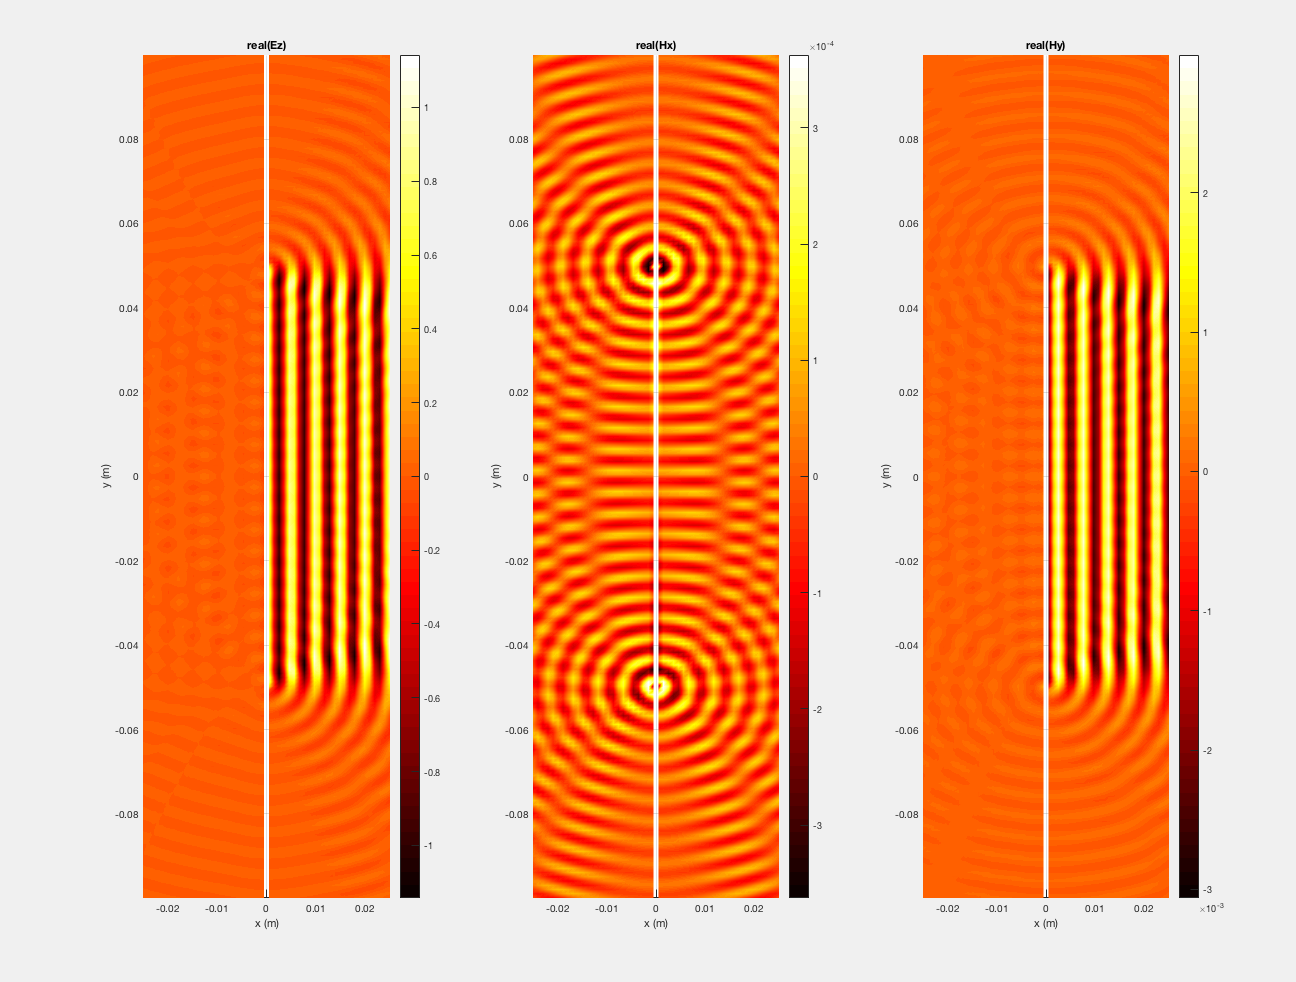
\includegraphics[width=0.25\columnwidth]{figures/Both}
\end{center}


\noindent Need to look at the generation of $H_x$ from $K_y$. $H$ fields are generated from this equation,
\begin{align*}
    H^s(\rho) &= -i\omega\epsilon(\mathcal{L}K_s)(\rho) + (\mathcal{R}J_s)(\rho)
\end{align*}
as $J = 0$ we need to look at:

\begin{align*}
    (\mathcal{L}K)(\rho) &= \int_{\ell}G(\rho,\rho')[1+\frac{1}{k^2}\nabla'\nabla'\cdotp]K(\rho') \,d\rho'\\
    (\mathcal{L}K)(\rho) &= \int_{\ell}G(\rho,\rho') K(\rho') \,d\rho' + \frac{1}{k^2} \int_{\ell} G(\rho,\rho') \nabla'\nabla'\cdotp K(\rho') \,d\rho'
\end{align*}
The first term represents the generation of the self-same component i.e. $K_x \rightarrow H_x$, $K_y \rightarrow H_y$ and $K_z \rightarrow H_z$ and this does not what do what we want.

The second term represents the gradient of a divergence of $K$ i.e. $\nabla'\nabla'\cdotp K$ and captures the phenomena of the surface coming to an abrupt end and the ``divergence'' of $K_y$ causing a generation $H_x$. However, this term has some difficulties.

Scott used terms like this,
\begin{align*}
    (\mathcal{L}_{1_{uv}}X)(\rho_n) = \sum_{m=1}^{N} \left(\frac{1}{k^2}\left(
    \frac{\partial^2}{\partial u \partial v}X_{m}
    \right)\right)\\
        \frac{\partial^2}{\partial u \partial v}X_m = \frac{X_{m+1} - 2X_{m} + X_{m-1}}{\Delta u_m \Delta v_m}
\end{align*}
to use FD to define the derivatives. This runs into issues if either $\Delta u_m$ or $\Delta v_m$ equals zero (vertical/horizontal segments). Scott sets the derivative to zero in this case -- which produced the plots above. 

\newpage
It looks like it should be large number ?? So setting it to 2000 produces this,

\begin{center}
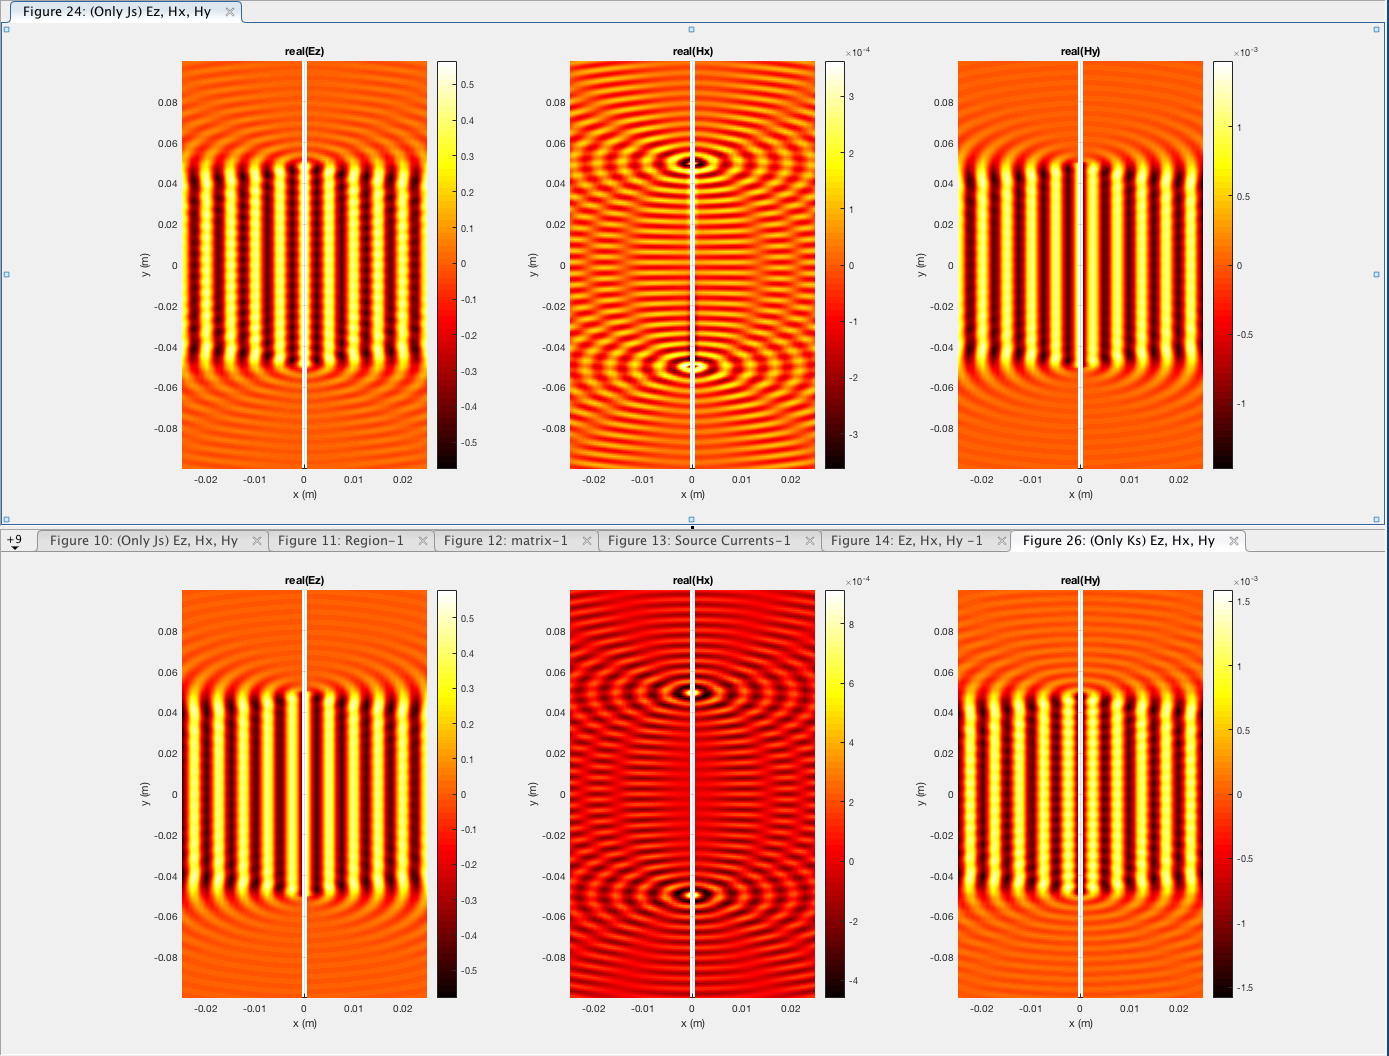
\includegraphics[width=0.55\columnwidth]{figures/Fields2000}
\end{center}


So setting it to 2000 but using the surface normal to set the sign produces this,

\begin{center}
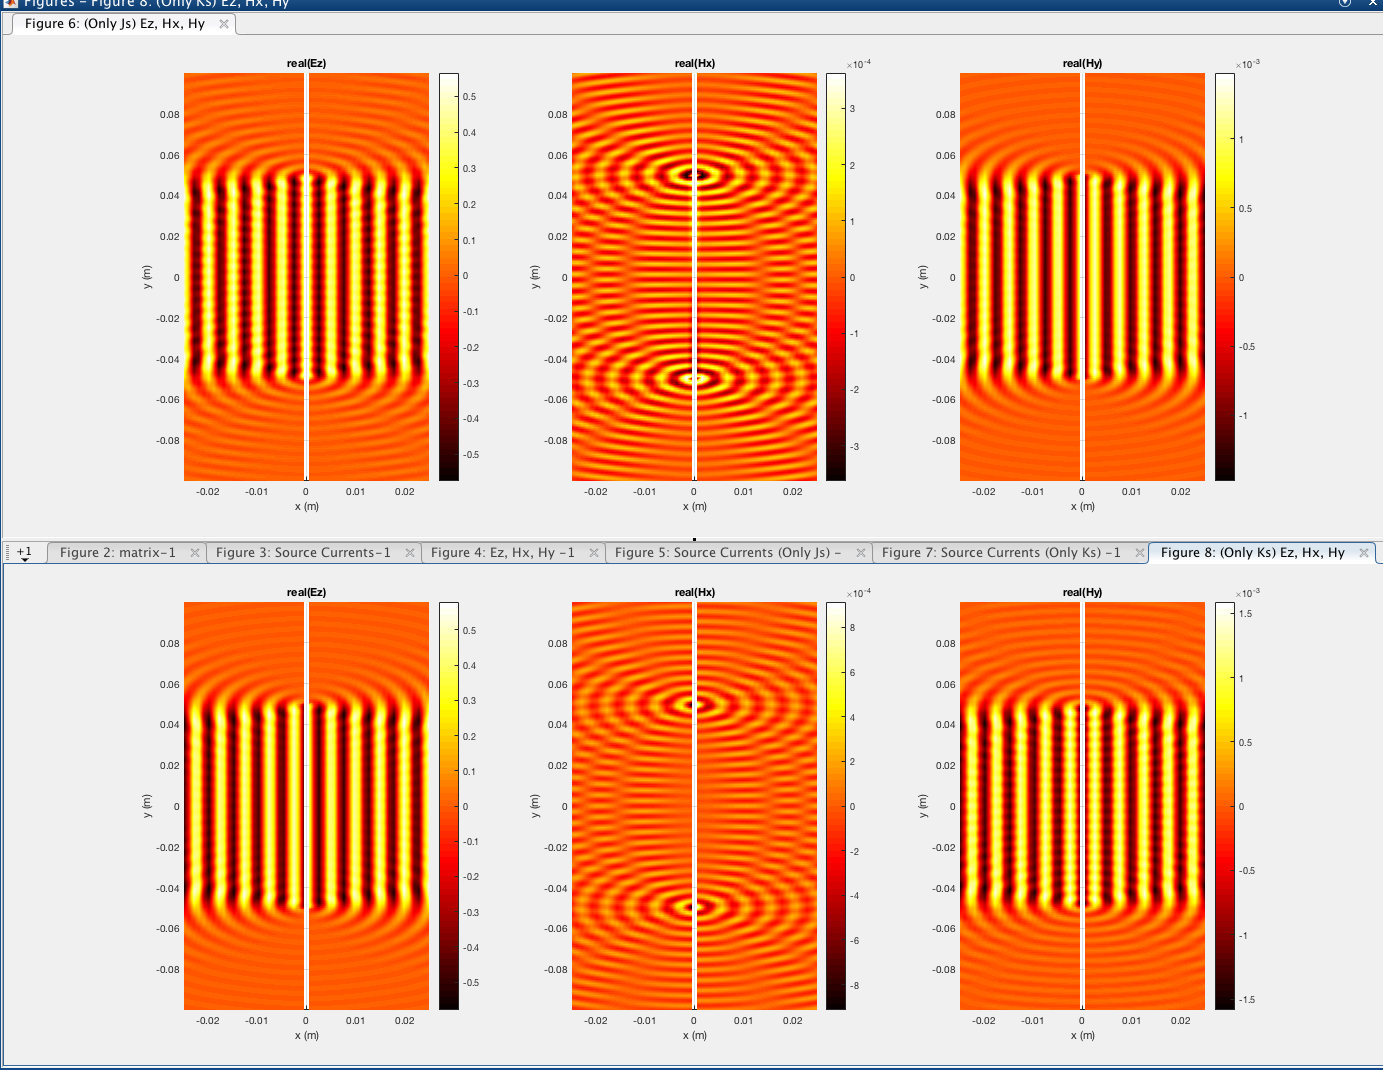
\includegraphics[width=0.55\columnwidth]{figures/Fields2000Ns}
\end{center}

\newpage
\ \\ \noindent {\bf Single segment at 45 degrees for $n = [0.707, 0.707]$ and $K = [K_x = -0.707,K_y=.707]$:}
\\ \\

\begin{minipage}{0.35\textwidth}
\begin{center}
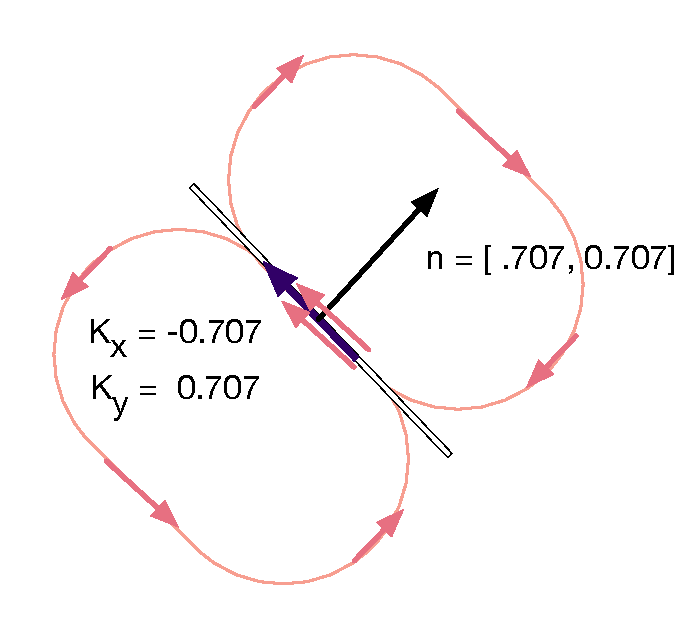
\includegraphics[width=1\columnwidth]{figures/Seg45}
\end{center}
\end{minipage}
\begin{minipage}{0.5\textwidth}
\begin{align*}
    E^s(\rho) &= - (\mathcal{R}K_s)(\rho)\\
    H^s(\rho) &= -i\omega\epsilon(\mathcal{L}K_s)(\rho)\\ \\
 \end{align*}
 \begin{align*}
    H_t &= H_x n_y - H_y n_x = 0.707 (H_x-H_y)\\
    H_n &= H_x n_x + H_y n_y = 0.707 (H_x+H_y)
 \end{align*}
 \end{minipage}
\begin{align*}
    (\mathcal{R}K)(\rho) &= \nabla \times \int_{\ell}G(\rho,\rho')K(\rho') \,d\rho'
         = \int_{\ell} - K \times \nabla' G(\rho,\rho') \,d\rho'\\
    K \times \nabla' G &= 
    \begin{array}{|ccc|}
    \hat i & \hat j & \hat k\\
    K_x & K_y & 0 \\
    \frac{\partial G}{\partial x'} & \frac{\partial G}{\partial y'} & \frac{\partial G}{\partial z'} \\
    \end{array}
       =  K_y \frac{\partial G}{\partial z'} \hat i - K_x\frac{\partial G}{\partial z'} \hat j + \left(K_x \frac{\partial G}{\partial x'} - K_y \frac{\partial G}{\partial y'}\right) \hat k\\
    & \rightarrow (\mathcal{R}J)(\rho) = \left[ \begin{array}{c} E_x \\ E_y \\ E_z \end{array} \right]  = 
      \left[ \begin{array}{c}  K_y \frac{\partial G}{\partial z'}\\ K_x \frac{\partial G}{\partial z'} \\K_x \frac{\partial G}{\partial x'} - K_y \frac{\partial G}{\partial y'}  \end{array} \right] = 
      \left[ \begin{array}{c} 0\\ 0 \\K_x \frac{\partial G}{\partial x'} - K_y \frac{\partial G}{\partial y'}   \end{array} \right]\\ \\
    (\mathcal{L}K)(\rho) &= \int_{\ell}G(\rho,\rho')[1+\frac{1}{k^2}\nabla'\nabla'\cdotp]K(\rho') \,d\rho' = \mathcal{L}_1 K + \mathcal{L}_2 K\\
    \\
    {L}_1 K &= \int_{\ell}G(\rho,\rho') K(\rho') \,d\rho' \rightarrow 
    \left[ \begin{array}{c} H_x \\ H_y \\ H_z \end{array} \right]_1 = \left[ \begin{array}{c} G_v K_x \\ G_v K_y \\ 0 \end{array} \right]\\
    \\
    \mathcal{L}_2 K &= \int_{\ell}G(\rho,\rho')\frac{1}{k^2}\nabla'\nabla'\cdotp K(\rho') \,d\rho'\\
    \nabla'\nabla'\cdotp K &= \nabla' (\frac{\partial K_x}{\partial x} + \frac{\partial K_y}{\partial y} + \frac{\partial K_z}{\partial z}) 
    = \nabla' \left( \frac{\partial K_x}{\partial x} + \frac{\partial K_y}{\partial y} \right)\\
    &= \left( \frac{\partial^2 K_x}{\partial^2 x} + \frac{\partial^2 K_y}{\partial xy}\right) \hat i + 
    \left( \frac{\partial^2 K_x}{\partial yx} + \frac{\partial^2 K_y}{\partial^2 y}\right) \hat j + 
        \left( \frac{\partial^2 K_x}{\partial zx} + \frac{\partial^2 K_y}{\partial zy}\right) \hat k\\
    &=  \left( \frac{\partial^2 K_x}{\partial^2 x} + \frac{\partial^2 K_y}{\partial xy}\right) \hat i + 
    \left( \frac{\partial^2 K_x}{\partial yx} + \frac{\partial^2 K_y}{\partial^2 y}\right) \hat j \\
    &\downarrow \\
    \left[ \begin{array}{c} H_x \\ H_y \\ H_z \end{array} \right]_2 &= 
    \left[ \begin{array}{c} G_v\left( \frac{\partial^2 K_x}{\partial^2 x} + \frac{\partial^2 K_y}{\partial xy}\right) \\ 
                            G_v\left( \frac{\partial^2 K_x}{\partial yx} + \frac{\partial^2 K_y}{\partial^2 y}\right)\\ 
                            0 \end{array} \right] = 
    G_v \left[ \begin{array}{ccc} \frac{\partial^2 }{\partial^2 x} & \frac{\partial^2 }{\partial xy}\ & 0 \\ 
                            \frac{\partial^2 }{\partial yx} & \frac{\partial^2 }{\partial^2 y} &0\\ 
                            0 & 0 &0 \end{array} \right]
        \left[ \begin{array}{c} K_x \\ K_y \\ K_z \end{array} \right]\\
\end{align*}
\begin{minipage}{0.45\textwidth}
\begin{center}
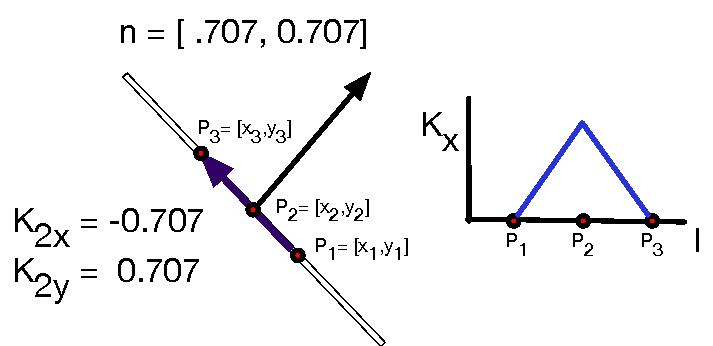
\includegraphics[width=1\columnwidth]{figures/SegDerv}
\end{center}
\end{minipage}
\begin{minipage}{0.5\textwidth}
\end{minipage}
% \end{minipage}
% \begin{minipage}{0.45\textwidth}
% \begin{enumerate}
%     \item $E_z$ is generated by the $\mathcal{R}K$ operation and involves $\partial G/\partial x$. 
%     \item $E_z$ is therefore anti-symmetrical in $x$ and symmetric in $y$ as is $\partial G/\partial x$.
%     \item $H$ is generated by the $\mathcal{L}K$ operation and involves two potential terms $\mathcal{L}_1K$ and $\mathcal{L}_2K$. 
%     \item $\mathcal{L}_1K$ simply generates $H_y$ from G and is symmetric in $x$ and $y$.
%     \item $\mathcal{L}_2K$ can generate both  $H_y$ and $H_x$ from derivatives of $K_y$.
% \end{enumerate}
% \end{minipage}

\newpage
\bibliographystyle{IEEETran}
\bibliography{Formulation2}

\end{document}